\documentclass[output=collectionpaper]{langsci/langscibook}

% \hyphenation{Lyng-ngam}

\title{The dynamics of gender complexity}

\author{Bernhard Wälchli\lastand Francesca Di Garbo\affiliation{Stockholm University}}
\abstract{In this chapter we view grammatical gender as a category type that emerges, evolves and disappears in languages as a result of diachronic processes and whose complexity grows and diminishes through time (\sectref{sec:WDG:1}--\sectref{sec:WDG:2}). Traditional approaches to grammatical gender focus on two properties that already presuppose a high degree of maturity of gender systems: noun classes and agreement. Here we conceive of gender rather as a category type with a semantic core of animacy and/or sex reflecting classes of referents, which have a propensity to turn into classes of noun lexemes. When growing and retracting, gender characteristically follows the animacy or individuation hierarchy. However, this hierarchical patterning breaks down when animacy leaks into the inanimate domain led astray by many different associative pathways, which is why lexical organization according to noun classes has to be invoked to maintain some sort of order (\sectref{sec:WDG:3}). Gender manifests itself in the form of marking on noun-associated words, often within the local domain of noun phrases. Here we put gender marking into the wider context of nominal morphology (non-lexical markers within the noun phrase), which often originate in independent use in headless noun phrases and are extended to headed noun phrases only in a subsequent development (\sectref{sec:WDG:4}). As more mature manifestations of gender get organized in the form of noun classes, they typically follow certain pathways of development that can be subsumed under the formula ``From X to Y'' (\sectref{sec:WDG:5}--\sectref{sec:WDG:6}). Agreement is fuzzy as its prototypical non-noun targets gradually develop by way of decategorialization from nouns, and controllers and targets are not always simple words, but can be complex (consist of syntactic formal groups) and controllers can be entirely contextual (\sectref{sec:WDG:7}). Gender should not be considered in isolation as it is \textendash{} more often than not \textendash{} parasitic on other grammatical category types, notably number, case, and person, with which it cumulates and which contribute to its high degree of complexity (\sectref{sec:WDG:8}). Number is particularly tightly intertwined with gender in pluralia tantum and other phenomena related to lexical plurality (\sectref{sec:WDG:9}). As gender is organized in form of systems, its diachronic evolution cannot be captured in terms of individual diachronic processes. When gender systems evolve, there is virtually always co-evolution of connected events. Hence the study of system evolution is indispensable for understanding the complexity of gender (\sectref{sec:WDG:10}). However, the evolution of gender also displays characteristic areal and genealogical patterns and is sensitive to external factors of language ecology (\sectref{sec:WDG:11}).
\medskip

\textbf{Keywords:}
gender, complexity, animacy, historical linguistics, agreement, number, pluralia tantum, system emergence, areal linguistics, language ecology

}%

\maketitle
\begin{document}

\section{Introduction}
\label{sec:WDG:1}

This chapter has no ambition to provide a comprehensive survey of the very rich literature that exists on grammatical gender, for which we refer to \citet{Corbett1991,Corbett2006,Corbett2014}, \citet{Aikhenvald2000,Aikhenvald2016}, \citet{Kilarski2013}, \citet{Heine1982}, and \citet{Seifart2010}, to mention just a few. Furthermore, no attempts are made here to strictly delimit gender from classifiers; rather, grammatical gender is our focus of interest. Moreover, this chapter does not relate grammatical gender to gender studies. Having stated what this chapter is NOT about, let us now proceed to explain its focus of interest.

This chapter represents a \spterm{dynamic approach} to the understanding of grammatical gender (henceforth simply called \textit{gender}). This means that we view gender as something that emerges, evolves and disappears in languages as a result of diachronic processes. \cite{Greenberg1978} has been an important source of inspiration for the kind of diachronic and dynamic approach we propose here. In addition to the diachronic perspective, we are also interested in assessing the complexity of gender. While in many languages gender is complex, which is why \cite[1]{Corbett1991} calls it ``the most puzzling of the grammatical categories'', different degrees of gender complexity are attested in different languages. There are also languages with simpler kinds of gender.

In this chapter we are interested in why gender can grow quite complex in some languages and remain rather simple or turn simple again in other languages. Thus, even as far as complexity is concerned, we adopt a dynamic approach. We view gender as a \spterm{mature phenomenon}. According to \cite[2]{Dahl2004}, a mature phenomenon is a phenomenon that presupposes a non-trivial prehistory. Since we are also interested in how gender comes into being in the first place, we cannot define the object of study too narrowly, as otherwise there is a risk that we will miss much of the non-trivial prehistory. Our approach to linguistic complexity, in general as well as in the domain of gender, is outlined in \sectref{sec:WDG:2}. In the following, we provide a roadmap for the topics discussed in the chapter and how they relate to the general purposes of this two-volume work.

At least since Hockett's (\citeyear[231]{Hockett1958}) succinct definition \textendash{} ``Genders are classes of nouns reflected in the behavior of associated words'', adopted by \citet{Corbett1991} \textendash{} it has been common to define gender in terms of \spterm{noun classes} and \spterm{agreement}. We argue here that noun classes and agreement are both mature phenomena.

The prototypical function of nouns is to express referents (\citealt[438]{Croft2005}; \citealt{Baker2003}). Hence, there are two different things that can be meant by noun classes: classes of noun lexemes and classes of referents. These are manifest in Dahl's (\citeyear[107]{Dahl2000a}) notions \spterm{lexical gender}, classes of noun lexemes, and referential gender, for which we use the name \spterm{referent-based gender} suggested by \citetvo{Nicholsthisyear}, classes of referents. Most approaches to gender take for granted that lexical gender is the primary object of interest, as, for instance, reflected in Corbett \& Fedden's (\citeyear[9]{Corbett2016}) Canonical Gender Principle: \emph{in a canonical gender system, each noun has a single gender value}. It is not a priori clear why it should be useful for a language to partition noun lexemes into classes, but it is immediately understandable why speakers may be inclined to classify real world objects into classes. If we adopt a dynamic approach to gender, it is thus a reasonable assumption that referent-based gender is primary and that lexical gender is a later development that does not really have any clear purpose, but is somehow hard to avoid once words bearing gender markers are constantly associated with nouns and constantly collocate with nouns. The relationship of gender and reference is discussed in \sectref{sec:WDG:3}.

\largerpage
Many researchers agree that gender always has a \spterm{semantic core}: \spterm{animacy} and/or \spterm{sex} (\citealt[101]{Dahl2000a}; \citealt[68]{Corbett1991}; \citealt{Luraghi2011}). However, somewhat strangely, this semantic core is usually not considered part of the definition of gender. The male-female sex distinction is clearly connected to animacy, as it is not applicable strictly semantically to inanimates. Animacy is thus crucial for the organization of gender. Animacy is a hierarchy rather than a simple dichotomy. Hierarchies are principles of organization that can considerably limit the complexity of a phenomenon. Hence, an important question for us to consider is how the \spterm{animacy hierarchy} relates to the complexity of gender. As far as reference and lexicon are concerned, it makes more sense to organize referents according to a semantic core, and notably according to the animacy hierarchy, than noun lexemes. In languages where nouns carry grammatical markers, the \spterm{declension classes} that structure grammatical allomorphs need not adhere to any semantic principle. This can be taken as evidence that classes of referents are crucial for the understanding of gender. The hierarchical patterning of gender is also discussed in \sectref{sec:WDG:3}.

Like other grammatical category types, gender is expressed by grammatical markers, viz.\ \spterm{gender markers}. Unlike declension classes, these are not directly realized on nouns that condition the choice of class (\citealtvo{Gueldemannthisyear}, use the term ``deriflection''), but on \spterm{noun-associated forms} (adnominal modifiers, verbal argument indexes, or anaphoric pronouns, to mention just the most important ones). Many noun-associated forms are parts of the NP, so gender marking has to do with the wider question of what kind of non-lexical marking exists within noun phrases and how this marking emerges. There are languages that get along perfectly well without any \spterm{nominal morphology} (nonlexical markers within the noun phrase). Nominal morphology is obviously a mature phenomenon. However, unlike its sub-phenomenon gender within noun phrases, nominal morphology need not necessarily distinguish classes. It can be the same marker all over, as in the \ili{English} prop-word \textit{one} for independent adjectives (adjectives without overt nominal head), as in \textit{the big one}. \cite{Lehmann1982}, \cite{Moravcsik1994}, and others have emphasized the importance of independent noun-associated elements (such as free relative clauses, pronominal demonstratives and numerals) for the development of markers on attributive modifiers. From a developmental perspective on gender, it is important to put gender into the broader context of how nominal morphology emerges and spreads across various kinds of elements in the noun phrase. This is what we discuss in \sectref{sec:WDG:4}.

Conceiving of \spterm{noun classes} in a dynamic perspective means to view them as phenomena undergoing change, which can be expressed by the formula ``\spterm{From X to Y}''. As already mentioned above, noun classes typically change from referent-based to predominantly lexical, and sometimes back to referent-based gender again (as in \ili{English}). Several types of changes in noun classes have in common that there is an increase of complexity, notably the development of several types of gender assignment, the development from semantic to opaque assignment (gender assignment characterized by numerous exceptions), and the generalization of noun classes to all nouns. The dynamics of gender assignment and its evolution are what we focus on in \sectref{sec:WDG:5} and \sectref{sec:WDG:6}.

The word \textit{complex} is ambiguous. Most of the time we are talking about complexity in this chapter we mean by it (i) non-trivial in structure, so that an exhaustive description cannot be short. But ``complex'' can also mean (ii) consisting of several elements and (iii) consisting of different, but related phenomena. In discussing agreement, meanings (ii) and (iii) will be as important as meaning (i) and it is important to discuss how they relate to each other. Since Corbett's (\citeyear{Corbett2006}) influential monograph, \spterm{agreement} has often been conceived of as a morphosyntactic feature, which emphasizes the morphological realization on word-forms and the syntactic nature of the link between controller and target. Given that there is not only intra-sentential, but also inter-sentential agreement, we hold that agreement is less uniform than commonly believed. It can be both syntactic and semantic. However, controllers and targets are not just morphological units, but often consist of several words (complex controllers and complex targets), and hence syntactic rather than morphological units. Controllers can be latent and are then neither morphological nor syntactic, but entirely contextual elements. It is often claimed that agreement always expresses coreferentiality, but coreference is actually only one of several specific relationships that may hold between controller and target. While controllers are typically nouns and targets noun-associated words, there are also nominal gender targets, and it can be shown that agreement often emerges step-by-step when nouns \spterm{decategorialize} (lose their nominal properties). To put agreement into a dynamic perspective means to recognize that agreement is not a uniform phenomenon, but rather a family of similar phenomena with complex diachronic relationships among them. We therefore suggest a broad definition of agreement, since a narrow definition is not easily compatible with a dynamic approach. This is the topic of \sectref{sec:WDG:7}.

Every definition of gender faces the problem that there is not just one, but several other grammatical category types that gender interacts with. Many researchers have recognized the close relationship to \spterm{classifiers}, and it has even become common to view gender and classifiers as one set of phenomena, for which various cover terms have been proposed, such as nominal classification (\citealt{Seifart2010}) and nomifiers (\citealt{Haspelmath2018}). At least since \cite[160]{Dixon1982}, it has been common to argue that gender is characterized by a smallish number of classes (usually between two and ten, but sometimes up to twenty) and by obligatory grouping of all nouns into noun classes. A possible dynamic interpretation would be that gender is just a more advanced stage in the grammaticalization of nominal classification than classifiers (\citealt{Passer2016b}). However, there is much reason to believe that many gender categories never went through a classifier stage (\citealt[142]{Nichols1992}). While it is undeniable that some phenomena are intermediate between genders and classifiers, a major problem of the unified account is that gender does not entertain close relationships only to classifiers, but also to a range of other grammatical category types; for instance, with indexation (\citealt{Croft2003}, \citealt{Croft2013}; see \sectref{sec:WDG:7.1}) and with person name markers (markers indicating that an element is the name of a person). It has been repeatedly observed that a majority of languages with gender exhibit \spterm{cumulation} with \spterm{number}, and cumulation of gender and \spterm{case} and of gender and \spterm{person} is also very common. This trend is so far-reaching that we think it is reasonable to include ``cumulation with number, case and/or person'' into the definition of gender (notably since such cumulation is often lacking in classifiers). In fact, to the extent that it is known how gender systems evolve, cumulation with number or case often exists from the very beginning. One reason for this is that animacy is a typical conditioning factor for the choice of number and/or case (for instance, in differential object or other differential case marking). From a condition on number or case, animacy can further develop into a gender feature (a fully paradigmaticized grammatical category type expressed by systematic morphological marking) that still maintains cumulative exponence with the grammatical categories it originates from. This suggests that gender can be mature and hence complex from the very beginning and just appropriates the complexity of other mature grammatical categories it is connected with. Thus, when we say that gender is mature this does not necessarily entail that there is a non-trivial prehistory of gender, it can be a non-trivial prehistory of another grammatical category. Cumulation of gender with number, person, and case is discussed in \sectref{sec:WDG:8}.

Beyond the patterns of cumulative exponence that make gender closely interact with the encoding of number, case, and person, \spterm{pluralia tantum} nouns, that is, nouns that only exist in the plural, and other phenomena related to \spterm{lexical plurality}, whereby plural nouns form lexical classes, may also pose delimitation problems to the definition of gender as an independent grammatical category type. A common approach is to do away with this delimitation problem by saying that pluralia tantum cannot be a gender because their special behavior stems from them being lexically specified for number, which is a separate morphosyntactic category. This way of thinking derives from the assumption that gender and number are different morphosyntactic features. However, there is growing evidence that there are languages with two largely independent \spterm{concurrent gender systems} which cannot be subsumed under one gender feature (\citealt{Fedden2017}; \citealt{Corbett2017}; \citealtvo{Svaerdthisyear}; \citealtvo{Liljegrenthisyear}). If there is not just one gender feature, why then should we assume a priori that gender and number features must always be neatly distinct? There is evidence from a dynamic perspective that pluralia tantum can develop into gender classes diachronically, which is an argument for a close relationship between gender and lexical plurality (\citealt{Dryerthisyear}, \citealt{Olssonthisyear}, both in Volume~I of this work). The relationship between gender and pluralia tantum is discussed in \sectref{sec:WDG:9}.

Gender is often called a ``\spterm{system}'', but few approaches are explicit in what this label implies. A system is minimally an opposition between at least two markers, but mature gender systems are more complex than that. They are highly organized language-specific complexes with both paradigmatic and syntagmatic components that play an important role in the architecture of grammar. Although systems can exhibit considerable complexity, there is reason to believe that they are also mechanisms to keep complexity within manageable limits. For the dynamic approach it is important to view systems as phenomena that emerge and evolve. Hence, rise, expansion, reduction and loss of gender must be viewed as processes of system evolution. This is the topic of \sectref{sec:WDG:10}.

However, the structure of gender does not only have language-internal implications. Gender exhibits specific \spterm{genealogical and areal patterns}. It has repeatedly been observed that gender is quite stable diachronically, but gender seems to be more stable in a language if the contact languages also have gender systems of the same kind. A further question is whether there are any external factors in the \spterm{ecology of languages} that condition whether languages have gender and what kind of gender systems. This and related questions are addressed in \sectref{sec:WDG:11}.

Having provided a roadmap for the main topics discussed in this chapter, we are now in a position to propose a tentative definition of gender that takes the dynamic approach into account.

\begin{quote}
Gender is a grammatical category type with a semantic core of animacy and/or sex reflecting classes of referents, which have a propensity to turn into classes of noun lexemes. It is overtly marked on noun-associated forms. It typically exhibits cumulative exponence with number, case, and/or person. Gender is organized in the form of systems.
\end{quote}

\noindent The building blocks of this dynamic definition of gender are discussed in the remainder of this chapter and based on the following outline. \sectref{sec:WDG:2} considers the relationship between gender and complexity. \sectref{sec:WDG:3} explores the relationship of gender with reference and animacy. \sectref{sec:WDG:4} discusses gender in the broader context of nominal morphology. \sectref{sec:WDG:5} and \sectref{sec:WDG:6} deal with noun classification and gender assignment. \sectref{sec:WDG:7} reconsiders the notion of gender agreement. \sectref{sec:WDG:8} investigates the relationship between gender, number, case and person while \sectref{sec:WDG:9} focuses on pluralia tantum. \sectref{sec:WDG:10} explores the extent to which gender is subject to system evolution. \sectref{sec:WDG:11} addresses gender in its genealogical and areal context and discusses the relevance of external factors in the ecology of languages. \sectref{sec:WDG:12} summarizes the results and concludes the chapter.

Since \textit{gender} is not the only term to keep track of, we have compiled an \hyperref[WDG:appendix]{appendix} with short definitions of terms at the end of this chapter. All definitions have the perspective of gender and/or complexity and their primary purpose is to facilitate the understanding of this chapter rather than being universally applicable in linguistics.

\section{Complexity and gender}
\label{sec:WDG:2}

In \sectref{sec:WDG:2.1} we provide an overview of current approaches to the notion of linguistic complexity. \sectref{sec:WDG:2.2} then discusses the relationship between complexity and gender, as well as the existing metrics of gender complexity.

  \subsection{Understanding and measuring complexity}
\label{sec:WDG:2.1}
Over the last couple of decades, the debate on linguistic complexity has focused primarily on three overarching topics:

\begin{enumerate}[label=(\roman*)]
\item what counts as linguistic complexity,
\item what to measure when quantifying complexity,
\item and what relevance this has for understanding languages overall.
\end{enumerate}

\noindent These topics, and their relevance to the understanding of grammatical gender, are tackled in the two volumes of this work, and, more specifically, in the chapters by Audring, Nichols and Sinnemäki. \citetvo{Audringthisyear} provides a theoretical account of gender system complexity by comparing the notion of linguistic complexity with canonicity and difficulty. \citetvo{Nicholsthisyear} tests and falsifies the hypothesis that languages with gender are more complex overall. \citetv{Sinnemaekithisyear} investigates whether there is a complexity trade-off between the distribution of gender systems and that of numeral classifiers across the languages of the world. A fourth contribution, \citetv{DiGarbothisyear}, approaches gender system complexity from a diachronic perspective by investigating disappearing and/or emerging patterns of gender agreement and their complexity features.

Starting with the first topic \textendash{} what counts as linguistic complexity \textendash{} all four contributions define complexity in \spterm{absolute} terms, that is as an objective property of grammatical domains rather than as a subjective feature of language use (what is also known as \emph{relative complexity}). This issue has been extensively debated in the literature. While some influential cross-linguistic studies in the field (\citealt{Kusters2003,Kusters2008}) deal with complexity as a measure of difficulty in language learning and use, the dominant approach in the functionally-oriented literature has been that linguistic complexity is best viewed as a property of language systems, rather than as a measure of ease of acquisition and use. This is essentially because we do not yet have a full account of language processing difficulties in different domains of grammar and across different modes of language acquisition. Important contributions in establishing the roadmap for such an approach to the theoretical and empirical study of linguistic complexity are the two volumes edited by \citet{Miestamo2008b} and \citet{Sampson2009}.

The second issue that has been central in the debate on language complexity is what to measure when quantifying complexity. \citetvo{Nicholsthisyear} sees two main answers to this question: (i) \textsc{inventory} or \textsc{(compositional) complexity}, that is, the number of distinctions in a grammatical system (e.g., the number of tones, tenses, genders), and (ii) \textsc{descriptive complexity} (or Kolmogorov complexity), defined as the information required to describe a system (the longer the description, the more complex the system). While Nichols sees inventory and descriptive complexity as independent of one another and argues that descriptive complexity ``is a better measure'' that ``captures well the non-transparency relevant to learnability and prone to be shaped by sociolinguistics'', an integrated approach is proposed by \citet{Miestamo2008}, and followed by \citetvo{Audringthisyear} and \citetv{DiGarbothisyear}. Under this approach, linguistic complexity is defined in terms of overall description length, which can be measured on the basis of two principles, the Principle of Fewer Distinctions and the Principle of One-Meaning--One-Form.

The \textsc{Principle of Fewer Distinctions} is a measure of inventory complexity and states that the fewer distinctions are made within a grammatical domain the less complex the domain (the fewer the tones, tense or gender distinctions, the less complex the tone, tense or gender system overall). The \textsc{Principle of One-Meaning--One-Form} is a measure of transparency whereby the less complex grammatical phenomenon is one where there is a one-to-one correspondence between meaning and form.

Under the Principle of One-Meaning--One-Form, cumulative morphemes (simultaneously expressing more than one grammatical meaning) or multiple exponents (where one grammatical meaning is distributed over several morphemes) are more complex than morphemes that are only associated with one grammatical meaning. Working specifically on the measurability of gender system complexity, \citet{DiGarbo2014,DiGarbo2016} expands this approach by proposing a third complexity principle, the \textsc{Principle of Independence}, which targets interactions between grammatical domains and their effect on the overall complexity of individual domains. Under the Principle of Independence, a marker that cumulates the encoding of gender and number distinctions features higher gender complexity than a non-cumulative marker, because the marking of gender distinctions is dependent on the number value of nouns. In the gender complexity measure proposed by \citetvo{Audringthisyear}, the Principle of Fewer Distinctions and the Principle of One-Meaning--One-Form are referred to as Principle of Economy and Principle of Transparency, while the same label as \citet{DiGarbo2014,DiGarbo2016} is kept for the Principle of Independence.

\largerpage
The third and final issue that has been frequently addressed in the literature on linguistic complexity is the relevance that complexity measures may have to understanding languages overall. Is it at all possible to design complexity metrics that allow us to estimate whether one language is generally more complex than another? And, provided that this is the case, how can such metrics be used? \citet{McWhorter2001} proposes to measure overall grammatical complexity on the basis of a pool of features ranging from phonology to syntax. However, the features suggested by \citet{McWhorter2001} aim to capture the peculiarities of one specific language profile, the creole profile, and to demonstrate that creole languages are overall less complex than non-creoles. The question thus remains whether the ambition to measure linguistic complexity overall is a feasible, and even meaningful, enterprise even beyond the creole/non-creole dichotomy. This question is approached in work by \citet{Miestamo2008}, \citet{Nichols2009}, and \citet{Sinnemaeki2014}, who argue that measures of global linguistic complexity are both theoretically and empirically unfeasible. Even assuming that the daunting task of formulating an exhaustive inventory of complexity features that are truly representative of overall grammatical complexity could be accomplished, it is still hard to establish empirically how each of these features contributes to overall complexity in comparison to others. For instance, it would be impossible to truly establish whether the presence of grammatical gender implies higher complexity than the presence of, say, grammaticalized tone distinctions, or the other way round, both within and across languages. \citet{Miestamo2008} refers to this as the problem of comparability, and argues that one way to overcome this problem is to restrict the quantitative and qualitative typological study of linguistic complexity to individual grammatical domains, and eventually compare domain-specific data with each other in search of potential complexity trade-offs between individual grammatical domains and their functional explanations. All contributions to this two-volume work approach the complexity of gender systems in the spirit of this suggestion, and even those chapters that explicitly focus on comparisons and relationships between the complexity of gender and other domains of grammar bring support to the idea that domain-specificity is a key to understanding the distribution of linguistic complexity within and across languages.

The chapter by \citetvo{Nicholsthisyear} shows that testing whether the presence of grammatical gender makes languages more complex overall produces negative results. \citetv{Sinnemaekithisyear} demonstrates that comparing gender and classifier systems in terms of complexity distributions may be useful to unravel functional trade-offs in the domain of nominal classification, whereby the presence of grammatical gender in a language disfavors the occurrence of numeral classifiers and vice versa.


  \subsection{Gender complexity metrics and the principles behind them}
  \label{sec:WDG:2.2}

Gender complexity metrics have been proposed by \cite{Audring2014,Audring2017} and \cite{DiGarbo2014,DiGarbo2016}. In their approaches, gender is considered to be a grammatical domain of its own, and its complexity is assessed on the basis of the three principles introduced in \sectref{sec:WDG:2.1}: (i) Economy, or the Principle of Fewer Distinctions, (ii) Transparency, or the Principle of One-Meaning--One-Form and (iii) (the Principle of) Independence. See \citetvo{Audringthisyear} and \citetv{DiGarbothisyear} for a more detailed treatment of the three principles.

Di Garbo's (\citeyear{DiGarbo2014,DiGarbo2016}) metric is an index of six features, each ranging between zero and one, that is applied to a dataset of 84 African languages with gender. The features are Number of gender values (GV), Nature of assignment rules (AR), Number of indexing targets (IND) (all three Fewer Distinctions), Cumulative exponence of gender and number (CUM) (One-Meaning--One-Form and Independence), Manipulation of gender assignment triggered by number/countability (M1), and Manipulation of gender assignment triggered by size (M2) (both Independence). The first three features of the metric are based on the proposal by \cite{Audring2014}. Features CUM, M1, and M2 are meant to measure the impact that interactions of gender and number, and gender and evaluative morphology, have on the overall complexity of gender. The features by \cite{DiGarbo2014,DiGarbo2016} are designed such that a simpler gender system can always take the value zero (only two genders, only semantic assignment, only one indexing target, non-cumulative exponence and no manipulation of gender). However, all languages in Di Garbo's sample have higher total values than 0.0, and many have 1.0, which can be interpreted such that gender tends to be complex at least in African languages. The metric has been applied by \citetvo{Liljegrenthisyear} to the languages of the Greater Hindu Kush area. He identifies two languages with value 0.0, \ili{Khowar} and \ili{Kalasha} (together making up the \ili{Chitral} subgroup), both of which have developed animacy-based gender distinctions quite recently. All other gender languages in Liljegren's sample have Medium or High gender complexity.

Based on the same three principles, \cite{Audring2017} develops a metric consisting of 23 features, which all can take the values \emph{simple} and \emph{complex}. The metric is illustrated only for one language, \ili{German} (\ili{Indo-European}, \ili{Germanic}), whose gender system turns out to score less than expected (only 9 of 23 features complex). This is most likely due to the fact that many simple gender features have been overlooked in the literature, while the metrics proposed by Audring allows to capture them. This metric is further elaborared upon by \citetvo{Audringthisyear} in the context of a broader discussion of the relationships between complexity, canonicity, and difficulty.

\section{Referent-based gender and the limited hierarchical patterning of gender}
\label{sec:WDG:3}

  \subsection{Introduction}
\label{sec:WDG:3.1}
In this section we are going to argue that \spterm{referent-based gender} (classes of referents) is more basic from a developmental perspective than \spterm{lexical gender} (classes of noun lexemes). Referents are typically classified in terms of animacy, and animacy is organized in form of a hierarchy. \citetvo{Nicholsthisyear} suggests that hierarchical patterning is a decomplexifying mechanism. The question thus arises as to why hierarchical patterning in gender does not limit complexity. In this section we will argue that hierarchical patterning in gender is rooted in referent-based gender and that gender typically originates as referent-based gender in the top segment of the animacy or individuation hierarchy (\sectref{sec:WDG:3.2}). However, as referent-based gender travels down the animacy hierarchy, there are two things that happen that render it less transparent. First, some or several animal gender values (animate, or, masculine and/or feminine) are expanded to inanimate objects by means of various factors often of a metonymic or metaphoric character, such as agentivity, discourse salience, uniqueness, power, purview, and possession (discussed in \sectref{sec:WDG:3.3} and \sectref{sec:WDG:3.4}). These cannot be neatly arranged on a single scale and hence hierarchical patterning fails to apply to them. Second, if gender has travelled down the animacy hierarchy, it gets increasingly more associated with nouns and is aligned with the conceptual structure of nouns, which means that it turns into lexical gender (\sectref{sec:WDG:3.5}). Noun lexemes, however, are not subject to hierarchical patterning in the same way as referents, and hence there is no hierarchical mechanism that can efficiently limit the complexity of lexical gender, even though the semantic core originating in referent-based gender is maintained. In order to prevent complete disorder, gender must thus resort to lexical patterning, instead of hierarchical patterning, and lexical patterning has a much higher degree of freedom than hierarchical patterning, which entails that complexity is less effectively limited in lexical gender. However, when lexical gender develops, referential-based gender does not disappear, but interacts with it, and lexical and referential-based gender are sometimes so similar that they are difficult to distinguish (\sectref{sec:WDG:3.6}). Both lexical and referent-based gender allow for reconceptualization of referents, which is why gender is not suitable for reference tracking (\sectref{sec:WDG:3.7}).


  \subsection{The animacy/individuation hierarchy}
\label{sec:WDG:3.2}

\cite{Dahl2000a} follows \cite{Aksenov1984} and \cite{Corbett1991} in claiming that all gender systems have a semantic core. He uses the animacy hierarchy in (\ref{ex:WDG:1})

\ea\label{ex:WDG:1}
Animacy hierarchy\\
human > higher animals > lower animals > inanimate\\
\z

\noindent to further specify that core. Above some cutoff point on the animacy hierarchy, gender is semantically assigned; below the cutoff point, gender is non-semantic (formal or arbitrary). If the animate pole is further subdivided, the major criterion is sex. From the point of view of complexity, this means that gender tends to be simple on the animate pole of the hierarchy and complex on the inanimate pole of the hierarchy, even though often the same gender values are used both above and below the cutoff point: ``inanimate nouns are quite often assigned to genders whose semantically determined core consists of animates'' (\citealt[102--103]{Dahl2000a}) and ``gender distinctions often cut through the animal kingdom'' (\citealt[100]{Dahl2000a}). A neat example is \ili{Walman} (Nuclear Torricelli, West \ili{Palai}; see \citealtvo{Dryerthisyear}), where nouns denoting humans and some larger animals are either masculine or feminine, depending on the sex of the referent, whereas nouns denoting most animals, especially non-mammals, appear to have relatively arbitrary gender, but are assigned to the same two genders masculine and feminine.

Various forms of the animacy hierarchy can be found in the literature. \cite[130]{Croft2003} uses the so-called extended animacy hierarchy (\ref{ex:WDG:2}), which, according to him, combines three distinct, but related hierarchies: person, referentiality, and animacy (\ref{ex:WDG:3}). Here and elsewhere we replace ``proper names'' by \emph{person names}, since names of animals, things, and places are usually disregarded in discussions of animacy.

\protectedex{%
\ea\label{ex:WDG:2}
Extended animacy hierarchy (\citealt[130]{Croft2003}, following \citealt[85]{Dixon1979} and \citealt{Silverstein1976}):\\
first/second person pronouns > third person pronoun > person names > human common nouns > nonhuman animate common nouns > inanimate common nouns\\
\z
}%

\protectedex{%
\ea\label{ex:WDG:3}
Component hierarchies of the extended animacy hierarchy\\
\begin{tabular}{ll}
Person:	& first, second > third (proximate > obviative)\\
Referentiality: &	pronoun > person name > common noun\\
Animacy:	& human > higher animals > lower animals > inanimate\\
\end{tabular}
\z
}%

\sloppy
As pointed out by \cite[166]{Croft2003}, different hierarchies often interact. He illustrates this with examples from\il{Panjabi, Eastern} Eastern Panjabi%
\footnote{%
Here and elsewhere in this chapter, we use mostly the language names in Glottolog in \cite{Hammarstroem2018}. Thus, here ``\ili{Punjabi}'' is replaced by ``Eastern Panjabi''.\il{Panjabi, Eastern} If Glottolog names are not used, these are given in brackets.
} %
(\ili{Indo-European}, \ili{Indo-Aryan}) for differential object marking, which combines the factors animacy and referentiality. Eastern Panjabi\il{Panjabi, Eastern} objects are overtly coded with \textit{(-)nũ} unless the object is both inanimate and non-definite (specific or non-specific). This suggests that the component hierarchy ``Referentiality'' actually falls into two \rephrase{}{different } sub-hierarchies:
Part-of-speech
(pronoun > person name > common noun) 
and Definiteness
(unique > definite > specific/referential > non-specific/non-referential).


\cite{Siemund2008} surveys pronominal gender in varieties of \ili{English} and other languages. He comes to the conclusion that pronominal gender in \ili{English} crucially depends on the degree of individuation of the entries referred to. He adduces Sasse's Individuation Hierarchy (\ref{fig:WDG:1}) to account for this, a further variant of the animacy hierarchy.

\begin{figure}[htb]
\begin{tabular}{|l|l|l|l|l|l|}
\hline person &	humans &	animals &	inanimate  &	abstracts	& mass nouns \\
names & & & tangible objects & & \\
\hline \multicolumn{2}{|c|}{humans} &	\multicolumn{4}{c|}{non-humans} \\
\hline \multicolumn{3}{|c|}{animates} &	\multicolumn{3}{c|}{inanimates} \\
\hline \multicolumn{4}{|c|}{count nouns} &	\multicolumn{2}{c|}{mass nouns} \\
\hline
\end{tabular}
\caption{Individuation hierarchy according to \cite[659]{Sasse1993}, as adapted by \citet[90]{Karatsareas2014}}
\label{fig:WDG:1}
\end{figure}

\largerpage
The individuation hierarchy is more elaborate than Croft's extended animacy hierarchy in that it contains two further sub-hierarchies: countability (count noun > mass noun) and concreteness (concrete/tangible > abstract).

Individuation is relevant in varieties of \ili{English} in various ways. Diachronically, \cite[527]{Siemund2011} show that ``gender change appears to have started with nouns ranking low in terms of individuation'' in \ili{English} in the transformation of a \ili{German}-like complex gender system to a pronominal gender system. In West Somerset \ili{English} there is a mass/count distinction (\textit{the bread} \textendash{} \textit{it}, \textit{the loaf} \textendash{} \textit{he}). For further examples from other languages, see \cite[175--217]{Siemund2008}.

  \subsection{The animacy hierarchy does not structure the connections between inanimate referents and animacy}
\label{sec:WDG:3.3}

The extended animacy hierarchy does not provide any guidelines for the domain of inanimates and the individuation hierarchy offers only three very general groupings: tangible objects, abstracts and mass nouns. However, there are various semantic connections that can link inanimate referents with animates, notably the following: agentivity, salience, purview, uniqueness, power, and possession. Possession will be addressed in \sectref{sec:WDG:3.4}, the others in this section. In these semantic domains, there are often metaphorical or metonymic connections between inanimate referents and animacy. These cannot easily be arranged on a single scale of animacy and individuation. But they all provide pathways for expansion from animate genders to the inanimate domain.

\begin{enumerate}[label=(\roman*)]
\item \textit{Agentivity}. Agents are usually conceived of as animate. Inanimate referents can leak into animate genders when they are construed as agents. In \ili{Zande} (\ili{Atlantic-Congo}, \ili{Ubangi}), nouns referring to inanimate things usually control inanimate gender, but can take animate gender when animacy is imputed on them, as in (\ref{ex:WDG:4}):

\ea\label{ex:WDG:4}
\ili{Zande} (\ili{Atlantic-Congo}, \ili{Ubangi}; \citealt[32]{Gore1926})\\
\gll Ime	ki	sa	ti-\textbf{ru}	(/ti-e)	ni	kure\\
 water	and.then	turn	\textsc{refl-\textbf{anim}}	(/\textsc{refl-inan})	with	blood.\\
\glt `And the water turned itself into blood.'\\
\z

In various languages with gender, nouns for natural phenomena are treated as animates. In his description of gender in \ili{Walman}, \citetvo{Dryerthisyear} mentions that the quasi-animate natural phenomena \textit{onyul} `earthquake', \textit{knum} `whirlpool, riptide', \textit{snar} `moon', and \textit{nganu} `sun' are masculine (unlike all other inanimates, which are feminine). \textit{Nganu} does not only mean `sun', but also `day', and is masculine in both meanings, hereby demonstrating that the gender of this noun, even though motivated by animacy and probably originating from referent-based gender, has become lexical gender.

Agentivity can come in different forms. It can be more syntactic, as in (\ref{ex:WDG:4}) where an inanimate referent is construed as an actor, or it can be more derivational, when an inanimate referent is construed as an agentive noun. Mopán Maya\il{Maya, Mopán} has masculine and feminine person name markers extended to common nouns, and one of their major functions is to form analytic agentive nouns: \textit{ix p\textquotesingle{}o\textquotesingle{}} [\textsc{gm.f} wash] `washerwoman' (``Ms wash''), \textit{aj jook\textquotesingle{}} [\textsc{gm.m} fish] `fisherman' (``Mr fish'') (\citealt[140]{Contini-Morava2018}). Gender markers can be used to suggest unexpected agentivity of inanimate objects as in (\ref{ex:WDG:5}).

\ea\label{ex:WDG:5}
Mopán Maya\il{Maya, Mopán} (\ili{Mayan}, Yucatecan; \citealt[141]{Contini-Morava2018})\\
\gll Ox-tuul-oo\textquotesingle{}	\textbf{aj}	kuch-b\textquotesingle{}äk\textquotesingle{} a	xoolte\textquotesingle{}	leek-oo\textquotesingle{}	a	b\textquotesingle{}e\textquotesingle{}\\
three-\textsc{num.clf.anim-3undergoer.pl}	\textbf{\textsc{gm.m}}	carry-meat \textsc{art}	walking\_stick	\textsc{3.emph-3undergoer.pl}	\textsc{art}	\textsc{dem.4}\\
\glt `Those aforementioned walking sticks became three (living) meat-carriermen.'\\
\z

\item \textit{Salience}. \cite{Pawley2004} shows that ``animated pronouns'' are a prominent feature in Tasmanian Vernacular \ili{English}. That there is some degree of animation can also be seen from examples where other animate words besides pronouns, such as \textit{fella}, are used, as in (\ref{ex:WDG:6}). ``The entity must be referential (specific or definite). Other factors include its importance in the discourse (as a main topic, background element, etc.), its sequential position in the discourse, and its inherent salience'' (\citealt[114]{Pawley2004}). For portable goods other than vehicles, \textit{he} expresses an attitude of detachment and \textit{she} (emotional) attachment. Plants, animals, and male genitals are \textit{he}, everything else is \textit{she}.

\ea\label{ex:WDG:6}
Tasmanian Vernacular \ili{English} (\citealt[126]{Pawley2004}): attitude of detachment\\
{[}Salesman is showing carpets to two customers{]} \textit{\textbf{That fella} he's a poly, \textbf{he}'s two fifty.}\\
\z

The classical study on animated pronouns in \ili{English} is \cite{Mathiot1978}, who observed similar patterns in spoken \ili{English} in two parts of the USA, Los Angeles County and Buffalo NY. However, for portable goods there is a polarity effect: men use predominantly \textit{she} and women \textit{he} (\citealt[134]{Pawley2004}).

\item \textit{Purview}. The notion of purview has been introduced by \cite{Gerdts2013} for \ili{Halkomelem} (Salishan, Central \ili{Salish}). \ili{Halkomelem} has a sex-based semantic gender system marked on determiners and demonstratives, where female singular humans take feminine gender and all other nouns masculine gender. However, feminine optionally appears on hundreds of inanimate nouns when they are in the feminine \spterm{purview} (\citealt{Gerdts2013}). This includes objects that belong to or relate to a female, are perceived as being feminine in size, shape, or function, or are spoken about by a female.

In Comaltepec Chinantec\il{Chinantec, Comaltepec} (\ili{Otomanguean}, Chinantecan), gender ``can be rhetorically upgraded to express a closer association than the normal gender assignment would indicate'' (\citealt[57]{Anderson1989a}). In (\ref{ex:WDG:7}), the word for `paper', which is usually inanimate, is animate in order to mark a more intimate status as a product ``of someone's personal labor and attention'' (\citealt[57]{Anderson1989a}).

\ea\label{ex:WDG:7}
Comaltepec Chinantec\il{Chinantec, Comaltepec} (\ili{Otomanguean}, Chinantecan; \citealt[57]{Anderson1989a})\\
\gll mï\textsuperscript{LM}-r	\textbf{hmi\textsuperscript{L}giú:n\textsuperscript{L}}-b	hiu\textsuperscript{LH}	ma\textsuperscript{H}hí\textsuperscript{L}\\
	request.3\textsc{pl}-3	\textbf{many.\textsc{anim}}-\textsc{affirmation}	\textsc{dim}	paper\\
\glt	`S/he asks for many papers.'\\
\z

\item \textit{Uniqueness}. In the \ili{Irish}-Canadian author Emma Donoghue's (\citeyear{Donoghue2010}) novel \textit{Room}, a mother and son are captured in a backyard shed that the boy never leaves until they manage to escape when the boy is five. In the boy's language things in Room with unique reference are \textit{he} and \textit{she}. In Room \ili{English}, feminine and masculine gender are inseparably tied to uniqueness and referentiality. In Room, \textit{Blanket} is feminine: \textit{we put Blanket over [TV] and just listen through the gray of \textbf{her}} (p.~11). However, things outside Room are all different and not unique: \textit{\textbf{it}'s not fleecy gray like Blanket, \textbf{it}'s rougher} (p.~166), \textit{Officer Oh tries to put the blanket over my head, I push \textbf{it} off} (p.~177). It may be argued that this example is artificial, but it is still a doculect of \ili{English}, and the example shows that a particular use of referent-based gender may be contextual and need not necessarily apply to a whole language as a system.

In narrative discourse, inanimates are often personified as unique referents. One of the arguments adduced by \cite[232]{Leeding1989} that gender assignment in \ili{Anindilyakwa} (\ili{Gunwinyguan}) is semantically motivated is that masculine and feminine words often are connected in traditional Dreamtime stories as dramatis personae, e.g.\ \textit{yi-ningwimwapwalhpwa akwa thi-wirrawilya} `\textsc{m}-Bat and \textsc{f}-Rainbow'. This suggests that they at least in some of their typical uses are conceived of as unique, which may have favored the extension of masculine and feminine to inanimates.

\item \textit{Power}. \cite{Straus1982} have argued that the seemingly arbitrary distribution of animate and inanimate gender for inanimate referents in \ili{Algonquian} languages is motivated by power. Animate nouns are all in some sense ``powerful'' (\citealt[135]{Straus1982}). In \ili{Cheyenne} (\ili{Algic}, \ili{Algonquian}, \ili{Cheyenne}), some body parts (finger/toe, thumb, fingernail, claw, eyebrow, knee, kidney, and brain) are animate, but not when indicated on a drawing or discussed as abstractions, and there is a good story for each of them why exactly these are powerful (\citealt[128--130]{Straus1982}). \ili{Cheyenne} \textit{mo?eško} `finger, toe', for instance, is animate because fingers are used symbolically as weapons and as channels of power in cursing, but there is also an inanimate noun \textit{mo?eško} `ring'. Power has cultural implications. However, whether ascribed to language or culture, the classification of nouns is complex and on some level due to convention. ``For example, nouns labeling mechanical items introduced by Whites are largely inanimate in \ili{Ojibwa} while they are often animate in Menomini'' [\ili{Menominee}] (\citealt[133]{Straus1982}). This suggests that referent-based animate gender of inanimates, originally motivated by the factor power, has largely turned into lexical gender in \ili{Algonquian} languages.
\end{enumerate}

  \subsection{Inherited gender}
\label{sec:WDG:3.4}

A further semantic connection between animate and non-animate referents is possession, which is even more difficult to include in the animacy hierarchy. In \textsc{inherited gender}, surveyed by \cite{Evans1994} for Australian languages, the gender of a noun or NP is determined by the gender of its possessor. Inherited gender is usually referent-based rather than lexical gender, and this is stated explicitly by \cite[186]{Olsson2017} for \ili{Coastal Marind} (\ili{Anim}, Marindic). In \ili{Coastal Marind}, a few nouns, including \textit{igih} `name' in (\ref{ex:WDG:8}), inherit the gender of the referent to which they are attached.

\protectedex{%
\ea\label{ex:WDG:8}
\ili{Coastal Marind} (\ili{Anim}, Marindic; \citealt[187]{Olsson2017})\\
\gll igih	\textbf{ta/tu/ta/ti}	ka-ha-b\\
name	\textbf{what:I/what:II/what.III/what.IV}	\textsc{prs.neut-int-act[3sg.a]}\\
\glt `What is his/her/its name?' more literally: `What is the he-name, she-name, it-name?'\\
\z
}%

Note that the possessive pronoun in the \ili{English} translation is misleading. The interrogative pronoun simply takes the gender that the speaker assumes to be the class of the referent (male name for gender I, female or nouns denoting animals for class II, thing of a noun in class III or IV for class III and IV; \citealt[187--188]{Olsson2017}). For inherited gender in New Guinea, see also \cite[177]{Fedden2011}.

In \ili{Halkomelem}, inherited gender is part of the extension of feminine to inanimates by purview. In example (\ref{ex:WDG:9}), the instrument \textit{šəptən} `knife' can be feminine if possessed by a female, but must be masculine when possessed by a male:

\ea\label{ex:WDG:9}
\ili{Halkomelem} (Salishan, Central \ili{Salish}; \citealt{Gerdts2013})\\
\gll niˀ	ˀəncə	kʷθə/\textbf{łə}	šəptən-s	θey̓	q̓emiˀ?\\
\textsc{aux}	where	\textsc{det}/\textbf{\textsc{det.f}}	knife-3.\textsc{poss}	\textsc{dem.f}	girl\\
\glt `Where is that girl's knife?'\\
\z

In North America, inherited gender is also attested in \ili{Tunica} (isolate), where body parts inherit gender (\citealt[23]{Swanton1921}).

It is important to emphasize that inherited gender is not always referent-based gender. In \ili{Jarawara} (\ili{Arawan}, Madi) inalienable possession, the gender of the NP is determined by the gender of the possessor. The \ili{Arawan} languages have complex lexical gender assignment. It is thus not surprising that even inherited gender in \ili{Jarawara} is more complex than in \ili{Halkomelem}, where there is virtually no lexical gender anywhere in the language. In \ili{Jarawara}, it is the lexical gender of the possessor that is inherited, not the gender of the referent. Pronouns are feminine irrespective of referent-based gender (\citealt[489]{Dixon2000}).\footnote{%
\ili{Jarawara} is not the only language where pronouns all trigger a specific gender. In \ili{Uduk} (\ili{Koman}; \citealtvo{Killianthisyear}) pronouns are always in class 1.
} %
Hence, the NP in (\ref{ex:WDG:10}) is feminine and triggers feminine agreement on the predicate, whatever the sex of the referents. As we will see in \sectref{sec:WDG:7.3}, this is a kind of gender resolution. However, some inalienable nouns also have derivational gender suffixes, whose gender is determined in a different and rather complex way, but also by the lexical gender of the possessor. A first person inclusive possessor, as in (\ref{ex:WDG:10}), always triggers masculine derivational gender. This is an instance of a nominal target (see \sectref{sec:WDG:7.6}), where a derivational affix of a noun can be an agreement target.

\ea\label{ex:WDG:10}
\ili{Jarawara} (\ili{Arawan}, Madi; \citealt[490]{Dixon2000})\\
\gll Ee 	man-\textbf{o} 	koma-\textbf{ke}\\
1\textsc{pl.incl.inalien} 	arm-\textbf{\textsc{deriv.m}} 	be.sore-\textbf{\textsc{decl.f}}\\
\glt `Our (inclusive) arms are sore.'\\
\z

In Australian languages it is common to mix inherited gender and intrinsic lexical gender. In \ili{Mawng} (Iwaidjan Proper), some nouns for body parts, such as  \textit{ngijalk} `body', always have inherited gender, whereas \textit{ngaralk} `tongue' (class IV), \textit{murlu} `nose' (class III) and \textit{algij} `liver' (class V) can have lexical gender (\citealt{Capell1970}; \citealt[5]{Evans1994}). In \ili{Tiwi} (isolate), body part nouns take the gender of their possessor, except for genitals that take the gender of the opposite sex (\citealt[2]{Evans1994}). The opposite choice for genitals can be explained by purview. Genitals relate to the other sex. Opposite choice is also attested for the Amwi variety of \ili{War-Jaintia}\il{War-Jaintia, Amwi variety} (\ili{Austroasiatic}, \ili{Khasian}; \citealt{Weidert1975}): \textit{ʔu kdɛ} `\textsc{det.m} vagina', \textit{kə khlɛ} `\textsc{det.f} penis'. However, inverted inherited gender, i.e.\ gender opposite to that of the referent of the possessor, is generalized in \ili{Amwi} War. Body parts, tools and household items take the gender opposite to the person they are associated with. Inverted inherited gender in \ili{Amwi} War exhibits the same fluidity as non-inverted inherited gender in \ili{Halkomelem}, and this suggests that we have to deal with referent-based gender rather than with lexical gender here: \textit{ʔu khlia kə} [\textsc{det.m} head 3.\textsc{sg.f}] `her head' (personal pronouns preposed to nouns are gender markers of that noun, possessors are postposed to their heads in NPs), \textit{kə klia-w} [\textsc{det.f} head-3.\textsc{sg.m}] `his head'. Only tools and clothes only associated with one sex are not fluid, in the same way as genitals: \textit{kə cin} `jeans (only for men)'.

Inherited gender and gender by purview is a kind of associated gender. The most famous case of associated gender in the literature is \ili{Dyirbal}. \cite[16]{Corbett1991} uses the term concept association for the well-known \ili{Dyirbal} examples where `fishing line' and `fish spear' are gender I (animate) because of their association with `fish' (but see \citealt{Plaster2007} for an alternative explanation). In the light of the many examples of association by referent surveyed in this section it seems to us that the term ``concept association'' is problematic. Association in gender is mainly association with referents and not association with concepts. Of course, as in other cases where referent-based gender turns into lexical gender, association of referents can eventually turn into association of concepts.

Not only are the semantic connections discussed in \sectref{sec:WDG:3.3} and this section often metonymical or metaphorical in character, some of them also provide pathways for how cultural beliefs can make their way into language structure. This holds in particular for purview and power. If we conceive of gender as referent-based originally, it does not necessarily express cultural beliefs from its very origin. There are many languages with semantic gender assignment where there is no associated gender of the kind that is attested in \ili{Dyirbal} and \ili{Algonquian} languages. There is no reason to believe that communities speaking languages without associated gender are poorer in their cultural beliefs. It is thus possible to view the ``culturalization'' of gender as a trait of maturity. Languages with many cultural properties embedded in grammatical gender presuppose gender categories with non-trivial prehistories.

  \subsection{Lexical gender originates from referent-based gender}
\label{sec:WDG:3.5}

In \sectref{sec:WDG:3.2} and \sectref{sec:WDG:3.3} we have considered cases where referent-based animate gender leaks to inanimate referents. In this section we will now consider instances of referent-based gender marking that have further developed into lexical gender as gender has travelled down the animacy hierarchy from personal pronouns and person names to NPs headed by common nouns.


\ili{Russian} and other \ili{Slavic} languages have developed a lexical animacy distinction in addition to the three-way masculine-feminine-neuter lexical gender system inherited from \ili{Indo-European}. \ili{Slavic} animacy subgenders originate from differential object marking. Due to sound change, nominative and accusative singular came to be morphologically indistinguishable in the major masculine declension class, which is why forms of the genitive singular started being used in object function (\citealt{Meillet1897}; \citealt[206]{Huntley1980}), and the genitive form was then also used in non-object function following prepositions. In \ili{Old Russian} of the 13th and 14th centuries, genitive singular forms had generally replaced accusative forms for personal pronouns and person names (\citealt[263]{Dietze1973}). According to \cite[265]{Dietze1973}, socioeconomically subordinate and dependent persons, such as children, servants, slaves, and messengers, go with the inanimate category; \textit{mužь} `man' is animate in the meaning `husband' but inanimate as the subjects of a prince, and \textit{vinogradъ} `vineyard' is animate when used metaphorically for the world populated with people, as in (\ref{ex:WDG:11}). Hence, animacy gender on masculine singular common nouns was referent-based in \ili{Old Russian}.

\ea\label{ex:WDG:11}
\ili{Old Russian} (\ili{Indo-European}, \ili{Slavic}; \citealt[267]{Dietze1973})\\
\gll gospodi	bože...	posěti	svo\textbf{ego}	vinograd\textbf{a}\\
lord.\textsc{voc.sg}	god.\textsc{voc.sg}...	visit(\textsc{pfv}).\textsc{imp.2sg}	own.\textbf{\textsc{gen.sg.m}}	vineyard(\textbf{\textsc{m/anim}}).\textsc{gen.sg}\\
\glt `O Lord God...visit your vineyard'\\
\z

Animate forms with animals start appearing in the 16th century, and in the 17th century, animate forms for animals were generalized (\citealt[270]{Dietze1973}). (\ref{ex:WDG:12}) from Modern \ili{Russian} illustrates that animate gender has become lexical. Even though the Modern \ili{Russian} animacy distinction is clearly semantically motivated, it is entrenched in the lexicon and some modern dictionaries now indicate whether a noun is animate or inanimate. In (\ref{ex:WDG:12}) \textit{konkurent} `competitor' is animate (takes genitive singular in object function) and \textit{Uzbekistan} is inanimate (takes nominative singular in object function), although they both have the same referent.

\ea\label{ex:WDG:12}
\ili{Russian} (\ili{Indo-European}, \ili{Slavic}): lexically entrenched animacy distinction\\
\gll Kazaxstan-Ø	rassmatrivaet	Uzbekistan-\textbf{Ø}	kak	konkurent-\textbf{a}.\\
K.(\textsc{inan/m)-nom.sg}	view(\textsc{ipfv}).\textsc{prs.3sg}	U.(\textsc{inan/m})-\textbf{\textsc{nom.sg}}	how/as	competitor(\textsc{anim/m})-\textbf{\textsc{gen.sg}}\\
\glt `Kazakhstan views Uzbekistan as a competitor.'\\
\z

Gender marked on NP-markers may develop from person name markers. Person name markers have a tendency to be expanded. Varieties of \ili{Catalan} have the person name markers masculine \textit{en} (< \textit{don} < \ili{Latin} \textit{dominus}) and feminine \textit{na} (< \textit{dona} < \ili{Latin} \textit{domina}). In Balearic \ili{Catalan}, these markers can be expanded to names of animals (\textit{en Pluto} for a male dog), and to folk names of clouds and celestial bodies: \textit{en Catalí} `Venus at dawn' (\citealt[195--197]{CaroReina2018}). This is arguably not lexical gender, since common nouns are not involved, but referent-based gender having traveled down the animacy hierarchy. Person name markers are very common in \ili{Austronesian} languages, where they are sometimes extended to some older kinship terms, such as `father' and `mother', which are often unique, or titles.%
\footnote{%
It should be noted here that uniqueness does not have the same effect in gender as in definiteness, where it has also been claimed to play an important role \citep{Russell1905,Lyons1999}. Definite articles are used in the first place with concepts that are not unique out of context, but which happen to be unique in a particular situation. Person name markers, however, express uniqueness on items that are unique in any context and are extended first of all to expressions that are typically construed as unique.
} %
Like many other \ili{Austronesian} languages, \ili{Tagalog} (Central Philippine) makes a distinction between noun phrase markers for common nouns (topic \textit{ang}, non-topic \textit{nang}, oblique \textit{sa}) and for person names (topic \textit{si}, non-topic \textit{ni}, oblique \textit{kay}). Person name markers can also be used with older kinship terms (\textit{ate} `eldest sister', \textit{kuya} `eldest brother', \textit{ina/nanay} `mother', \textit{ama/tatay} `father' and some others); the difference is that this use is optional. They can be used with nouns designating occupations when expressing titles: \textit{si Abogado Cruz} `Lawyer Cruz' (\citealt[94]{Schachter1972}). In several \ili{Oceanic} languages, person name markers have been extended to some common nouns and turned into lexical gender. In \ili{Nakanai}, the person name marker is used with about 70\% of the names of species of fish, birds and insects and a majority of loanwords (\citealt[166--167]{Johnston1980}). For \ili{Teop}, see \citetvo{Svaerdthisyear} and the references given there; for \ili{Owa} and \ili{Kahua}, see \sectref{sec:WDG:6.4}; and for \ili{Austronesian} in general, see \cite{Handschuh2018}.

In the \ili{Mek} languages in New Guinea it can be observed how lexical gender can develop from a referent-based gender uniqueness vs.\ non-uniqueness distinction, where uniqueness looks very much like an extended person name marking. The more conservative \ili{Mek} languages \ili{Una} and \ili{Eipo} [=Eipomek] have a uniqueness distinction, and \ili{Nalca}, which is more progressive and closely related to \ili{Eipo}, has developed a gender system with four lexical gender classes with rather simple gender assignment principles (\citealt{Waelchli2018}).

\ili{Una} has only an opposition between \textit{bi-} unique and \textit{a-} non-unique. \textit{Bi-} is mainly used with person names and kinship terms older than ego \textendash{} thus the cutoff point on the animacy hierarchy is between older and younger kin \textendash{} but also with highly individuated non-kinship human nouns and sometimes even animals and things. Thus, in the \ili{Una} New Testament, \textit{bi-} occurs, for instance, with \textit{ner} `woman' where it means `queen', with \textit{Mi} `child, son' only when it is the `Son of God' (capitalization in orthography has a function similar to the uniqueness marker), and with \textit{Uram} `voice, word' only when it is `God's voice'. (\ref{ex:WDG:13}) illustrates its use with a person name as opposed to \textit{a-} with common nouns. Note that \ili{Una} also can mark person names with preposed third person pronouns not distinguishing gender (\textit{Er Jesus} `he Jesus') and that the two strategies can be combined, as exemplified in (\ref{ex:WDG:13}).

% \protectedex{%
\ea\label{ex:WDG:13}
\ili{Una} (Nuclear \ili{Trans-New Guinea}, \ili{Mek}; New Testament 41009020)\\
\gll Ba,	sun-ci	a	mi	\textbf{a-si}	Er	Yesus	dam	bo-ya-nmai	ura, a	mi	wek-am-we	isa	\textbf{a-ryi}	Er	Yesus	\textbf{bi-si}	asing	eib-mou	ura,	a	mi	\textbf{a-si}	tomob-oka	oublob-mou.\\
but	they-\textsc{erg}	this	child	\textbf{\textsc{n.uni-acc}}	\textsc{3sg}	Jesus	near	carry-come-\textsc{pst.3pl} after this	child	enter-previously-\textsc{pst.3sg}	ghost	\textbf{\textsc{n.uni-erg}}	\textsc{3sg}	Jesus	\textbf{\textsc{uni-acc}}	eye	see-\textsc{pst.3pl}	after	this	child	\textbf{\textsc{n.uni-acc}}	erect-\textsc{cvb}	crush-\textsc{pst.3sg}\\
\glt `And they brought this child to Jesus. And when the ghost who had entered the child saw Jesus, the spirit immediately convulsed the child...'\\
\z
% }%

\begin{figure}%
\resizebox{\textwidth}{!}{\begin{tikzpicture}[baseline,nodes={text height=.7em, text depth=.2em}]%
% Ø &	\multicolumn{2}{c}{<---SINGULAR----------- \textit{bi-}} &	\multicolumn{4}{c}{\textit{a-} ---------------------------------------------------------->}\\
% Ø	& \multicolumn{6}{c}{<---PLURAL--------a------------------------------------------------------------------------->}\\
\node at (0,0) [align=center,anchor=base west] (persp) {\strut personal\\pronouns};
    \node[right=1em of persp.base east,anchor=base west,align=center] (persn) {\strut person\\names};
        \node[align=center,right=1em of persn.base east,anchor=base west] (kinolder) {\strut kinship terms\\older than ego};
            \node[align=center,right=1em of kinolder.base east,anchor=base west] (kinyounger) {\strut kinship terms\\younger than ego};
                \node[right=1em of kinyounger.base east,anchor=base west] (humans) {\strut humans};
                    \node[right=1em of humans.base east,anchor=base west] (animates) {\strut animates};
                        \node[right=1em of animates.base east,anchor=base west] (things) {\strut things};
\draw [decoration=brace,decorate] (kinolder.south east) -- (persn.south west) node[midway,below=2.5\baselineskip,align=center] {prominent animates\\\itshape masculine nominalizations\\\itshape masculine demonstrative};
\node[above=\baselineskip  of persp.north,align=center,anchor=base] (emptyset1) {∅};
\node[above=2\baselineskip of persp.north,align=center,anchor=base] (emptyset2) {∅};
\node[above right=2\baselineskip and .25em of kinyounger.north west,anchor=base] (a) {\itshape a-};
\node[above left=2\baselineskip and .25em of kinolder.north east,anchor=base] (bi) {\itshape bi-};
    \node [above=2\baselineskip of things.north east,anchor=base] (UpperEast) {};
    \node [above=\baselineskip of things.north east,anchor=base] (LowerEast) {};
    \node[above=2\baselineskip of persn.north west,anchor=base] (UpperWest) {};
    \node[above=\baselineskip of  persn.north west,anchor=base] (LowerWest) {};
\node[right=3em of UpperWest.base east,anchor=base] (singular) {\scshape singular};
\node[right=3em of LowerWest.base east,anchor=base] (plural) {\scshape plural};
\draw [->] (a) -- (UpperEast);
\draw [->] (bi) -- (singular) -- (UpperWest);
\path (plural) edge [->] (LowerWest)
               edge [->] node[pos=.1,fill=white] {\itshape a} (LowerEast);
\end{tikzpicture}}%
\caption{Una \textit{bi-} unique and \textit{a-} non-unique and the animacy hierarchy}
\label{fig:WDG:2}
\end{figure}


The \ili{Una} gender system can thus largely be characterized by the animacy hierarchy in \figref{fig:WDG:2}. There are two anomalies (in italics in \figref{fig:WDG:2}). There is a masculine singular nominalizing suffix \textit{-nyi}, often used in indigenous names, and nominalizations suffixed by \textit{-nyi} are always unique \textit{bi-}.%
\footnote{%
We will return to \ili{Mek} nominalizations in \sectref{sec:WDG:7.3} in the discussion of complex controllers.
} %
The same marker \textit{-nyi} can also be added to the demonstrative \textit{a-}, which then together with \textit{bi-} unique can serve as a masculine grammatical anaphor (but is different from the third person pronoun which does not distinguish gender). These anomalies are the germs for a further development of the \ili{Una} unique marker \textit{bi-} towards a lexical masculine gender \textit{be-} in \ili{Nalca} (see \citealt{Waelchli2018} for the details).

In a wide range of languages from different places in the world, noun markers, whether they distinguish gender or not, are so called \spterm{pronominal articles} (\citealt[838]{Himmelmann2001}), which means that noun markers have the same form as personal pronouns (mainly third person pronouns, but occasionally also second and first person) and have developed from personal pronouns (unlike \ili{Romance}, where both articles and personal pronouns independently originate from demonstratives). For the development of pronominal articles from personal pronouns in \ili{Kxoe} (\ili{Khoe}-Kwadi, \ili{Khoe}), see \cite[231--234]{Heine1984}. Interestingly, many languages with pronominal articles with gender, such as the \ili{Khoekhoe} language \ili{Nama} (\ili{Khoe}-Kwadi, \ili{Khoe}), \ili{Khasi} (\ili{Khasian}, \ili{Austroasiatic}), \ili{Mian} and \ili{Oksapmin} (\ili{Ok}-\ili{Oksapmin}, Nuclear \ili{Trans-New Guinea}), \ili{Abau} (\ili{Sepik}), \ili{Kayabi} and \ili{Tenharim} (\ili{Tupian}, Tupi-Guarani), use pronominal articles with proper names (except in vocatives and non-referential use where a person is given a name), in contrast to articles from other origins, which are rarely used with proper names. This suggests that person names may play an important role when pronouns extend to articles, and a reasonable hypothesis is that pronominal gender can expand to nouns by travelling down the animacy hierarchy, among other things via person names. Evidence that pronominal articles travel down the animacy hierarchy comes from languages where pronominal articles are less grammaticalized and restricted to human or animate referents. In \ili{Oksapmin} (\citealt[178--184]{Loughnane2009}), pronominal articles occur with specific human referents, but usually not with things or animals, where the definite article (of demonstrative origin) is used (\ref{ex:WDG:14}).

\ea\label{ex:WDG:14}
\ili{Oksapmin} (Nuclear \ili{Trans-New Guinea}, \ili{Ok}-\ili{Oksapmin}; \citealt[180]{Loughnane2009})\\
\gll robin	\textbf{ux}=nuŋ	bəp	ulxe	ap	\textbf{jox} o=m-de-pti\\
Robyn	\textbf{3\textsc{sg.f}}=\textsc{obj}	so	3\textsc{sg.f.refl.poss}	house	\textbf{\textsc{def/dem}} leave=\textsc{prox.obj}-make-\textsc{ipfv.pl.prs}\\
\glt `After that, we left Robyn at the house.'\\
\z

The \ili{Oksapmin} definite article (a demonstrative) may co-occur with the pronominal article and the order is then noun-definite.article-pronominal.article: \textit{nap jox ux} [younger.sister \textsc{def/dem 3sg.f}] `the younger sister' (\citealt[128]{Loughnane2009}). In \ili{Oksapmin}, pronominal articles can be used with animals, when a specific animal is opposed to another one, or for mythical animals with human-like characteristics. Pronominal articles can also occur with forces of nature. There does not seem to be any lexical gender in \ili{Oksapmin}. Feminine is restricted to female human referents. \ili{Oksapmin} thus provides support for the hypothesis that, if expressing gender, pronominal articles mark referent-based gender at first, and can later turn into markers of lexical gender, if their extension to inanimate nouns is more advanced.


  \subsection{The relationship between referent-based and lexical gender}
\label{sec:WDG:3.6}

The preceding sections might have evoked the idea that referent-based and lexical gender are strictly opposed to each other, but this is actually not the case. To the extent that lexical concepts denote sets of referents that are homogeneous with respect to the referent-based properties distinguished in gender, there is no mismatch.

The best-known mismatches are so-called \spterm{hybrid nouns}, such as \ili{German} \textit{Mädchen}, which is neuter as a lexical noun (due to its diminutive suffix \textit{-chen}, which morphologically assigns neuter gender to the lexeme), but refers to female beings. In cases of conflict, lexical gender is more likely in local than in distant agreement, where semantic agreement (referent-based gender) prevails, which is Corbett's well-known Agreement Hierarchy (\ref{ex:WDG:15}).

\ea\label{ex:WDG:15}
The Agreement Hierarchy (\citealt[226]{Corbett1991})\\
attributive < predicate < relative pronoun < personal pronoun\\
\textit{ein nettes} [\textsc{n}] \textit{Mädchen} (\textsc{n}), \textit{das} [\textsc{n}] \textit{ich kenne. Sie} [\textsc{f}]...\\
`a nice girl whom I know. She...'\\
\z

We assume here that lexical gender is the special case and referent-based gender is the rule. Lexical gender need only be invoked if gender in a language cannot be captured in terms of the animacy or individuation hierarchy. If a language distinguishes marking associated with person names as opposed to common nouns, such as \ili{Tagalog}, discussed in \sectref{sec:WDG:3.5}, there is no need to invoke lexical gender.

Now, many languages with lexical gender still have choices of gender values that are reminiscent of referent-based gender. Thus, \ili{Swedish} (\ili{Indo-European}, \ili{Germanic}) makes a distinction between the mass noun \textit{öl} `beer' (neuter gender) and \textit{en öl} `one.\textsc{cm} beer' (common gender) when it is countable as a glass or a bottle of beer. This distinction is well in-line with the individuation hierarchy, but it is also lexical, since most \ili{Swedish} nouns denoting liquids do not follow the same pattern.

Plains Cree (\ili{Algic}, \ili{Algonquian}, \ili{Cree}) \textit{mistik} means `tree' when animate and `stick' when inanimate (\citealt[22]{Wolfart1973}; similarly in \ili{Cheyenne}, see \citealt[128]{Straus1982}). This is again in accordance with the animacy/individuation hierarchy. However, it can hardly be avoided to specify this distinction in a lexical description of \ili{Cree} and \ili{Cheyenne}.

If lexical gender develops from referent-based gender, as we assume here, it has to be expected that there are many such cases where the transition from referent-based to lexical gender is tangible. This does not mean that the direction of diachronic change will always be referent-based > lexical. (It is not unlikely that the \ili{Swedish}, \ili{Danish} and \ili{Norwegian} use of counting `beer' in common \textendash{} or masculine \textendash{} gender is an innovation.) However, hybrid nouns re-instantiating the animacy/individuation hierarchy testify to the relevance of referent-based categorization in gender even in languages with predominantly lexical gender.

\cite{Audring2009a} shows that pronominal gender systems (where gender is restricted to pronouns) are generally semantically organized; \citealtv{Waelchlithisyear}), in a typological study based on parallel texts, argues that gender in anaphoric use can be addressed in terms of semantic core only, and \cite[227]{Bosch1988} claims that the descriptive content of gender is activated in contrastive use in implicit or explicit focus. While the development of referent-based to lexical gender can entail loss of transparency (see \sectref{sec:WDG:6.3}), transparency can also be reintroduced, especially in certain anaphoric uses, such as contrastive focus constructions and reference tracking after long stretches of discourse (in line with Corbett's Agreement Hierarchy). \cite[24]{Seifart2018} discusses the case of nouns denoting animals in the \ili{Miraña} variety of \ili{Bora} (\ili{Boran}) that have undergone re-classification to a transparent class. Based on Bosch's (\citeyear{Bosch1988}) findings, \cite{Seifart2018} argues that contrastive use and other contexts, where the descriptive content of gender is activated, is more frequent with animate than with inanimate nouns. As a consequence, animate nouns are more likely to undergo re-classification to a transparent class. The preference of animate referents for transparent gender is well in line with Dahl's (\citeyear{Dahl2000a}) findings about the interaction of gender and animacy discussed in \sectref{sec:WDG:3.2} above.

While there are languages with referent-based gender only (such as \ili{Una}), there are probably no languages that only have lexical gender and no referent-based gender. Languages and language varieties with referent-based gender only are not restricted to emergence of gender, but also occur where gender is in decline. Modern \ili{English} is a good example of a language with referent-based gender which developed from an earlier stage with predominantly lexical gender. Notably in cases of intensive language contact, gender systems tend to be reorganized based on animacy, as shown, for instance, by \cite{Karatsareas2014} for varieties of Koineic \ili{Greek} in Asia Minor (see also \citealtv{DiGarbothisyear}).

In many languages, definiteness and referentiality play important roles for whether or not gender is marked. \cite{Greenberg1978} shows how important the definiteness hierarchy is for the evolution of gender systems along the cycle of the definite article (0 demonstrative > I definite article > II non-generic article > III general noun marker). In several languages, gender markers or noun classifiers are missing when nouns are used in predicative function, where they are non-referential (see \citealt[110--111]{Fedden2011} for \ili{Mian} and \citealt[330]{Craig1977} for \ili{Jacaltec} [=Popti\textquotesingle{}]).

  \subsection{Gender and reference tracking}
\label{sec:WDG:3.7}

Above we have emphasized the importance of reference for gender, especially from a developmental perspective. One important thing that remains is to show that this does not entail that gender is suitable for reference tracking (see \citealt[355]{Kibrik2011} against \citealt{Heath1975} and \citealt{Foley1984}, chap.~7). Much of the complex ways in which gender deals with reference originates from the fact that it is more important for gender how objects are categorized than what they refer to. Here we will show that this holds both for lexical and referent-based gender. Let us consider lexical gender first.

It is directly understandable why lexical gender is not particularly suitable for reference tracking, since classes of noun lexemes are easily affected by reconceptualization of referents in discourse (also called recategorization). The best known case is probably \ili{Cornish}'s (\citeyear[256]{Cornish1987}) example from \ili{French} (see also \citealt[121]{Croft2013}), where \textit{le potage} `soup(\textsc{m}) (refined term)' is later referred to by another interlocutor by the anaphor \textit{elle} (\textsc{f}), implicitly associated with \textit{la soupe} `soup(\textsc{m}) (common term)'.

Similarly, in (\ref{ex:WDG:16}) from \ili{Meskwaki} (\ili{Algic}, Eastern Great Lakes \ili{Algonquian}), where gender is marked on verbal pronominal indexes and free pronouns, a referent is first implicitly construed as `game (venison)' and later as `birds'. \textit{Mi:čipe:h-i} [game-\textsc{inan.sg}] is animate when indefinite, but animate \textit{mi:čipe:h-a} [game-\textsc{anim.sg}] when definite ``by convention'' (\citealt[380]{Thomason2003}). Here, ``by convention'' simply means that we are dealing with lexical gender. As in the \ili{French} example with the soup, the noun is not explicitly mentioned, but only latently present in association with the inanimate form of the indefinite pronoun \mbox{\textit{ke:ko:h-i}} [something-\textsc{inan.sg}]. The speaker then further specifies the referent as `birds', a noun that is always animate in \ili{Meskwaki}, whether indefinite or definite, and therefore the next verb `he put them' agrees for animate object. This and other examples in \cite{Thomason2003} show that gender does not necessarily remain constant in cases of coreference. However, person, in (\ref{ex:WDG:16}) obviative, is more constant in this respect.

\ea\label{ex:WDG:16}
\ili{Meskwaki} (\ili{Algic}, Eastern Great Lakes \ili{Algonquian}; \citealt[380]{Thomason2003})\\
\gll ke:ko:h-\textbf{i}	ne:hto:-\textbf{čini}, wi:škeno:he:h-\textbf{ahi} nekotah-meko e:h-as-\textbf{a:či}	i:na	kwi:yese:h-a.\\
something-\textbf{\textsc{inan.sg}}	whenever.3.\textsc{anim.sg.prox}.killed.it-\textbf{3.\textsc{inan.sg.obv}}.\textsc{iter} little.bird-\textbf{\textsc{anim.pl.obv}} 	somewhere-\textsc{emph} 3.\textsc{anim.sg.prox}.put-\textbf{3.\textsc{anim.pl.obv}}	that.\textsc{sg.prox}	boy-\textsc{anim.sg.prox}\\
\glt `Whenever he killed anything, birds, that boy put them in a certain place.'\\
\z

However, keeping markers constant with the same reference does not only fail with lexical gender. This is because a different position on the animacy hierarchy does not always entail a different referent, as can be seen in (\ref{ex:WDG:17}) from \ili{Tagalog}, where the proper name \textit{Maria} and the common noun \textit{ina} `mother' have the same referent, but take different topic markers, since the former is a person name and the latter a common noun.

\protectedex{%
\ea\label{ex:WDG:17}
\ili{Tagalog} (\ili{Austronesian}, Central Philippine; New Testament 40013055)	\\
\gll Hindi	ba	\textbf{si}	Maria	\textbf{ang}	kanya-ng	ina...\\
not	\textsc{q}	\textbf{\textsc{pn.top}}	Maria	\textbf{\textsc{cm.top}}	\textsc{poss.3sg-lnk}	mother\\
\glt `Is not Maria his mother?'\\
\z
}%

In gender systems where person names play an important role, such as \ili{Uduk} (\ili{Koman}), \ili{Nalca} and \ili{Owa} (\ili{Austronesian}, \ili{Oceanic}; \citealt{Mellow2013}), coreference does not play any major role in agreement. For \ili{Uduk}, see \citetvo{Killianthisyear}. Note also the gender recategorization in (\ref{ex:WDG:5}) from Mopán Maya\il{Maya, Mopán} in the context of a change of agentivity in the referent.

Following \cite[334--360]{Kibrik2011}, \citetvo{Nicholsthisyear} argues that the usefulness of gender in reference tracking is marginal. She argues that gender, unlike person, never refers. If a category is referential, like person, it is the category itself that refers, and not the word that carries that category. Gender can be referent-based (and very often is, as shown in this section), but not referential.


  \subsection{Conclusion}

We can conclude that hierarchical patterning plays an important role for limiting the complexity of gender, but the potential for hierarchical patterning is strongly limited in gender. It is a powerful decomplexifying mechanism only for the top segment of the animacy hierarchy. In this section we have discussed several cases where it can be shown or at least be made plausible that gender originates as referent-based gender in the top segment of the animacy hierarchy. Referent-based gender then tends to leak into inanimate referents due to such factors as agentivity, salience, purview, uniqueness, and possession, which have the potential of linking certain inanimate referents with animacy. These connections cannot easily be arranged on the animacy hierarchy and, as a consequence, hierarchical patterning breaks down. The only alternative, then, to restitute order is to organize gender in terms of lexical nouns, and the outcome of this development is lexical gender. Lexical gender cannot easily be organized in hierarchical terms, which means that gender turns into a category that is fully dependent on the part-of-speech nouns. This leads us to the next section, where nominal morphology is discussed.

\section{Gender as a special case of the accumulation of nominal morphology}
\label{sec:WDG:4}

\subsection{Introduction}
\label{sec:WDG:4.1}

Many gender markers occur within the noun phrase. According to the Canonical Approach, local agreement (i.e., agreement within the noun phrase) is most canonical (\citealt[21]{Corbett2006}; \citealtvo{Audringthisyear}). In this section we will look at gender markers in the wider context of non-lexical markers within the noun phrase, for which we use the term \spterm{nominal morphology}.

In the simplest possible noun phrase grammar, the head noun and its modifiers are unmarked. However, the elements of noun phrases tend to accrue markers in languages of most different kinds, and presence of nominal morphology is obviously more complex than its absence. Even if there is a set with only one marker, an inventory of one is still larger than an inventory of zero. Nominal morphology can consist of uniform markers not distinguishing gender, such as the suffix \textit{-pela} in (\ref{ex:WDG:18}) from \ili{Tok Pisin} (Pacific Creole \ili{English}; from \ili{English} \textit{fellow}), or gender-number markers, as the plural proclitic \textit{ki=} in \ili{Pnar} (\ili{Austroasiatic}, \ili{Khasian}) in (\ref{ex:WDG:19}) (opposed to \textit{u=} masculine singular, \textit{ka=} feminine singular, and \textit{i=} diminutive/neuter singular), or the feminine gender marker \textit{n(a)} in \ili{Bari} (\ili{Nilotic}, Eastern \ili{Nilotic}) in (\ref{ex:WDG:20}) (opposed to \textit{l(ɔ)} masculine). Accumulation of nominal morphology, including gender marking, does not seem to correlate with high overall morphological complexity (see \citealtvo{Nicholsthisyear}). As the clitics in \ili{Pnar} illustrate, nominal morphology need not consist of affixes. Two of the languages used here for illustration, \ili{Tok Pisin} and \ili{Pnar}, have low overall morphological complexity.

\protectedex{%
\ea\label{ex:WDG:18}
\ili{Tok Pisin} (Pacific Creole \ili{English}; \citealt[417]{Verhaar1995})\\
\gll Dis-\textbf{pela}	kantri	Nimrot	i	bos-im	i	gat	tri-\textbf{pela}	bik-\textbf{pela}	taun.\\
	this-\textbf{\textsc{nomin}}	country	Nimrot	3	rule-\textsc{tr}	3	have	three-\textbf{\textsc{nomin}}	big-\textbf{\textsc{nomin}}	town\\
\glt	`This country (that) Nimrod ruled over had three big towns.'\\
\z
}%

\ea\label{ex:WDG:19}
\ili{Pnar} (\ili{Austroasiatic}, \ili{Khasian}; \citealt[339]{Ring2015})\\
\gll	\textbf{ki}=ni	\textbf{ki}=so	\textbf{ŋut}	\textbf{ki}=kʰlawat̪	(\textbf{ki})	\textbf{wa}	jap	\textbf{jɔŋ}	u=daloj\\
	\textbf{\textsc{pl}}=this	\textbf{\textsc{pl}}=four	\textbf{\textsc{clf.hum}}	\textbf{\textsc{pl}}=warrior	\textbf{\textsc{pl}}	\textbf{\textsc{nmlz}}	die	\textbf{\textsc{gen}}	\textsc{m}=Daloj\\
\glt	`those four warriors of the Daloi who died'\\
\z

\ea\label{ex:WDG:20}
\ili{Bari} (\ili{Nilotic}, Eastern \ili{Nilotic}; \citealt[396]{Spagnolo1933})\\
\gll	``Āso	\textbf{na}rakwan	\textbf{n}-io'	\textbf{na}	jɔndya	nan	nɪ.''\\
well	wife/female	\textbf{\textsc{f}}-\textsc{poss.1sg}	\textbf{\textsc{rel.f}}	bring.\textsc{detr}	\textsc{1sg}	here\\
\glt `Well, my wife whom I brought here.'\\
\z

(\ref{ex:WDG:18})--(\ref{ex:WDG:20}) illustrate the attributive use of modifiers with their markers. However, nominal morphology can also occur independently without a noun head. For instance, \ili{English} adjectives in NPs without nominal heads, which take a prop-word \textit{one(s)} (\textit{the big \textbf{one(s)}}; \citealt[245--271]{Jespersen1949}), and so called free or headless relative clauses (\textit{she who will read this chapter}). In all cases of NPs with modifiers without noun heads, we will speak here of \spterm{independent} use, a term suggested to us by Martin Haspelmath. Instead of attributive markers we will speak of \spterm{adnominal} markers, since we need a term that also includes markers accompanying the head noun where there is no attribute in the NP. We will therefore speak of independent adjectives (\textit{the big one}) and independent relative clauses (\textit{he who came}) as opposed to adnominal adjectives (\textit{the big house}) and adnominal relative clauses (\textit{the man who came}).

Given the importance of agreement in traditional approaches to gender, the focus of investigation in the typology of gender has been mainly on adnominal markers. However, there is reason to believe that markers on independent elements (in NPs without head noun) are very important for the development of nominal morphology (including gender markers). For the dynamic approach adopted in this chapter it is therefore essential to consider nominal morphology on independent elements to the same extent  as markers on NP attributes. The approach adopted in this section is thus more comprehensive than the study of gender usually is in two ways: (i) markers on independent NP-elements (in NPs lacking head nouns) are included as much as markers on NP attributes, and (ii) sets of markers with one member, such as \ili{Tok Pisin} \textit{-pela} in (\ref{ex:WDG:18}), which do not partition nouns into noun classes and where there is thus no gender agreement, are also included.

\largerpage
In many languages, nominal morphology first develops in independent use and may then eventually expand to attributive use. \ili{English} relative clauses illustrate this point neatly. When Middle \ili{English} had lost gender in relative pronouns \textendash{} Old \ili{English} \textit{se} M, \textit{seo} F, \textit{þæt} N were replaced by indeclinable \textit{that} in the 13th century \textendash{} a human/general gender distinction \textit{who/that} was reintroduced in Standard \ili{English}%
\footnote{%
\cite{Herrmann2005} shows that virtually all \ili{British English dialects} are less constrained.
} %
from independent relative clauses, probably first with such non-canonical antecedents as personal pronouns as in (\ref{ex:WDG:21}) (\citealt[91--93]{Fischer2000}).

\ea\label{ex:WDG:21}
Middle \ili{English} (\ili{Indo-European}, \ili{Germanic}; Wooing Lord 275.18; \citealt{Fischer2000})\\
	\textit{hwam mai \textbf{he} luue treweliche \textbf{hwa} ne luues his broðer}\\
	`whom can he love truly, who(ever) does not love his brother' \\
\z

In this section we will discuss the following four hypotheses, which are all closely connected:

\begin{enumerate}[label=(\alph*)]
\item Nominal morphology \textendash{} including gender markers \textendash{} tends to develop in independent use and therefore there are usually not more markers in attributive than in independent use.
\item Many languages have more than one set of markers (see also \citealt{Dahl2000}), such as Standard \ili{English} three genders in pronouns and human/non-human in relative clauses.
\item Relative clauses can play an important role in the development of gender.
\item The nature of a set of markers has properties from the function where it originates. For instance, distinctions originating from interrogative pronouns are typically human vs.\ non-human or animate vs.\ non-animate.
\end{enumerate}

Hypothesis (a) is inspired by \cite{Lehmann1982} and \cite[233; based on \ili{Kxoe}]{Heine1984} and is akin to a universal proposed by Edith Moravcsik: ``\ili{No} noun phrase constituent carries more gender, number, and/or case inflection in adnominal use than it does in pronominal use'' (\citealt{Moravcsik1994}; \citeauthor{UniArchive} no.~1733; our term for ``pronominal'' is independent). (d) is inspired by \cite{Croft1994}, who argues that different kinds of classifiers and noun classes tend to express different functions. Numeral classifiers tend to express animacy and shape. Noun classifiers and gender tend to express animacy and sex. Possessive classifiers (at least in \ili{Oceanic}) tend to express edibility.


  \subsection{A notation system for adnominal and independent marking}

In this section we introduce a simple notation system for markers, which is illustrated in \tabref{tab:WDG:1} for \ili{English}. For each attributive, head, or independent content element in the NP (henceforth in this section simply called \textit{element}), the set of markers used is represented by the number of markers opposed to each other (for the sake of simplicity we count singular values only). Where there are several different sets with the same number of values, these are distinguished with lower case letters of the alphabet. Thus, ``3'' in the \ili{English} independent NP slot stands for \textit{he/she/it}, ``2a'' in the relative clause slot (Rel) stands for \textit{who/that},%
\footnote{
Non-restrictive \textit{which} is not a value of its own and is not counted, and adverbial contexts such as \textit{where} are disregarded here for the sake of simplicity.
} %
and ``1b'' stands for the prop-word \textit{one(s)} in independent adjectives and independent interrogatives (\textit{which one(s)?}). \ili{English} has two other sets with two values in independent question words (\textit{who/what} as opposed to the adnominal question word \textit{which}, which can also occur independently with the prop-word \textit{which one}), and in independent indefinites (\textit{someone}, \textit{-body} vs.\ \textit{something}),%
\footnote{
\textit{-one} in indefinite pronouns is by the way the source for the prop-word in independent adjectives (see \citealt{Rissanen1997}).
} %
and there are at least four different sets with one value (definite article \textit{the}, prop-word \textit{one}, complementizer [Cmpl] \textit{that}, and genitive \textit{'s}). We distinguish two kind of possessors. ``Gen'' is used for noun possessors and ``Poss'' for pronominal possessors (adnominal \textit{my}, independent \textit{mine}).

\begin{table}
\caption{English nominal morphology. 1a: \textit{the} (indefinite \textit{a/an}), 3: \textit{he/she/it}, 1b: \textit{one(s)}, 2a: (\textit{he/she}) \textit{who/that}, \textit{which}, 1c \textit{that}, 1d \textit{'s}, \textit{mine}, 2b \textit{who/what}, 2c \textit{-one},\textit{-body}/\textit{-thing}.\label{tab:WDG:1}}
\resizebox{\textwidth}{!}{\begin{tabular}{*{11}{l}}
  \lsptoprule
& NP &Dem &Num &Adj &Rel &Cmpl &Gen &Poss  &Int &Indef\\
\midrule
\scshape adnominal &1a &0 &0 &0 &2a &1c &1d &0 &0 &0 \\
\scshape independent &3 &0/1b &0 &1b &(3+)2a &1c &1d &1d &2b/0/1b &2c\\
\lspbottomrule
\end{tabular}}
\end{table}

Human/non-human distinctions restricted to relative clauses tend to be disregarded when gender is discussed. \ili{Estonian} (\ili{Uralic}, \ili{Finnic}), which is not usually considered a gender language, has extended the animacy distinction from free relative clauses in \ili{Finnic} to attributive relative clauses (\textit{kes} `who', \textit{mis} `what'), whereas \ili{Finnish} retains an omni-purpose attributive relative pronoun \textit{joka} and makes the animacy distinction only in free relative clauses (\textit{kuka} `who', \textit{mikä} `what'). The approach applied here can be used to get a better grip on nominal morphology falling into classes (sets where the number of markers is larger than one).

The notion of \emph{gender system} might suggest that nominal morphology in a language tends to be uniform in a language with gender or that there are at least not two different sets of markers with a number of items higher than one. \ili{English} alone shows that this is not the case. However, we do not want to argue that \ili{English} has more than one gender system or that \ili{Estonian} has gender.

Even though one might be inclined to believe that interrogative pronouns `who?' vs.\ `what?' are very obvious potential sources for animacy-based gender distinctions, interrogative pronouns do not seem to have developed into a full-fledged gender system anywhere as far as we know. This is perhaps because relative pronouns, which can develop from interrogatives and give rise to NP-internal agreement as in \ili{English}, are largely restricted to European languages (see, e.g., \citealt{ComrieKuteva2013}). There is thus good reason to exclude interrogative-based animacy distinctions in relative clauses from the definition of gender, as well as animacy-based distinctions in indefinite pronouns. However, it is still useful to have a more comprehensive approach to nominal morphology side-by-side with the gender system approach, since interrogative-based relative clauses are, among other things, instructive for how independent markers can interact with adnominal markers, and this may be relevant for gender as well.

In dealing with nominal morphology in general, we need not be concerned with the question to what extent gender builds uniform systems. Many languages, such as \ili{English}, have more than one set of markers at the same time. It makes sense to have this more general perspective alongside the more focused gender system perspective.

From the point of view of complexity in NP structure, gender agreement is part of a broader phenomenon of marker accumulation. This is why it is important to also consider sets with one marker, as \ili{Tok Pisin} \textit{-pela} in (\ref{ex:WDG:18}). Given the frequent origin of markers on adnominal elements from markers on independent elements, markers on independent elements cannot be disregarded. For \ili{Tok Pisin}, there is actually some evidence that \textit{-pela} has originated in independent use. In Australian Kriol,\il{Kriol, Australian} which is related to \ili{Tok Pisin}, modifiers can be extended with \textit{wan} (`one') and \textit{pala}. In Fitzroy \ili{Australian Kriol}, \textit{dijan} `this one' and \textit{tharran} `that one' are obligatory in independent use, whereas \textit{dis} `this' and \textit{det} `that' frequently occur in attributive use (\citealt[79]{Hudson1985}). In \ili{Tok Pisin}, the demonstrative \textit{dispela} is not attested without \textit{-pela} in \cite{Verhaar1995}. Thus, both sets of single markers in \ili{Tok Pisin} and sets of two markers in \ili{English} and \ili{Estonian} relative clauses suggest that there is a typical developmental pathway from markers in independent elements to markers in adnominal elements, and this suggests that it might be useful to pay more attention to independent elements in studies of gender as well.

In mature gender systems we expect the same kind of markers pervasively entrenched in all adnominal and independent forms \textendash{} this is what is usually called a gender system with maximum utilization of available distinctive features. The main expected difference is the kind of elements affected. In \ili{German}, for instance, noun possessors and numerals above two are not affected. There is the expected animacy distinction in interrogative pronouns, which has also expanded to independent relative clauses (2a), but which has not affected adnominal marking (see \tabref{tab:WDG:2}).


\begin{table}
\begin{tabular}{*{11}{l}}
  \lsptoprule
& NP & Dem & Num 2+ & Adj & Rel & Cmpl & Gen & Poss & Int & Indef \\
\midrule
\textsc{adn} & 3/0 & 3 & 0 & 3 & 3 & 1a & 1b & 3 & 3 & 3 \\
\textsc{ind} & 3 & 3 & 0 & 3 & 3/2a & 1a & 1b/3 & 3 & 2a & 2b \\
\lspbottomrule
\end{tabular}
\caption{German nominal morphology}
\label{tab:WDG:2}
\end{table}


  \subsection{Nominal morphology in emergent gender systems}
  \label{sec:WDG:4.3}

In order to see clear differences between adnominal and independent marking, it may be more promising to look at emergent gender systems, and we will therefore now consider some languages from different families, some of which have figured prominently in the literature on the origin of gender.

Coatzospan Mixtec\il{Mixtec, Coatzospan} (\ili{Otomanguean}; \citealt[415]{Small1990}) has seven classes for third person pronouns, which occur as stressed free forms and clitics (\tabref{tab:WDG:3}), but it is not clear whether the set of genders is a strictly closed class, since some generic nouns also have clitic forms, but, based on the seven rows in \tabref{tab:WDG:3}, we label the gender set ``7'' in \tabref{tab:WDG:4}.

\begin{table}
\begin{tabular}{l*{3}{>{\itshape}l}}
\lsptoprule
&	\normalfont Free form	&	\normalfont Proclitic form\footnote{Proclitic pronouns occur, among other things, in relative clauses.}	&	\normalfont Enclitic form\footnote{Enclitic forms are used as subjects and objects of verbs.}\\
\midrule
Adult	&	ñaha	&	ña	&	ña	\\
Masculine respect	&	shtaha	&	shta	&	shta	\\
Younger masc. man speak.	&	naha	&	na	&	na	\\
Younger masc. woman speak.	&	chéhnū	&	chénū	&	chí	\\
Younger feminine	&	táhnū	&	tánū, tá	&	tún	\\
Animal/spherical object	&	kɨtɨ	&	kɨtɨ	&	tɨ	\\
Other inanimate	&		&	é	&	i, Ø	\\
\lspbottomrule
\end{tabular}
\caption{Coatzospan Mixtec third person pronouns\label{tab:WDG:3}}
\end{table}


\begin{table}
\begin{tabular}{*{9}{l}}
\lsptoprule
&	NP	&	Dem	&	Num	&	Adj	&	Rel	&	Cmpl	&	Poss	&	Int	\\
\midrule
\textsc{adn}	&	0	&	0	&	0	&	0	&	1a/7	&		&	0	&	2	\\
\textsc{ind}	&	7	&	0	&	0	&	7	&	7	&	1a	&	1b	&	2	\\
\textsc{pred}	&		&		&		&	0	&		&		&		&		\\
\lspbottomrule
\end{tabular}
\caption{Coatzospan Mixtec nominal morphology. 1a: \textit{é} complementizer; 1b: \textit{iñá} `thing'; 2: \textit{sh(o)ó} `who, which (anim.)', \textit{ne(é)} `what, which (inan.)'\label{tab:WDG:4}}
\end{table}

Example (\ref{ex:WDG:22}) consists of two NPs in apposition with two proclitics. There are heavy constraints in Coatzospan Mixtec\il{Mixtec, Coatzospan} on the number of modifiers per NP head. Apposition of NPs is the only option for combining a stressed demonstrative with a relative clause, but the order of NPs in appositional sequences can be freely reversed.

\ea\label{ex:WDG:22}
Coatzospan Mixtec\il{Mixtec, Coatzospan} (\ili{Otomanguean}, \ili{Mixtec}; \citealt[366]{Small1990})\\
\gll \textbf{tánū}	tsīkan	\textbf{tánū}	kíshi	iku\\
\textbf{\textsc{f}}	that	\textbf{\textsc{f}}	\textsc{compl}:come	yesterday\\
\glt `that girl who came yesterday'\\
\z

Attributive relative clauses need not display gender. The marker \textit{é}, which also occurs in complement clauses (probably from \textit{iñá} `thing'; \citealt{Hollenbach1995}), is always possible and is obligatory, if there is no proclitic pronoun. \cite{Hollenbach1995}, who surveys relative and complement clause formation in \ili{Mixtec} and \ili{Trique} languages, argues that the general relativizer and complementizer marker originates in the headless relative function and can be shown to derive from a noun meaning `thing' in many \ili{Mixtec} languages. The development is not equally advanced in all \ili{Mixtec} languages. In Ayutla Mixtec,\il{Mixtec, Ayutla} for instance, the complementizer \textit{ña} (< \textit{ñaha} `thing') is not obligatory in relative clauses.

Given the nominal origin of the markers, the question may arise as to whether relative clauses headed by proclitic pronouns as in (\ref{ex:WDG:22}) could be considered intermediate between headless and strict relative clauses. Such a proposal has been made by \cite{Epps2012} for \ili{Hup} [=Hupdë] (Nadahup), and \citetv{Waelchlithisyear} argues that many languages have \spterm{grammatical anaphors}, which are intermediate between personal pronouns and full noun phrases. In \ili{Hup}, relative clause heads range from lexical nouns over bound nouns (cannot occur alone in an NP) and classifying nouns to the general dependent suffix \textit{-Vp}, which is why \cite{Epps2012} comes to the conclusion that headedness is best considered to be a gradient phenomenon. There are many bound and classifying nouns in \ili{Hup}, which is symbolized by ``nnn'' in \tabref{tab:WDG:5}. Classifiers only very rarely attach to several elements in a row. Thus, example (\ref{ex:WDG:23}) is best considered a sequence of three noun phrases in apposition.

\ea\label{ex:WDG:23}
\ili{Hup} (Nadahup; \citealt[278]{Epps2008})\\
\gll núp=\textbf{(g'æt)}	pɨhɨ́t=\textbf{g'æt}	tɨh=pŏg=\textbf{(g'æt)}\\
this=\textbf{\textsc{leaf}}	banana=\textbf{\textsc{leaf}}	3\textsc{sg}=big=\textbf{\textsc{leaf}}\\
\glt `this big banana leaf'\\
\z

\begin{table}
\caption{Hup nominal morphology. 1a: \textit{tɨh} (\ref{ex:WDG:23}); 1b: \textit{-Vp}, 1c: \textit{-n’ɨ̆h}, 1d: \textit{-nɨ̆h}, 2: ‘who’ vs.\ ‘what’\label{tab:WDG:5}}
\begin{tabular}{>{\scshape}l*{8}{l}}
\lsptoprule
&	NP	&	Dem	&	Num	&	Adj	&	Rel	&	Cmpl	&	Poss	&	Int	\\
\midrule
adn	&	0	&	0	&	0	&	0	&	0	&		&	1d	&	1e	\\
intermed	&	1a	&	nnn	&	nnn	&	(nnn)	&	nnn	&		&	1d	&	nnn	\\
independent	&	1a	&	0	&	1a	&	1a	&	1b/1c	&	1c	&	1d	&	2	\\
\lspbottomrule
\end{tabular}
\end{table}

According to \cite[279]{Epps2008}, \ili{Hup} can be considered an incipient classifier system. More advanced classifier systems, such as \ili{Kilivila} (\ili{Austronesian}, \ili{Oceanic}), look very much like an expansion of the intermediate area between adnominal and independent use to all functions. In languages with large sets of classifiers, such as \ili{Kilivila}, it is difficult to apply the notion of independent use. \cite[81]{Senft1986} lists 176 classifiers, of which he could find 92 in actual speech. Only few of them occur frequently and only few of them have translation equivalents with independent forms in languages without classifiers. Numerals for maths, for instance, take either the masculine/people or thing classifier (\citealt[84]{Senft1986}). However, because demonstratives, numerals and one set of adjectives (\ref{ex:WDG:24}) always take classifiers we have decided to use ``nnn'' for large set for both adnominal and independent use in \tabref{tab:WDG:6}.%
\footnote{%
\ili{Nauru} (\ili{Austronesian}, \ili{Oceanic}; \citealt{Kayser1993}), which has figured prominently in (\citealt[167]{Dixon1982}), is another \ili{Austronesian} language with a system similar to \ili{Kilivila} with many classes, even though not closely related to \ili{Kilivila} within \ili{Oceanic}.
} %
Many classifiers are \spterm{repeaters} (the noun and the classifier have the same form) or shortened forms of nouns (\citealt[104]{Senft1993}).

\protectedex{%
\ea\label{ex:WDG:24}
\ili{Kilivila} (\ili{Austronesian}, \ili{Oceanic}; \citealt[379]{Senft1985})\\
\gll M-\textbf{to}-na	tau	\textbf{to}-paisewa	e-tatai	\textbf{ke}-veaka	kuliga	\textbf{ke}-vau\\
\textsc{dem-\textbf{m}-dem}	man	\textbf{\textsc{m}}-work	3\textsc{sg}-cut	\textbf{\textsc{wooden}}-big	rudder	\textbf{\textsc{wooden}}-new\\
\glt `This industrious man cuts a big new rudder.'\\
\z
}%

\begin{table}
\caption{Kilivila nominal morphology}
\begin{tabular}{>{\scshape}l*{9}{l}}
  \lsptoprule
  &	NP	&	Dem	&	Num	&	Adj	&	Rel	&	Cmpl	&	Poss	&	Int	&	Indef	\\
\midrule
adn	&	0	&	nnn	&	nnn	&	0/nnn	&	nnn	&		&	4	&	1/nnn	&	nnn	\\
ind	&	1/2	&	nnn	&	nnn	&	0/nnn	&	nnn	&	0	&	4	&	2/nnn	&	nnn	\\
\lspbottomrule
\end{tabular}
\label{tab:WDG:6}
\end{table}

\ili{Bora} and \ili{Miraña} \textendash{} which can be considered two different varieties of the same language \textendash{} differ from \ili{Hup} mainly in that class markers are much more frequently used adnominally and in that there is a set of six general class markers (three in the singular: masculine, feminine, and inanimate). Demonstratives, numerals, adjectives and relative clauses in the NP can take either the general class marker, masculine in (\ref{ex:WDG:25}), or the specific class marker, \textsc{flat\&round} in (\ref{ex:WDG:25}). \cite[88--100]{Seifart2005} lists 66 specific class markers and 53 repeaters for \ili{Miraña}. Many nouns, such as `turtle' in (\ref{ex:WDG:25}), have class markers inherently as part of the lexeme (``\uline{nnn}'' underlined in \tabref{tab:WDG:7}, underlined stands non-inflectional use of the marker). Given the lack of concord, as in (\ref{ex:WDG:24}), noun phrases with several elements can be considered sequences of appositions (see also \citealt{Passer2016b}).

\begin{table}
\caption{Bora nominal morphology\label{tab:WDG:7}}
\resizebox{\textwidth}{!}{\begin{tabular}{>{\scshape}l*{8}{l}}
  \lsptoprule
&	NP	&	Dem	&	Num	&	Adj	&	Rel	&	Cmpl	&	Poss	&	Int	\\
\midrule
adn	&	0/\uline{nnn}	&	3/nnn	&	3/nnn	&	3/nnn	&	3/nnn	&		&	0	&	2a	\\
intermed	&	nnn	&	nnn	&	nnn	&	nnn	&	nnn	&		&	nnn	&	nnn	\\
independent	&	3/1a	&	3	&	3	&	3	&	3	&	1b	&	1b	&	2b/3	\\
\lspbottomrule
\end{tabular}}
\end{table}

\ea\label{ex:WDG:25}
\ili{Miraña} \ili{Bora} (\ili{Boran}; \citealt[169]{Seifart2005})\\
\gll aj:-\textbf{di}/ɛ:-\textbf{hɨ}	mɯ́hɯ-\textbf{hɨ}/mɯ́hɯ-\textbf{:bɛ}	kɯ́:mɯ-\textbf{hɨ}\\
	\textsc{dist-\textbf{m/flat\&round}} 	be.big-\textbf{\textsc{flat\&round/m}}	turtle-\textbf{\textsc{flat\&round}}\\
\glt 	`that big turtle'\\
\z

Like in \ili{Mixtec} languages, the marker used in complement clauses (\ref{ex:WDG:22}) is the general class marker for inanimate (``1b'' in \tabref{tab:WDG:7}) \textit{-nɛ̀/ɲɛ̀} `thing'. It is also used in independent possessors. Note that the whole question in (\ref{ex:WDG:26}) is embedded and \textit{-nɛɛ} `\textsc{inan}/thing' marks it as a complement clause.

\ea\label{ex:WDG:26}
\ili{Bora} (\ili{Boran}; \citealt[364]{Thiesen2012})\\
\gll ts\textsuperscript{h}a\textsuperscript{HɁ}	ò 	kpá:hák\textsuperscript{h}ɯ̀-t\textsuperscript{h}ɯ́	[mɯ́-Ɂà 	tsa\textsuperscript{S}:]-\textbf{nɛ̀ɛ́}\\
not	I	know-\textsc{neg}	who-\textsc{pl} 	come-\textbf{\textsc{inan}}\\
\glt	`I do not know who (or what animals) come', lit.\ ``that who(\textsc{pl}) come''\\
\z

In possession, class marking is limited to the intermediate domain. Possessive pronouns with the inanimate class marker can suffix a specific class marker (\citealt[179]{Thiesen2012}).%
\footnote{%
Aside from third person pronouns with general class markers, there is also an even more general third person pronoun (``1a'') which is used for coreference, glossed as ``self'' in \cite[360]{Thiesen2012}. This is a further parallel between \ili{Bora} and Coatzospan Mixtec.\il{Mixtec, Coatzospan}
} %

We have seen above for \ili{Mixtec}, \ili{Hup}, and \ili{Bora} how appositions of noun phrases can contribute to the introduction of markers in adnominal position. Basically there are three possibilities for how attributes and the noun can be connected in the NP: (a) the attribute modifies the noun, which is then its head noun, (b) the noun and attribute are appositions, and (c) there is a \spterm{headedness reversal} (a semantic modifier of a phrase is its formal head). Headedness reversal is not equally common for all types of attributes, but is well-known from numerals. In \ili{Russian}, for instance, numerals higher than four are historically nominalized and the noun counted is in the genitive plural: \textit{p'at' čas-ov} [five hour-\textsc{gen.pl}] `five hours' (literally `five of hours'). For our purposes it is especially relevant to consider headedness reversals in relative clauses, viz.\ the so-called head-internal relative clauses or ``circum-nominal'' relative clauses (\citealt[109--121]{Lehmann1984}). A gender language with head-internal relative clauses is \ili{Mian}. \ili{Mian} has four gender classes (masculine, feminine, neuter 1 and neuter 2; \tabref{tab:WDG:8}).

\begin{table}
\caption{Mian nominal morphology}
\begin{tabular}{>{\scshape}l*{8}{l}}
\lsptoprule
&	NP	&	Dem	&	Num	&	Adj	&	Rel	&	Cmpl	&	Poss	&	Int	\\
\midrule
adn	&	4	&	4	&	0/4	&	0/4	&	4/0	&		&	0	&	2	\\
ind	&	4	&	4	&	4	&	4	&	4	&	1a	&	1b+4	&	2	\\
pred	&	0	&		&		&	0	&		&		&	1b	&		\\
\lspbottomrule
\end{tabular}
\label{tab:WDG:8}
\end{table}



The genders of Mian are distinguished in third person pronouns, which also occur as articles at the end of noun phrases if the noun is used referentially. Adnominal demonstratives replace the article. Attributive adjectives and numerals are not usually followed by gender clitics, but gender clitics may occur with them. Since head-internal relative clauses are noun phrases, they have final enclitic articles, as illustrated in (\ref{ex:WDG:27}). There are also unmarked prenominal relative clauses.

\protectedex{%
\ea\label{ex:WDG:27}
\ili{Mian} (Nuclear \ili{Trans-New Guinea}, \ili{Ok}-\ili{Oksapmin}; \citealt[506]{Fedden2011})\\
\gll nī	senso=\textbf{e}	Jemeni	daak=o	walo-Ø-ob=\textbf{e}	ayam=o=be\\
we.\textsc{excl}	chainsaw=\textbf{\textsc{sg.n1}}	\textsc{pn}	down=\textsc{n2}	buy.\textsc{pfv-real-1pl.sbj=\textbf{n1.sg}}	good=\textsc{pred=decl}\\
\glt `The chainsaw we've bought down in Germany is good.'\\
\z
}%

\ili{Mian} head-internal relative clauses are sentential nominalizations with the gender-distinguishing article as nominalizer. The same construction can also be used as temporal adverbial clause, but then always has a ``neuter 2''-class article (maybe because time nouns are neuter 2).%
\footnote{%
\ili{Mian} has further a system of six classificatory prefixes on verbs of object manipulation, which is not considered here (see \citealt[459]{Fedden2010}; \citealt[185]{Fedden2011}).
} %



The \ili{Ngan\textquotesingle{}gityemerri} variety of \ili{Nangikurrunggurr} (\ili{Southern Daly}; \citealt{Reid1990}) is another language prominently figuring in the literature on the origin of gender. It is like \ili{Hup} rather than \ili{Bora} in that class markers on modifiers are optional, and not all nouns belong to a class. Demonstratives and possessive pronouns can stand alone in free use (``0''), but adjectives cannot head noun phrases on their own. Personal pronouns make a masculine/feminine distinction (``2a''), but are mainly used as possessive pronouns (\ref{ex:WDG:28}), since subject and object are indexed on verbs, where gender is not marked (``1''; see \tabref{tab:WDG:9}). As in Coatzospan Mixtec,\il{Mixtec, Coatzospan} gender markers can occur as free words, as proclitics and as postnominal markers, here suffixes, but only a small number of classes have reduced forms. Eight classes have proclitics: \textsc{m} \textit{wa=}, \textsc{f} \textit{wurr=}, group of people \textit{awa=}, animal/meat \textit{a=}, vegetable \textit{mi=}, dogs \textit{wu=}, tree/things \textit{yerr=}, and \textit{yeli=} bamboo spears. Class suffixation is restricted to the interrogative \textit{tyen-} `what kind of' (``nb''), and the negative particle \textit{minbe-} (``nc''), with which the suffix forms a kind of negative indefinite pronoun. \textit{Tyen-} `what kind of' has a class \textit{-da} `country/place', which does not occur in proclitics. Free interrogative pronouns make a human/non-human distinction (``2b''): \textit{kene} `who', \textit{tyagani} `what'.

\begin{table}
\caption{Ngan\textquotesingle{}gityemerri Nangikurrunggurr nominal morphology\label{tab:WDG:9}}
\resizebox{\textwidth}{!}{\begin{tabular}{>{\scshape}l*{8}{l}}
\lsptoprule
  &	NP	&	Dem	&	Num	&	Adj	&	Rel	&	Poss	&	Int	&	Neg.indef	\\
\midrule
adn	&	0/\uline{n}/nn	&	0/n/nn	&	0/n/nn	&	0/n/nn	&	n	&	0/n/nn	&	0?/n/nn?	&	nc	\\
intermed	&	n/nn	&	n/nn	&	n/nn	&	n/nn	&	n	&	n/nn	&	n/nb	&	nc	\\
independent	&	1/2a	&	0	&	?	&	n	&	n	&	0	&	2b	&	nc	\\
pred	&		&		&		&	n/0	&		&		&		&		\\
\lspbottomrule
\end{tabular}}
\end{table}

The same set of markers that are used as proclitics occur as prefixes for deriving nouns (``\uline{n}''),\todo{should this be ṉ?} except bamboo spears, which has the freeform classifier \textit{yawurr} instead. In four classes (animal/meat \textit{a/e-}, vegetable \textit{mi-}, canines \textit{wu-}, tree/things \textit{yerr/yed-}), the clitics have turned into prefixes in some lexicalized forms, and a prefix is also \textit{da/de-} for bodyparts, which is no agreement class. Class marker proclitics can also be prefixed to sentences, so-called \spterm{gendered clauses}, such as \textit{a=yenim-walal-pi} [\textsc{anim=3sg.aux}-shake-head] `clickbeetle' (lit.\ animal-it shakes its head), \textit{a=dudu-meny-tyamu} [\textsc{anim}=swollen-3\textsc{sg}:do-cheek] `blanket lizard' (lit.\ animal-it has swollen cheeks) (\citealt[210]{Reid1997}). Unlike some other Australian languages, such as \ili{Bininj Kun-Wok} (\ili{Gunwinyguan}), where gendered clauses are highly limited in productivity, gendered clauses are fully productive in \ili{Ngan\textquotesingle{}gityemerri}, as in (\ref{ex:WDG:28}). Note that the relative clause in (\ref{ex:WDG:28}) actually consists of four clauses with different subjects. The antecedent is possessee of the first, local oblique of the second, subject of the third, and local oblique of the fourth clause. Despite its syntactic complexity, its function is derivational. It serves to express a concept, viz.\ escalators.

\protectedex{%
\ea\label{ex:WDG:28}
\ili{Ngan\textquotesingle{}gityemerri} \ili{Nangikurrunggurr} (\ili{Southern Daly}; \citealt[380]{Reid1990}; \citealt[205]{Reid1997})\\
\gll yentyi-ngirrki-tye	\textbf{yerr}=[watypela 	nem, 	wannim-derri-tyerr, yentyin-yirrimbin, 	wannim-fel 	wun-ambirri]\\
\textsc{3sg}.take-\textsc{1du.excl}.do-\textsc{pst} 	\textbf{\textsc{inan/tree}}=whitefella 	\textsc{3sg.m} 	\textsc{3pl}.go.\textsc{prs}-back-halt \textsc{3sg}.take-\textsc{3sg}.go 	\textsc{3pl}.go-jump 	there-ahead\\
\glt `He took the two of us onto that thing of whitefella's, that they stand still on, and it takes them and they jump off ahead there at the top (i.e., escalators)'\\
\z
}%

All examples of non-lexicalized relative clauses given by Reid have either masculine or inanimate class proclitics. There is a special relative locational marker \textit{ngan-}, but relative clauses do not seem to be used as complement clauses. \ili{Ngan\textquotesingle{}gityemerri} has similar sets of markers for different elements, but they have not really grown together into one uniform gender system.

Let us now return to \ili{Bari} and \ili{Pnar}, which were exemplified at the beginning of this section. \ili{Bari} is an Eastern \ili{Nilotic} language, and the East \ili{Nilotic} languages have innovated gender agreement with \ili{Bari} being the language that has the least developed system (\citealt[257]{Heine1983}). Masculine (\textit{lɔ}) and feminine (\textit{na}) gender is distinguished on demonstratives, one type of adjectives, relative clauses, possessive pronouns and noun possessors (except inalienable kin), and the interrogative adjective. Interrogative pronouns, however, have a human/non-human distinction (\textit{ŋa} `who', \textit{nyɔ} `what') (``2b''; see \tabref{tab:WDG:10}).

\begin{table}
\caption{Bari nominal morphology}
\begin{tabular}{>{\scshape}l*{8}{l}}
\lsptoprule
  &	NP	&	Dem	&	Num	&	Adj	&	Rel	&	Cmpl	&	Poss	&	Int	\\
\midrule
adn	&	0/\uline{2}	&	2	&	0	&	0/2	&	2	&		&	2/0	&	2	\\
ind	&	1	&	2	&	0	&	0?/2	&	2	&	0	&	2	&	2b	\\
pred	&		&		&		&	0/2	&		&		&		&		\\
\lspbottomrule
\end{tabular}
\label{tab:WDG:10}
\end{table}

In \ili{Acoli}, which is a Western \ili{Nilotic} language, we can trace the origin of the gender system in a marker set consisting of a single marker. \ili{Acoli} \textit{là-}, \textsc{pl} \textit{lɔ̀-} is a derivational prefix `person, individual, one who...' without distinction of sex, and has the function of introducing gendered clauses which are a kind of headless relative clause: \textit{là-íʈ-ɛ́ ò-tɔɔ̀} [\textsc{nmlz}-ear-\textsc{poss.3sg} \textsc{3sg.pst}-die/become.useless] `a deaf person' (\citealt[37]{Crazzolara1955}). This construction seems to have evolved from N N compounds with \textit{là-} as an erstwhile light noun `person' (which is not a noun anymore in \ili{Acoli}), as in \textit{là-bòŋò lëë̀m} [\textsc{nmlz-neg} property] `one without goods'. The prefix \textit{là-} also forms nouns for members of a nation or tribe in \ili{Acoli}: \textit{Là-pàtíkô} `man of Patiko' (\citealt[42]{Crazzolara1955}). \ili{Shilluk}, another Western \ili{Nilotic} language, has a similar feminine element \textit{nya}: \textit{nya Lul} `a woman/girl of Lul' (\citealt[17]{Kohnen1933}). In \ili{Acoli}, \textit{ny(a)à} means `daughter' and is much more restricted in its use in compounds. According to \cite[263]{Heine1983}, the ``Eastern \ili{Nilotic} gender markers \textit{*lɔ} \textsc{m}, \textit{*na} \textsc{f} are likely to go back to lexical items which formed head nouns in genitive constructions''. However, it is important to emphasize that it is attributive possessive construction with non-anchored possessors (possessed expressions without a referential possessor; see \citealt{Koptjevskaja-Tamm2005}), such as for the expression of membership to a tribe, that we are talking about. \ili{Acoli} has a different construction for predicative possession with anchored possessors. The non-anchored possessor construction became productive and expanded to possession in general in \ili{Bari} (but not to inalienable kin), and from gendered clauses, in a similar way as in \ili{Ngan\textquotesingle{}gityemerri}, it expanded to relative clauses. The development probably started with a set with one member \textit{*lɔ} \textsc{m}. Feminine \textit{*na} joined in later and originally only had the non-anchored possessor function. If, as we assume, \ili{Acoli} represents the original situation and \ili{Bari} a secondary development, then this development demonstrates how important it is to include nominal morphology with one member in marker sets if gender is considered from a developmental perspective.

\ili{Pnar} (\citealt{Ring2015}) has gender marking third person pronouns and corresponding proclitic noun markers (pronominal articles; \textit{u=} masculine singular, \textit{ka=} feminine singular, and \textit{i=} diminutive/neuter singular, \textit{ki=} plural, ``3'' because there are three singular classes).%
\footnote{%
The personal pronoun in the accusative has different forms.
} %
There are also three numeral classifiers (``3b'') used with numerals above `one': human \textit{ŋut}, non-human \textit{tl̩li}, and weeks \textit{ta} (see also \citealtv{Sinnemaekithisyear}). Possessors are partly unmarked and partly marked with preposed \textit{jɔŋ} (``1b''), which is obligatory if the possessor occurs without head noun. Relative clauses are nominalized with the preposed marker \textit{wa} (``1a''), which also occurs \textendash{} together with the gender proclitic \textendash{} in independent adjectives. \ili{Pnar} is one of very few languages that lacks an animacy distinction in interrogative pronouns, but the interrogative pronoun \textit{ji} `who/what' and the interrogative adjective \textit{wɔn} or \textit{nu} is combined with the class proclitic. If the gender of the individual or item asked about is known, the appropriate class proclitic is used, otherwise any class proclitic is possible, but \textit{i=ji} is most common then (\citealt[235]{Ring2015}). However, there is an animacy distinction in an unexpected place, viz.\ one of two types of adjectives. Type 1 does not take the nominalizer in attributive position (``0''; \textit{ki=sistar tm̩mɛn} [\textsc{pl}=nun old] `the old nuns'; \citealt[173]{Ring2015}), but Type 2 requires the nominalizer only when the head noun is human (``2''; see \tabref{tab:WDG:11}, example (\ref{ex:WDG:29})):

\ea\label{ex:WDG:29}
\ili{Pnar} (\ili{Austroasiatic}, \ili{Khasian}; \citealt[177]{Ring2015}): Type 2 adjective\\
\begin{xlist}
\ex
\gll	u=ksaw	\textbf{(wa)}	hɛɁ \\
		\textsc{m}=dog 	\textbf{\textsc{nmlz}}	be.big\\
\glt		`the big dog'
\ex
\gll u=bru 	\textbf{wa} 	hɛɁ \\
		\textsc{m}=person 	\textbf{\textsc{nmlz}} 	be.big\\
\glt		`the big man'
\end{xlist}
\z

\begin{table}
\caption{Pnar nominal morphology}
\begin{tabular}{>{\scshape}l*{8}{l}}
\lsptoprule
&	NP	&	Dem	&	Num(2+)	&	Adj	&	Rel	&	Cmpl	&	Poss	&	Int	\\
\midrule
adn	&	3	&	3	&	3b/3+3b	&	0/2	&	(3+)1a	&	3+1a	&	0/1b/3+1b	&	3	\\
ind	&	3	&	3	&	3+3b	&	3+1a	&	3+1a	&	0	&	3+1b	&	3	\\
pred	&		&		&		&	0/3	&		&		&		&		\\
\lspbottomrule
\end{tabular}
\label{tab:WDG:11}
\end{table}

Relative clauses always take the preposed nominalizer \textit{wa} (``1a''). Independent relative clauses require a preposed gender marker. Relative clauses with or without a gender proclitic also function as noun complements (\ref{ex:WDG:19}). Interestingly, the gender proclitics also serve for forming various kinds of verbal nouns (\textit{ka=} resultative/\textsc{f}, \textit{i=} inchoative action/\textsc{dim}, \textit{u=} purposive nominals/\textsc{m}, \citealt[71]{Ring2015}), as can also be seen in (\ref{ex:WDG:30}): \textit{ka=sɔrkar} `government' and \textit{u=pn̩ɛmkam} `for using'.

\ea
\label{ex:WDG:30}
\gll \textbf{ka}=sɔrkar	da	pn̩=miɁ	kɔ	ki=aɲ	[wa	m̩	hɔj	\textbf{u}=pn̩-ɛmkam	plastik]\\
\textbf{\textsc{f}}=govern	\textsc{real}	\textsc{caus}-bring.out	3\textsc{sg.f.nom}	\textsc{pl}=rule \textsc{nmlz}	\textsc{neg}	be.fitting	\textbf{\textsc{nf}}=\textsc{caus}-need	plastic\\
\glt	`The government brought rules that it's not good to use plastic.'\\
\z


  \subsection{Nominal morphology in a gender system in decline}
  \label{sec:WDG:4.4}

Finally, after having considered examples from emerging class systems, let us now look at an instance of a language variety where gender is in decline and which is a counterexample to Moravcsik's suggested universal that there are never more gender distinctions in attributive than in independent function. We are not making any predictions here about what typically happens in cases of gender loss. However, the example discussed here shows that distinctions in independent use can be lost first, which can result in a system where gender is distinguished only in attributive, but not in independent use.

Whereas Standard \ili{Latvian} (\ili{Indo-European}, \ili{Baltic}) and most \ili{Latvian} dialects have a fairly canonical gender system with two values, masculine and feminine, Northwestern \ili{Latvian} dialects [=Tamian], are in various stages of gender loss, which is partly due to \ili{Finnic} (\ili{Livonian} and \ili{Estonian}) substrate (see \citealt{Waelchli2017} and \citealtv{DiGarbothisyear}). Like \ili{Pnar}, the \ili{Baltic} languages \ili{Lithuanian} and \ili{Latvian} are exotic in that they lack an animacy distinction in interrogative pronouns (\citealt{Nau1999}; \citealt{Lindstrom1995}). In the dialect of Dundaga,\il{Latvian, Dundaga} feminine agreement is retained only in attributive function. In all other uses, both independent and predicative, only the masculine form is used. This is illustrated in example (\ref{ex:WDG:31}) with attributive and independent uses of the adjective.

\protectedex{%
\ea\label{ex:WDG:31}
Dundaga Latvian\il{Latvian, Dundaga} (\ili{Indo-European}, \ili{Baltic}; \citealt[87]{Dravniece2008}; \citealt{Waelchli2017})\\
\gll vel\textquotesingle{}	bi	[\textbf{visâ:ʒ}	â:d	gurc̄] \textendash{}	\textbf{plattak}	un \textbf{šoûrak},	\textbf{me̦l̃\textquotesingle{}:},	\textbf{brũn\textquotesingle{}}	un	\textbf{ʒe̦l̂te̦n\textquotesingle{}}.\\
still	be.\textsc{pst}	all.sorts.\textsc{nom.pl}.\textbf{\textsc{f}}	skin.\textsc{gen.sg}	belt(\textbf{\textsc{f}}).\textsc{nom.pl} {}	thicker.\textsc{nom.pl}.\textbf{\textsc{m}}	and thinner.\textsc{nom.pl}.\textbf{\textsc{m}}	black.\textsc{nom.pl}.\textbf{\textsc{m}}	brown.\textsc{nom.pl}.\textbf{\textsc{m}}	and	yellow.\textsc{nom.pl}.\textbf{\textsc{m}}\\
\glt `Moreover, there were all kinds of belts: thicker ones and thinner ones, black ones, brown ones and yellow ones.'\\
\z
}%

Masculine marking is also generalized in actor nominals, which most typically occur in predicative function: \textit{oûd\textquotesingle{}ȩs} [weave.\textsc{agn.nom.sg.m}] `weaver (of a woman or man)'. See \tabref{tab:WDG:12}.

\begin{table}
\caption{Latvian and Dundaga Latvian nominal morphology}
\begin{tabular}{>{\scshape}l*{8}{l}}
\lsptoprule
\normalfont Standard \ili{Latvian}	&	NP	&	Dem	&	Num	&	Adj	&	Rel	&	Cmpl	&	Poss	&	Int	\\
\midrule
adn	&	0	&	2	&	2	&	2	&	1/2	&	1	&	2/1	&	2	\\
ind	&	2	&	2	&	2	&	2	&	1/2	&	1	&	2/1	&	1	\\
pred	&	2	&		&		&	2	&		&		&		&		\\
\midrule
\normalfont Dundaga Latvian\il{Latvian, Dundaga}	&	NP	&	Dem	&	Num	&	Adj	&	Rel	&	Cmpl	&	Poss	&	Int	\\
\midrule
adn	&	0	&	1	&	2	&	2	&	1	&	1	&	2/1	&	2	\\
ind	&	1	&	1	&	1	&	1	&	1	&	1	&	1	&	1	\\
pred	&	1/2 	&		&		&	1	&		&		&		&		\\
\lspbottomrule
\end{tabular}
\label{tab:WDG:12}
\end{table}

  \subsection{Conclusion}

Let us now return to the four hypotheses stated at the beginning of this section. Most elements in the few languages surveyed here are in accordance with hypothesis (a) that there are not more adnominal markers than independent ones. However, it is important to point out that the hypothesis does not take into account the intermediate area between independent and adnominal use which is important in classifier languages. Large sets typically develop in the intermediate zone between independent and attributive use as we have seen in the discussion of \ili{Hup}. This probably holds true also for \ili{Bora} (synchronically most clearly in possessives), \ili{Kilivila}, \ili{Mixtec}, and \ili{Ngan\textquotesingle{}gityemerri}, where the development is more advanced. This means that nominal morphology typically originates in independent or in intermediate function and may eventually expand to attributive use, but not the other way round. It may then occur that a new set in independent use has fewer distinctions than one already entrenched in attributive use, which is the case in \ili{German} relative clauses, where a human/non-human set originating in interrogative pronouns competes with the three-way masculine/feminine/neuter distinction in relative pronouns. A special case is the \ili{Pnar} human/non-human distinction emerging in attributive adjectives from the opposition of the presence of the nominalizer \textit{wa} with humans (the same construction as with independent adjectives) versus its absence with non-humans. Finally, Dundaga Latvian\il{Latvian, Dundaga} shows that in contexts of gender loss the independent function can be innovative in introducing the absence of gender whereas gender is retained in the attributive function.

In this section we have shifted the perspective away from gender systems to sets of markers which need not form systems and entirely different sets may occur in different elements and functions (Hypothesis b). This makes it easier for us to see the many cases where there is arguably more than one set of markers in the same language, which holds for \ili{English}, Coatzospan Mixtec,\il{Mixtec, Coatzospan} \ili{Bora}, \ili{Mian}, \ili{Ngan\textquotesingle{}gityemerri}, and \ili{Pnar}. In several cases an animacy distinction originating in interrogative pronouns is involved (\ili{English}, Coatzospan Mixtec, \ili{Bora}, \ili{Mian}, and \ili{Ngan\textquotesingle{}gityemerri}). This shows that the question as to what makes a gender system is not a trivial one. Even if marker sets originating from interrogative pronouns are excluded, which is probably reasonable to do, since interrogatives do not seem to be attested as origins for full-fledged gender systems, many languages have more than one marker set (see also Dahl 2000b, who comes to similar conclusions).

We have also argued that relative clauses are important for the emergence of gender (Hypothesis c). Several languages with emergent gender systems have been found to have relative clauses originating from gendered clauses with markers having developed from light nouns. This holds notably for \ili{Ngan\textquotesingle{}gityemerri} and \ili{Bari}. In \ili{Mian}, a type of relative clauses consists of gender-marked NPs for another reason, namely due to headedness reversal in head-internal relative clauses. This means that relative clauses play an important role in the emergence of gender systems for a number of different reasons.

Can we say in which element and function a gender system originates from its synchronic characteristics (Hypothesis d)? There are at least some trends pointing in that direction. In sets with many markers, some of which express shape, numerals are usually involved. But maybe more importantly, sets with many markers originate in the intermediate zone between independent and attributive function. In systems where edibility plays a role, possessors are involved. This does not only hold for possessive classifiers in \ili{Kilivila}, but also for \ili{Ngan\textquotesingle{}gityemerri}, where class markers originate from generic nouns. Adjectives and relative clauses have a predilection for marker sets with just one single member. Interrogative pronouns are a frequent source for marker sets with two markers distinguishing animacy. If there is a sex distinction, either anaphoric NP expressions or person name markers or non-anchored possession for the expression of origin (Eastern \ili{Nilotic}) are usually involved. Independent and intermediate NP sets sometimes make a respect/non-respect distinction as in some \ili{Mixtec} languages. This suggests that gender does not originate as a full-fledged system, but is shaped by discourse functions in particular local domains.

As soon as independent functions of noun phrase constituents are considered, it is difficult not to have the impression that gender and classifiers lurk behind every corner. To paraphrase \citetv{Sinnemaekithisyear}, whose statement is based on a much more respectable sample, languages are more likely to have some noun classification system rather than no noun classification system. Or, in order to say it with \cite{Gabelentz1891}, in language, there is always a trade-off between the drive for economy (\textit{Bequemlichkeitstrieb}) and the drive for explicitness (\textit{Deutlichkeitstrieb}). Nominal morphology marking explicitness often develops as a compensation for excessive economy (omission of nominal heads in independent use).



\section{Gender assignment}
\label{sec:WDG:5}

In this section, we discuss systems of gender assignment and consider possible diachronic developments in this domain. \sectref{sec:WDG:5.1} is concerned with the split between semantic and formal assignment principles, and addresses some shortcomings of this binary typology. \sectref{sec:WDG:5.2} treats flexibility in gender assignment, and how this phenomenon relates to complexity and the maturity of gender systems.

  \subsection{Types of gender assignment systems}
\label{sec:WDG:5.1}

\cite{Corbett2013b} argues that the systems of gender assignment attested in the languages of the world can be subsumed under two main types:

\begin{itemize}
\item \spterm{Semantic assignment}, whereby gender assignment is predicted by the meaning of nouns. Semantic assignment systems are further divided into two subcategories: \spterm{strict semantic assignment systems}, where semantic patterns are predictive of the gender assignment of virtually all nouns, and \spterm{predominantly semantic assignment systems}, where for a minority of nouns no clear semantic pattern of gender assignment can be identified. \ili{Kannada} (\ili{Dravidian}) is cited as an example of a language with strict semantic assignment: nouns denoting males are masculine, nouns denoting females are feminine, while all remaining nouns are neuter. \ili{Bininj Kun-Wok} is classified as a language with predominantly semantic gender assignment: gender assignment is largely predictable for most nouns, but certain nouns with similar meanings may be arbitrarily split across two or more genders. For instance, lower animates can be either masculine or feminine, and no clear pattern motivates this distribution. Even though discussed, the two subtypes are not treated independently in the classification and coding system proposed by \cite{Corbett2013b}.
\item \spterm{Semantic and formal assignment}, whereby for some nouns gender assignment is predicted by their meaning, while for other nouns it is based on formal (phonological and/or morphological) criteria. Semantic and phonological gender assignment is attested in the East \ili{Cushitic} language \ili{Afar}. In \ili{Afar}, nouns denoting males are masculine and nouns denoting females are feminine. For nouns that do not denote sexually distinguishable entities, gender assignment is based on stress patterns: nouns whose unmarked case forms (used, among other things, for direct object; \citealt[225]{Parker1985}) end in a stressed vowel are feminine, and all other nouns are masculine. An example of a language with semantic and morphological assignment is \ili{Russian}. In \ili{Russian}, sex is a predictor of gender assignment for nouns denoting males and females. For the rest of the nominal lexicon, gender assignment is predicted by inflectional class. Inflectional classes are in turn defined based on the different patterns of case and number marking that nouns can take.
\end{itemize}

Corbett's classification of systems of gender assignment is widely accepted in the literature. Yet at least three of the contributions to this work call the classification into question and argue that a bipartite typology does not fully capture the diversity of the gender assignment systems attested among the world's languages. These are \citetvo{Svaerdthisyear} on grammatical gender in New Guinea, \citetvo{Killianthisyear} on the gender system of \ili{Uduk}, and the chapter by \citetvo{Dahlthisyear} on the language ecology of grammatical gender systems. The rationale behind this reappraisal is the same across all three contributions. Both in languages with semantic assignment and in languages with semantic and formal assignment, there are often rather copious portions of the nominal lexicon for which gender assignment cannot be inferred from the meaning of the noun, nor from its formal (phonological and/or morphological) appearance.%
\footnote{%
For a recent discussion of semantic transparency and opacity in the diachrony of nominal classification systems, see also \cite{Seifart2018}. Opacity is also discussed by \cite{Passer2016b}.
}%

While, as mentioned above, \cite{Corbett2013b} recognizes that languages with semantic assignment may have residual areas of the nominal lexicon that are not in the scope of the semantic rules which are elsewhere productive, this observation is not operationalized further in his typology. This in turns means that the incidence of arbitrary or opaque mechanisms of gender assignment in the sample used by \cite{Corbett2013b} cannot be estimated based on the existing coding. \citetvo{Svaerdthisyear} proposes a revised version of Corbett's typology, where opacity of assignment is one of the criteria at stake, and tests it on a sample of twenty Papuan languages. The analysis shows that introducing a systematic distinction between \emph{Transparent semantic assignment systems}, \emph{Semantic and formal systems}, and \emph{Semantic and opaque systems} provides a more accurate representation of the systems attested in the languages of his sample. While sixteen out of the twenty languages count as displaying semantic assignment systems when using Corbett's classification, these figures drop by half (eight out of twenty) when purely semantic systems are distinguished from systems displaying both semantically predictable and opaque gender assignment.%
\footnote{
Svärd does not exclude the possibility that a language may display a combination of transparent semantic, opaque, and formal assignment, or just opaque assignment. However none of these types is attested in his sample.
} %
Similarly, the gender assignment system of \ili{Uduk} is described by \citetvo{Killianthisyear} as partly semantic, partly formal, and largely opaque, since for many nouns in the language it is not possible to retrieve any clear-cut connection with semantic and formal assignment criteria. Finally, \citetv{Dahlthisyear} suggests that the notion of opacity should be taken into account when studying the diachrony and evolution of gender systems, under the assumption that non-transparent patterns of gender assignment are an indication of highly mature, grammaticalized gender. While the issue of opaque or arbitrary gender assignment is often mentioned in descriptions of individual languages and has occasionally been brought to attention in the general linguistics debate (see for instance \citealt{Dahl2000a}), this topic has not yet been addressed in large-scale comparative studies of gender systems. In \sectref{sec:WDG:6.3} we discuss how opaque gender assignment may emerge from, and relate to, semantic gender assignment.

Another influential generalization in Corbett's typology of gender assignment systems is that while purely semantic systems are possible and relatively common across languages, purely formal systems of gender assignment are not attested. \ili{No} matter how important morphological and phonological (or, in principle, opaque or arbitrary) patterns of gender assignment are in a language, there will always be at least a handful of nouns for which gender assignment can be predicted on semantic grounds. This semantic core has been shown to usually target the upper nominal end of the animacy hierarchy, that is nouns denoting humans and (higher) animates, with the cutoff points between these categories varying across languages (\citealt{Dahl2000a}; see also \sectref{sec:WDG:3}). \citetvo{Killianthisyear} argues that in the \ili{Koman} language \ili{Uduk}, the cutoff point for semantic gender assignment can be higher than `human'.%
\footnote{%
A similar system is arguably found in \ili{Teop} (\ili{Austronesian}; \ili{Oceanic}). See \cite[note 3, 591--592]{Dahl2000} for details.
} %
In \ili{Uduk}, personal pronouns have inherent gender and are always in class 1; proper names denoting humans (but not place names), on the other hand, are always in class 2. Both personal pronouns and proper names precede human nouns on the animacy hierarchy (1st person > 2nd person > 3rd person > proper names > kinship terms > other humans > animate nouns > inanimate nouns). Below this clearly identifiable cutoff point, semantic predictability in the \ili{Uduk} gender system is extremely limited.

\citet{DiGarbo2014,DiGarbo2016} distinguishes between semantic and formal assignment rules and proposes that gender systems with only one type of rule (only semantic) are less complex than systems with both semantic and formal assignment. The relationship between types of assignment rules and the implications for the complexity of gender systems are, however, not discussed in Di Garbo's work. We return to these issues in \sectref{sec:WDG:6.3} and \sectref{sec:WDG:6.4}, where the relationships between semantic and opaque, and semantic and formal gender assignment are discussed chiefly from a diachronic point of view.

  \subsection{Flexible gender and the nature of gender assignment}
\label{sec:WDG:5.2}

Grammatical gender is traditionally defined as an inherent property of nouns, whereby each noun is lexically associated with only one gender value. \cite[9]{Corbett2016} formalize this assumption into the Canonical Gender Principle: in a canonical gender system, each noun has a single gender value. Yet, a moderate to strong degree of flexibility in the patterns of gender assignment that can be productively associated with nominal roots is not uncommon across the languages of the world. In \ili{Italian} (\ili{Indo-European}, \ili{Romance}), many nominal stems denoting humans and higher animates have a masculine or feminine variant depending on the sex of the denoted entity, cf.\ \textit{parrucchiere} `male hairdresser' and \textit{parrucchiera} `female hairdresser', where the suffixes \textit{-iere} and \textit{-iera} are productive derivational affixes for the overt marking of gender distinctions.
%
%\footnote{%
%In \sectref{sec:WDG:7.6} we discuss nouns becoming nominal gender targets when decategorialized, as, for instance, in predicative use.
%} %
Masculine/feminine doublets for one and the same nominal stem also exist outside the domain of animate nouns. For instance, nouns of trees and the respective fruits often belong to opposite genders, as in \textit{pero} `pear (tree)' and \textit{pera} `pear (fruit)'. In a language like \ili{Italian}, gender assignment is thus exploited as a noun formation strategy, whose interpretation rests either on natural gender distinctions or on other kinds of semantic associations that establish taxonomic relationships or contrasts between entities within a given lexico-semantic field (such as, for instance, names of trees and fruits). For an overview of the relationship between gender assignment and word formation rules, see \cite{Contini-Morava2013}. The role of gender assignment in establishing contrasts between semantically interrelated entities is also discussed in \sectref{sec:WDG:6.3}. Gender doublets (as well as triplets and quadruplets) for the same nominal roots are also discussed by Olsson (\citealtvo{Olssonthisyear}, \S 2.1) for \ili{Coastal Marind}.

While in all the cases mentioned above the gender contrasts are used to encode different classes of referents within a given lexico-semantic field (male vs.\ female entities, or types of trees vs.\ types of fruit), there are languages in which flexibility in gender assignment is used not only for this purpose, but also to express variation in a range of semantic properties associated with one and the same (type of) referent. Consider the examples (\ref{ex:WDG:32})--(\ref{ex:WDG:35}).

\protectedex{%
\ea\label{ex:WDG:32}
\ili{Gitonga} (\ili{Atlantic-Congo}, East \ili{Bantu}; \citealt[21]{Carter2002})\\
\begin{xlist}
\ex
\gll	\textbf{mu}-sankwa \\
	\textbf{\textsc{cl1}}-boy \\
\glt	`boy'\\
\ex
\gll \textbf{tu}-sankwa	\\
	\textbf{\textsc{cl}12}-boy \\
\glt	`small boy' \\
\end{xlist}
\z
}%

\ea\label{ex:WDG:33}
\ili{Wamey} (\ili{Atlantic-Congo}, North-Central \ili{Atlantic}; \citealt[160]{Santos1996}) \\
\begin{xlist}
\ex
\gll	\textbf{ì}-ñí \\
	\textbf{\textsc{cl}5}-elephant \\
\glt 	`elephant' \\
\ex
\gll 	\textbf{bə}-ỹí \\
	\textbf{\textsc{cl}18}-elephant\\
\glt	`big elephant' \\
\end{xlist}
\z

\ea\label{ex:WDG:34}
\ili{Tachelhit} (\ili{Afro-Asiatic}, \ili{Berber}; \citealt[12]{Penchoen1973a})  \\
\begin{xlist}
\ex
\gll \textbf{aq}-nmuš \\
	\textbf{\textsc{[m]sg}}-pot \\
\glt	`pot' \\
\ex
\gll	\textbf{t}-aq-nmuš-\textbf{t} \\
	\textsc{\textbf{f}-sg}-pot-\textbf{\textsc{f}} \\
\glt  	`small pot' \\
\end{xlist}
\z

\ea\label{ex:WDG:35}
\ili{Tachelhit} (\ili{Afro-Asiatic}, \ili{Berber}; \citealt[12]{Penchoen1973a})\\
\begin{xlist}
\ex
\gll	\textbf{t}-aɣ-nžay-\textbf{t} \\
	\textsc{\textbf{f}-sg}-spoon-\textbf{\textsc{f}} \\
\glt	`spoon' \\
\ex
\gll 	\textbf{aɣ}-nža \\
\textbf{\textsc{[m]sg}}-spoon \\
\glt	`big spoon, ladle' \\
\end{xlist}
\z

All four examples illustrate instances of switches in gender assignment that are used to encode variation in the size of the noun referent, from default to smaller than default (diminutive) in (\ref{ex:WDG:32}) and (\ref{ex:WDG:34}) and from default to bigger than default (augmentative) (\ref{ex:WDG:33}) and (\ref{ex:WDG:35}). Some crucial differences exist between the gender systems of \ili{Gitonga} and \ili{Wamey} as opposed to that of \ili{Tachelhit}, as well as between their use of flexible gender assignment. \ili{Gitonga} and \ili{Wamey} have non-sex-based gender systems with more than five gender distinctions and dedicated diminutive and augmentative genders. \ili{Tachelhit} has a sex-based gender system with two gender distinctions and no dedicated diminutive and augmentative genders. In this language, switches between the masculine and feminine gender are used to encode size-related types of contrasts. Based on a sample of 84 African languages with gender, \cite{DiGarbo2014} finds that the relationship between type of gender system (in terms of number of distinctions and sex-based vs.\ non-sex-based assignment) and type of attested size-related gender shifts is rather robust in African languages. Languages with non-sex-based gender and rich inventories of gender distinctions are likely to have dedicated diminutive and augmentative genders, while languages with sex-based systems and a smaller number of gender distinctions encode the diminutive-augmentative contrast based on the sex-based contrast. In addition to size-related patterns of flexible gender assignment, \cite{DiGarbo2014} finds that gender switches can also be used to modify the countability of nouns; for instance, to form collectives from nouns with regular singular and plural forms or to derive singulative nouns from nouns with collective meanings. Consider the examples:

\ea\label{ex:WDG:36}
\ili{Eegimaa} (\ili{Atlantic-Congo}, North-Central \ili{Atlantic}; \citealt[243]{Sagna2011}) \\
\begin{xlist}
\ex
\gll	\textbf{e}-vval \\
	\textbf{\textsc{cl}3}-stone \\
\glt	`stone' \\
\ex
\gll	\textbf{si}-vval \\
	\textbf{\textsc{cl}4}-stone \\
\glt	`stones'\\
\ex
\gll 	\textbf{ba}-vval \\
	\textbf{\textsc{cl}5}-stone \\
\glt	`pile of stones' \\
\end{xlist}
\z

\protectedex{%
\ea\label{ex:WDG:37}
\ili{Nafusi} (\ili{Afro-Asiatic}, \ili{Berber}; \citealt[32]{Beguinot1942}) \\
\begin{xlist}
\ex
\gll	ettefâh̩ \\
	apples\textbf{(\textsc{m})} \\
\glt	`apples' (collective) \\
\ex
\gll 	\textbf{t}-attefâh̩-\textbf{t} \\
	\textbf{\textsc{f}}-apples-\textbf{\textsc{f}} \\
\glt	`one apple' \\
\end{xlist}
\z
}%

In \ili{Eegimaa} [=Banjal], the regular gender marker for the plural of the noun for `stone' is \textit{si-} (as exemplified in (\ref{ex:WDG:36})). However, the noun can be marked by the gender marker \textit{ba-} when the speaker wants to refer to a collection of stones. In \ili{Nafusi} (\ref{ex:WDG:37}), the masculine, collective noun for `apples' switches to the feminine gender when speakers want to refer to just one apple. The relationship between gender and the lexicalization of number values is further discussed in \sectref{sec:WDG:9}.

Besides Africa, New Guinea stands out as another documented hotbed of patterns of flexible gender assignment (see also \citealt{Singer2018} for an account of flexibility of gender assignment in the Northern Australian language \ili{Mawng}). These types of systems and their uses have been surveyed by \cite{Aikhenvald2012} and \citetvo{Svaerdthisyear}, while \citetvo{Dryerthisyear} digs into the specifics of the morphosyntax and semantics of the diminutive in \ili{Walman}, a feature value that in some respects resembles a gender but in other respects does not. Some of the properties of the New Guinean systems, such as the contextual nature of the gender shift and the preferential association between masculine gender and big size and feminine gender and small size, closely match the patterns attested in African languages, and suggest that at least some generalizations about flexible patterns of gender assignment can be made independently of linguistic areas and families. Other properties, such as the existence of dedicated diminutive genders or diminutives reminiscent of gender in languages with sex-based gender, as in the Papuan languages \ili{Motuna} [\ili{Siwai}] (South Bugainville) and \ili{Walman}, seem to be much rarer in African languages, where dedicated diminutive genders are most commonly found in languages with non-sex based gender.

Two questions that can be asked on the nature of flexible gender assignment and that are particularly relevant to the topics discussed in this section are: (i) how does the presence of flexible assignment contribute to the overall complexity of a gender system? and (ii) how can flexible gender assignment be accounted for from a diachronic point of view, that is, from the perspective of the emergence and evolution of gender systems?

The first question has been addressed in work by \cite{DiGarbo2014,DiGarbo2016}, who considers the presence of flexible gender assignment (which she calls manipulation of gender assignment) as a factor that increases the overall complexity of gender systems. This choice is motivated by the fact that in the majority of the languages of her sample, the possibility of manipulating gender assignment as a function of reference construal adds to the lexically specified, inherent, gender of a noun. The noun for `boy' in \ili{Gitonga} (\ref{ex:WDG:32}) is inherently a gender 1/2 noun and can be assigned to gender 12 when a diminutive construal is intended. The co-presence of inherent and contextual patterns of gender assignment increases the description length of gender assignment rules and thus the overall complexity of a gender system (see our discussion of gender complexity metrics in \sectref{sec:WDG:2.1}). One could argue that not every noun in languages with grammatical gender has an inherently specified gender value. \cite[42]{Aikhenvald2012}, for instance, reports that in the Papuan language \ili{Manambu} (\ili{Ndu}) only nouns with animate referents have lexical (masculine and feminine) gender, whereas gender assignment with inanimate nouns is entirely referent-based, with the masculine being associated with the encoding of large size and/or long shape and the feminine with small size and/or round shape. Yet, even in a language like \ili{Manambu} the existence of context-dependent mechanisms of gender assignment combines with the fact that, at least for some nouns (animate nouns) grammatical gender is an inherent, lexically specified feature. Thus, similarly to \ili{Gitonga}, the co-occurrence of inherent and contextual gender assignment adds to the overall complexity of assignment rules.

Radically contextual gender assignment has been recently documented for \ili{Hamar} [=Hamer-Banna] (South \ili{Omotic}) by \cite{Petrollino2016}. In \ili{Hamar}, neither gender nor number marking is obligatory and their occurrence depends on the speakers' choice. Patterns of gender and number agreement are only activated if nouns are overtly marked as masculine, feminine or plural. Nouns in the general form (that is, devoid of overt gender and number marking) do not trigger agreement. In addition, apart from a few kinship terms that have fixed, lexical gender, ``any noun in \ili{Hamar} can be inflected for masculine and feminine grammatical gender, and plural number'' (\citealt[77]{Petrollino2016}). In general, while higher animates display stronger associations between gender marking and the encoding of natural gender distinctions, for lower animates gender marking can also be used to encode variation in size (feminine = augmentative, masculine = diminutive, that is, the opposite of what commonly found in other African languages) and countability (feminine = collective), which becomes systematic with inanimate nouns. \ili{Hamar} is a rather intriguing instance of a gender system with almost entirely contextual patterns of assignment and non-obligatory gender marking, two properties that would seem to challenge some widely accepted claims about the typology of gender, notably that gender is a lexical property of nouns with obligatory morphosyntactic realization through patterns of agreement. Yet, with respect to the nature of assignment rules, the fact that for a few nouns gender assignment is still fixed suggests that patterns of flexible gender assignment, no matter how radical, would always imply at least some instances of lexically specified gender, and that in sex-based gender systems, lexically specified gender is likely to pattern with humans and higher animates.

Coming to our second question, how to account for flexibility from a diachronic point of view, one could be tempted to assume that highly flexible gender assignment is bound to be more frequent in non-mature gender systems, where a lower degree of grammaticalization prompts stronger referential ties in gender marking, and the gender of a noun is largely determined by the speaker's construal of its referent. While this is a hypothesis that awaits systematic empirical testing, some observations can be made based on already available data.

For instance, we know for a fact that context-based, flexible gender assignment is well attested in highly grammaticalized gender systems such as those of the \ili{Bantu} and North-Central \ili{Atlantic} languages, which often have dedicated diminutive and augmentative genders. Since the \ili{Atlantic-Congo} gender systems are mature systems, reconstructed in the proto-language and characterized by considerably opaque patterns of assignment, the existence of flexible assignment in these languages would seem to contradict the idea that its presence presupposes young and highly referential gender systems. Interestingly, though, studies of the \ili{Bantu} gender systems have shown that the dedicated diminutive and augmentative genders (along with the locative genders) are less stable than other gender distinctions and more likely to be replaced by analytic types of evaluative constructions (\citealt{Creissels1999}; \citealt{Gueldemann1999}; \citealt{DiGarbo2014}; \citealt{Verkerk2014}). This could suggest that dedicated diminutive and augmentative genders are less prototypical types of gender distinctions, and therefore likely to disappear or be replaced by other constructions when the system of gender marking undergoes erosion.

Moving on to sex-based gender systems and the use of the masculine/feminine contrast to encode variation in size, countability and/or appreciation/amelioration, one open question is whether the emergence of these patterns of encoding precedes or follows the grammaticalization of a sex-based type of opposition, or whether all these meanings emerge at once, provided that a contrast between two classificatory markers emerge. This issue has been addressed by \cite{Mettouchi2000} for the gender systems of the \ili{Berber} languages. Mettouchi suggests that the diminutive and singulative meanings of what synchronically is the feminine gender marker \textit{t} developed before the sex-based meaning. According to this proposal, the original function of the marker was purely contrastive. The marker \textit{t} was used to single out an entity with respect to a reference point with which a hierarchical, part-whole type of relationship would be established. The feminine meaning emerged at a later stage and with animate nouns where the pattern of contrast got reinterpreted in terms of natural gender contrast. It remains to be seen whether a diachronic development of this type can be posited for other language families with similar gender systems and uses of flexible assignment.


\section{The evolution of noun classes}
\label{sec:WDG:6}

  \subsection{Introduction}

In accordance with the dynamic approach taken in this chapter, we think that it is crucial to emphasize the diachronic dimension of properties of noun classes. Diachronic developments can be addressed by means of cross-linguistic comparative concepts as much as synchronic systems. Here we will formulate diachronic cross-linguistic concepts using the formula \textit{From X to Y}. This is all prepared by \sectref{sec:WDG:3} where we already applied this approach to the developmental path that links referent-based gender to lexical gender, which can be described as:
\begin{enumerate}[label=(\roman*)]
\item	From classes of referents to classes of (noun) lexemes (\sectref{sec:WDG:3})
\end{enumerate}
In this section we will discuss a number of developments in the domain of noun classes. These can be described as follows:
\begin{enumerate}[label=(\roman*)]
  \setcounter{enumi}{1}
\item From one-to-one assignment to many-to-one assignment (\sectref{sec:WDG:6.2})
\item From semantic to opaque assignment (\sectref{sec:WDG:6.3})
\item	From semantic to formal assignment (from ``covert'' to ``overt'' gender) (\sectref{sec:WDG:6.4})
\item From default genders to gender values with semantic content (\sectref{sec:WDG:6.5})
\item From classes of single items to classes of larger sets (\sectref{sec:WDG:6.6})
\end{enumerate}

  \subsection{From one-to-one assignment to many-to-one assignment}
\label{sec:WDG:6.2}

Mature gender systems usually have a limited number of classes. But not all gender systems with two genders are complex. Complex gender systems with a limited number of classes can actually have two different kinds of origins, which seem entirely opposite at first glance. They can develop from many classes or they can develop from two classes. Here we argue that what these two seemingly opposite developments have in common is that there is a shift from \spterm{one-to-one assignment}, where every assignment rule applies to another gender value, to \spterm{many-to-one assignment}, where the same gender value is the outcome of several assignment rules. This is complexification according to the Principle of One-Meaning--One-Form (\sectref{sec:WDG:2}), as it entails a loss of transparency.

In this section we will consider \ili{Dyirbal} (\ili{Pama-Nyungan}) and \ili{Khasi}, which both have many-to-one assignment. For \ili{Dyirbal} it has been argued that its four genders have originated from many more classes. \ili{Khasi} has three genders and they have developed from an entirely transparent pronominal two-gender system with referent-based semantic gender. Despite the entirely opposite range of number of original classes, both developments instantiate the same diachronic comparative concept \textit{from one-to-one assignment to many-to-one assignment}.

\cite{Plaster2007} propose that the four-gender system of \ili{Dyirbal} (\citealt{Dixon1972}) has developed from a noun classifier system such as the one described for the rather distantly related language \ili{Yidiñ} with about twenty classifiers (\citealt{Dixon1977a}), ``through the collapse of a larger number of classifiers into a smaller number of genders'' (\citealt[14]{Plaster2007}).%
\footnote{%
According to \cite[496]{Dixon1977a} it is most likely that both \ili{Dyirbal} noun classes and \ili{Yidiñ} classifiers have developed from a smallish set of half-a-dozen or so classifiers.
} %
\ili{Yidiñ} and some other Australian languages have classifiers that functionally correspond to the classifiers posited by \cite{Plaster2007} for an earlier, not-attested stage of \ili{Dyirbal} (see \tabref{tab:WDG:13}).

\begin{table}
\caption{Merger of classes to Dyirbal noun classes according to \cite{Plaster2007}}
\begin{tabularx}{\textwidth}{XX}
  \lsptoprule
  Dyirbal\il{Dyirbal} genders and their semantic core	&	Corresponding classifiers in Yidiñ\il{Yidiñ}	\\
  \midrule
  I \textit{-l}: male humans, non-human animates	&	\textit{bama waguɖa} `male', \textit{miɲa} `(edible) non-human animate'	\\
  II \textit{-n} : female humans, birds, stinging things, inanimate nouns related to fresh water or fire	&	\textit{bama buɲa} `female', \textit{ɖaruy} `bird', \textit{buɽi} `fire, sparks, charcoal, a light, etc.', \textit{bana} `drinkable liquid', \textit{ɖama} `stinging animals and plants'		\\
  III \textit{-m}: edible (non-meat) inanimates	&	\textit{mayi} `edible plant'	\\
  IV -Ø: everything else	&	\textit{wira} `inanimate nouns', no classifier	\\
  \lspbottomrule
\end{tabularx}
\label{tab:WDG:13}
\end{table}

According to \cite{Plaster2007}, some of the complexities in \ili{Dyirbal} can be explained by the earlier classifier system that must have been similar to that in \ili{Yidiñ}. In \ili{Yidiñ}, a dog ``could never be called \textit{miɲa}'' (\citealt[490]{Dixon1977a}). Accordingly, in \ili{Dyirbal}, `dog' is not in class I, but in class II. For a more limited case of coalescence of homophonous partial repeaters in \ili{Boran}, see \cite[22]{Seifart2018}.

Many-to-one assignment can also develop when masculine and feminine anaphoric pronouns expand and become noun phrase markers for all inanimate nouns, as has happened in \ili{Khasi}. \cite{Rabel-Heymann1977} proposes 20 semantic sub-classes for feminine, and 14 for masculine nouns. However, the many-to-one assignment does not stop there, since many sub-classes have exceptions. These can even affect compounds. Usually, \ili{Khasi} compounds have the gender of their head. But although \textit{ka sim} [\textsc{f} bird] and most birds are feminine, some compounds with \textit{sim} `bird' are masculine, e.g.: \textit{'u sim so' pho} `woodpecker', put differently, have their own \spterm{compound gender}, where gender of the compound is different from the gender of the head. There are also a number of homophones different only in gender, such as \textit{ka ja} `rice', \textit{'u ja} `vegetable' and \textit{ka dpey} `hearth', \textit{'u dpey} `ashes' (\citealt[271]{Rabel-Heymann1977}), which demonstrate that gender assignment cannot be phonological here. An example of a sub-class with exceptions is natural forces and landscape features, where 37 feminine items contrast with six masculine exceptions: \textit{'u khnñʊ'} `earthquake', \textit{'u prthat} `thunder', \textit{'u bnaay} `moon', \textit{'u khlʊor} `star', \textit{'u l'o'} `cloud' and \textit{'u slap} `rain' (\citealt[265]{Rabel-Heymann1977}).

  \subsection{From semantic to opaque assignment}
\label{sec:WDG:6.3}

According to \citetvo{Svaerdthisyear}, opaque gender is characterized by rules that are ``not general or have numerous exceptions'' (see also \sectref{sec:WDG:5.1}). He finds that 8 of 20 languages of New Guinea in his sample have semantic and opaque gender assignment (as opposed to 8 with transparent semantic and 4 with semantic and formal assignment). \citetvo{Killianthisyear} describes \ili{Uduk} as a gender system with largely arbitrary assignment, and \citetvo{Dahlthisyear} holds that ``opaque'' or ``arbitrary'' gender assignment is ``a possibility that has been downplayed in recent decades''. Opaque gender assignment is not entirely without rules, but, however the rules are formulated (and there may be conflicting solutions), there are many rules and they make reference to many semantic groups and parts of semantic groups or even to individual nouns. Opaque gender assignment systems do not necessarily lack formal criteria entirely, but non-formal rules (semantic or item-wise) prevail.

Before considering the phenomenon any further, an admonition to caution is in order. There is a risk of adopting extreme positions, on the one hand, by postulating general principles of conceptual underpinning or formal assignment on the basis of a discussion of few examples or, on the other hand, by denying the reality of any assignment rules by emphasizing particular exceptions to trends. \cite{Plaster2007} criticize attempts to explain gender assignment in \ili{Dyirbal} as semantic by invoking such principles as association in myth or belief, domain of experience, and important property, because they cannot be falsified. ``[T]he rules do not apply in any systematic way and, as they are, seem to act more as after-the-fact generalizations than operational principles'' (\citealt[6]{Plaster2007}). They further argue that young children acquiring the language do not have access to the necessary information for motivating gender assignment in such manners. However, their own approach of explaining the gender of some \ili{Dyirbal} nouns by phonological assignment is not free of after-the-fact generalizations either. Their five proposed phonological rules only account for one or two examples each, in some cases with as many or more counterexamples, and leave many nouns unexplained.

Here complexity may be useful as a methodological tool. It can be argued, for instance, that if a proposal is not shorter than another one in terms of description length, it cannot be considered adequate. For some languages, such as \ili{Dyirbal}, it may be difficult to account for gender assignment in a straightforward manner and often it cannot be excluded that certain generalizations are real (researchers will disagree about them). However, different solutions will share the conclusion that gender assignment in a language such as \ili{Dyirbal} is complex in terms of description length.

There are many unrelated languages in all major parts of the world with opaque gender assignment and some of them have developed grammatical gender quite recently, such as \ili{Khasi}. Hence the question arises as to whether there is anything systematic about these exceptions. We suggest here that these expections can be summarized as the Principle of Contrast (\ref{ex:WDG:38}), which is an observation rather than an explanation.

\ea\label{ex:WDG:38}
Principle of Contrast in opaque gender systems \\
While nouns in a semantic field often have a preferred gender, some salient nouns in the field tend to contrast with them and take an opposite gender.
\z

\tabref{tab:WDG:14} lists eleven unrelated languages with opaque masculine-feminine gender and how they treat the gender of `sun' and `moon'. Difference of gender is in majority, but the null-hypothesis that same gender is equally common cannot be rejected statistically.%
\footnote{%
It is important not to include languages with formal assignment, where the difference in gender need not be accounted for by semantics.
}%

\begin{table}
\begin{tabularx}{\textwidth}{XX}
\lsptoprule
Different gender	&	Same gender	\\
\midrule
`sun' \textsc{m} vs.\ `moon' \textsc{f}: \ili{Abau}, \ili{Skou}	&	both \textsc{m}: \ili{Paumari}, \ili{Rotokas} (\ili{North Bougainville})	\\
`sun' \textsc{f} vs.\ `moon' \textsc{m}: \ili{Bari}, \ili{Dyirbal}, \ili{Ket}, \ili{Khasi}, \ili{Mian}	&	both \textsc{f}: \ili{Manambu}, \ili{Tunica}	\\
\lspbottomrule
\end{tabularx}
\caption{Gender of `sun' and `moon' in opaque masculine-feminine gender systems}
\label{tab:WDG:14}
\end{table}

One difficulty with contrast is that it is unpredictable where exactly there is an opposition in the semantic field (and how semantic fields are delimited). In \ili{Paumari} (\ili{Arawan}), a language which ``shows a high degree of semantic opacity'' (\citealt[44]{Aikhenvald2010}), masculine `sun' and `moon' are arguably opposed to feminine `sky' (\citealt[44]{Aikhenvald2010}).

Donohue's (\citeyear[334--342]{Donohue2004}) description of \ili{Skou} (\ili{Sko}) emphasizes the relevance of gender oppositions and he launches the term ``dynamic oppositions''. Oppositions, such as female vs.\ male, small vs.\ large, squat-and-round vs.\ long-and-thin, natural vs.\ technological, etc., while global, can undergo local reversals, and ``there are different, and contradictory, rationales behind the assignment of feminine and non-feminine gender'' (\citeyear[341]{Donohue2004}). Donohue provides possible explanations for many individual cases of gender choices. For instance, according to Donohue, \textit{tang} `canoe' (feminine), is an extension of land (feminine) and human society (feminine) into the changing, destructive, environment of the sea (masculine). However, what matters for our discussion here is that there are many local gender oppositions which all taken together form a complex pattern, whatever the explanation may be in individual cases.

Dynamic oppositions can especially be observed when two animate genders, typically masculine and feminine, expand below the cutoff point on the animacy hierarchy where gender can no longer be controlled by hierarchical patterning (see \sectref{sec:WDG:3}). Female and male purview (\sectref{sec:WDG:3.3} iii) will not always be congruent with semantic fields in their entirety, and the metonymic and metaphorical associations at work (which are cross-field rather than intra-field) can be of many different kinds. As a consequence, the expanding masculine and feminine classes have a predilection for sharing semantic fields when taking over them. One reason is that size and shape oppositions, which are frequently observable in opaque masculine-feminine gender systems (see \sectref{sec:WDG:5}; \citealtvo{Svaerdthisyear}, and \citealt{Aikhenvald2016}, chap.~3), easily lend themselves to intra-field oppositions.

Another reason is that cross-domain (metaphorical) associations often have the form of contrasted pairs. According to \cite[49]{Capell1970}, sun and moon in Australia are always female and male respectively in mythology, even where the local language has no noun classes. However, such oppositions need not always be sensitive to the kind of grammatical gender oppositions at work, which accounts for its unpredictability. In \ili{Tunica}, where both `sun' and `moon' are feminine, there is still a local opposition, but one of age which is irrelevant for gender: the moon is personified as a granny and the sun as a young woman (\citealt[57]{Haas1940}).

As discussed by \cite[21]{Seifart2018}, increase in opacity can be also due to historical ``accidents'' when the prototypical referents of a noun change. In \ili{Miraña}, `axe' takes the classifier \textit{-hɨ} for `flat and round', since axes were earlier made of stone and round. Similar developments are also attested with pluralia tantum nouns, whose semantically motivated association with plurality may be lost when a noun no longer refers to a multiplicity of entities, but to just one entity, possibly consisting of smaller parts, as in \ili{Konso} (\ili{Afro-Asiatic}, East \ili{Cushitic}) \textit{filaa} `comb' (more on lexical plurality and its relation with gender in \sectref{sec:WDG:9}). As mentioned in \sectref{sec:WDG:3}, opacity can also decrease, for instance, when nouns denoting animals shift to a transparent class in contemporary \ili{Miraña} \ili{Bora} (\citealt[24]{Seifart2018}).

Generally, it may be assumed that animate reference, distant targets and anaphoric use is an attractor for transparent gender, whereas inanimate reference, local targets and non-anaphoric use is an attractor for opaque gender. This is consistent with Audring's (\citeyear{Audring2009a}) finding that all pronominal gender systems (where gender is restricted to pronouns) are semantically organized. Not unexpectedly, gender in \ili{Uduk} (\citealtvo{Killianthisyear}), which is highly non-transparent, is local (adjacent) and non-anaphoric. Among the non-transparent gender languages in Svärd's sample from New Guinea, \ili{Ama}, with only verbal agreement, is probably the most unexpected case. However, gender agreement in \ili{Ama} goes with absolutive arguments, which entails frequent use with inanimate referents. Interestingly, in a language with two concurrent gender systems, such as \ili{Paumari} (\citealt{Aikhenvald2010}), both systems can be opaque, which adds to their complexity.

We conclude that unpredictable exceptions are the essence of opaque gender assignment. They come into being, among other things, because cross-domain extensions have the form of local, in Donohue's (\citeyear{Donohue2004}) terms, ``dynamic'', oppositions and by historical accidents (\citealt{Seifart2018}). Hence in many-to-one assignment in opaque gender, many does not only mean many semantic fields behaving differently, but also local oppositions within semantic fields without any overarching principle. Hence opaque gender assignment is complex, and its complexity may develop rapidly. However, this complexity is not due to the absence of any principles at work, so one could say that its complexity and unpredictability is, to some extent, systematic.

  \subsection{From semantic to formal gender assignment and from ``covert'' to ``overt'' marking of gender}
\label{sec:WDG:6.4}

In many languages with gender, the gender of nouns correlates to a large extent with some morphological or phonological characteristics of nouns. The terms ``overt marking'' or ``formal gender assignment'' (\citealt{Corbett1991}, chap.~3, as well as \sectref{sec:WDG:5} in this chapter) applied to these phenomena suggest that the morphological or phonological marking is the cause and the assigned gender is the effect. From a diachronic perspective, however, the relationship usually goes the other way round.

There are at least three well-known ways in which overt gender marking can develop:

\begin{enumerate}[label=(\roman*)]
\item As shown by \cite{Greenberg1978} with a focus on African languages, free demonstratives or definite articles indicating gender can fuse with their head noun. For the fused markers, Greenberg further proposes a development from definite article via non-generic article to class affix.
\item When gender markers evolve from repeaters, as in \ili{Boran} (\citealt[278--279]{Grinevald2004}) or \ili{Ngan\textquotesingle{}gityemerri} (\citealt{Reid1997}), fused repeaters become gender markers on noun-associated words and can become derivational affixes on nouns. The grammatical and derivational markers will then exhibit a large amount of parallelism given their common source.
\item In languages with many declension classes, most of them will not originally be associated with a gender. In ancient \ili{Indo-European} languages, only the non-neuter vs.\ neuter distinction is entrenched in declension classes. The more recent masculine-feminine distinction only correlates with few declension classes (\citealt[116--117]{Delbruck1883}). However, in many modern \ili{Indo-European} languages, such as \ili{Slavic} and \ili{Baltic}, declension classes strongly correlating with gender have almost completely replaced all other declension classes.
\end{enumerate}

When declension classes disappear, morphological assignment can turn into phonological assignment, which can entail considerable restructuring, as has happened, for instance, in the development from \ili{Latin} to \ili{French} (\citealt{Polinsky2003}) or in \ili{Wolof} (\ili{Atlantic-Congo}, North-Central \ili{Atlantic}; \citealt[46]{Becher2001}). In \ili{Rendille} (\ili{Afro-Asiatic}, East \ili{Cushitic}), pitch accent on the final mora in the majority of feminine nouns as opposed to masculines with pitch accent on the penultimate mora is due to a lost feminine suffix \textit{-et} (\citealt[46]{Oomen1981}; \citealt[102]{Corbett1991}). \cite{Malkiel1957-1958} introduces the term \spterm{hypercharacterization} for the addition of a marker that overtly indicates a category, and a large amount of his examples are about gender in \ili{Romance}, such as Modern \ili{Spanish} \textit{cuchara} `spoon(\textsc{f})' with the addition of \textit{-a} formed from covert \ili{Old Spanish} \textit{cuchar} `spoon(\textsc{f})'. \cite[202]{Newman1979} argues for \ili{Hausa} (\ili{Afro-Asiatic}, West \ili{Chadic}) that phonological characterization of feminine nouns has developed by massive application of hypercharacterization. Hypercharacterization is often not transparent in morphology synchronically. Hypercharacterization is thus a pathway from morphological to phonological gender assignment.

Phonological assignment can also originate directly from \spterm{sandhi} without detour via morphological assignment, as in \ili{Nalca} (\citealt{Waelchli2018}). \ili{Owa} (\ili{Austronesian}, \ili{Oceanic}; \citealt[26]{Mellow2013}) is another example. While the neighboring language \ili{Kahua} has four classes distinguished by articles (\textit{o} male person names and kinship terms, \textit{ka} female person names and kinship terms, \textit{i} places, and \textit{na} default), as can be deduced from the \ili{Kahua} Bible translation, \ili{Owa} has in addition an \textit{e}-class for five kinship terms beginning with \textit{e-}: \textit{ema(-na)} `father(\mbox{\textsc{-poss.3sg}})', \textit{ena(-na)} `mother(\textsc{-poss.3sg})', \textit{ewa(-na)
} `older sibling(\textsc{-poss.3sg})', \textit{esi(-na)} `younger sibling(\textsc{-poss.3sg})' and \textit{epu(-na)} `maternal uncle(\textsc{-poss.3sg})'. Borrowed names and words beginning with \textit{e-} are not \textit{e}-class, which shows that phonological assignment is not productive. While the \textit{e}-class is also semantically coherent (kinship terms), kinship terms not beginning with \textit{e-} are masculine, feminine or default. Perhaps \textit{e-} is a relic of an older general person name \textit{a}-class. The closely related language \ili{Arosi}, also spoken on the Island of Makira, has an article \textit{a} for male and female person names and kinship terms: \textit{a ina-mu} [\textsc{pers.name} mother\textsc{-poss.2sg}] `your mother' (\citealt[14, 40]{Capell1971}). \ili{Nalca} and \ili{Owa} have in common that gender markers have developed from an extension of person name markers and that the classes of nouns with phonological assignment have very few members.

\citetvo{Gueldemannthisyear} argue that ``overt gender'' marking on nouns has to be kept strictly distinct from gender, and they term it ``deriflection (classes)'' as opposed to gender. Some other researchers make the same distinction, but not always using the same terminology. For instance, \cite[181--221]{Evans2003} for \ili{Bininj Kun-Wok} strictly distinguishes between derivational markers on nouns (he calls this ``noun classes''; this is deriflection classes according to Güldemann \& Fiedler) and inflectional agreement markers on modifiers (he calls this ``gender'', as do Güldemann \& Fiedler).
%\cite{DiGarbo2018} distinguish between gender marking on nouns (overt gender in the terminology  and and on noun-associated forms (i.e. agreement).

Other grammatical categories, such as number, do not have a restriction that the category has to exhibit syntactic \spterm{displacement} (has to be realized on another word). This is, of course, a consequence of how gender is defined and that other grammatical categories are defined in different ways. For instance, nominal number can be realized both on the head noun of a noun phrase, or, syntactically, on another word in the noun phrase or clause. Here we will argue that the special definition for gender makes sense, even though it differs from how most other grammatical categories are defined, because it is only displacement that turns gender into a grammatical category. If not displaced, a gender marker is derivational. Gender on nouns changes the meaning of the noun in such a way that it looks more like derivation than inflection. That is, the change in meaning is too large for it to stay within the limits of a lexeme. In this context, Bybee's (\citeyear{Bybee1985a}) notion of \spterm{relevance} is useful. According to \cite[13]{Bybee1985a}, a ``meaning element is \emph{relevant} to another meaning element \emph{if the semantic content of the first directly affects or modifies the semantic content of the second}'' (emphasis in original source). Animacy and sex, which are the semantic core of gender, are directly relevant to nouns. As a consequence, markers expressing meanings related to gender realized on nouns will typically yield derivation rather than inflection, since, as \cite[17]{Bybee1985a} puts it, ``relevant categories produce derived words that are more distinct in meaning from their bases than the ones produced by less relevant categories, the combinations of relevant notions tend to be lexicalized''. For all parts of speech other than nouns, however, gender is not relevant. In Bybee's (\citeyear{Bybee1985a}) scale of relevance categories realized on verbs, gender is the most inflectional and least lexical expression type, which means that gender markers tend to be more distant from the verb stem than markers of other categories.

In this context it is interesting to investigate what happens when function words bearing gender marking, such as articles or demonstratives, fuse with the noun controlling gender. If grammatical gender has to be displaced, it will cease to be grammatical as soon as fusion takes place. This issue is not yet very well investigated typologically, but there are some indications that the prediction holds true at least as a trend. In \ili{Bulgarian} (\ili{Indo-European}, \ili{Slavic}), the definite article is a second position clitic, but behaves differently depending on whether or not it is fused with the controller (\citealt[315]{Enger2012}). If the clitic is realized on another word preceding the noun, such as an adjective, the article expresses the gender of the noun (\ref{ex:WDG:39}a/c). If the clitic is realized on the noun itself, however, its form can be influenced by the declension class of the noun as in (\ref{ex:WDG:39}b/d). According to \cite[134]{Dost2006} the clitic is phonologically clearly an affix when realized on the noun. Inflectional affixes on nouns can lead to complexities in declension classes (see \citealtvo{Gueldemannthisyear}, their term is deriflection), but do not constitute additional genders. However, \ili{Bulgarian} is specific in that the declension class affixes on nouns and the displaced gender markers on attributes have the same function within noun phrases.

\largerpage
% \protectedex{%
\ea\label{ex:WDG:39}
\ili{Bulgarian} (\ili{Indo-European}, \ili{Slavic}; \citealt[315]{Enger2012})\\
\begin{xlist}
\ex
\gll	dobri-jat 	bašt-a \\
	good-\textsc{def.sg.m} 	father(\textsc{m})-\textsc{sg}\\
\glt	`the good father'\\
\ex
\gll 	bašt-a-\textbf{ta}\\
	father(\textsc{m})-\textbf{\textsc{sg-def.sg}}.\textbf{\{\textsc{f}\}}\\
\glt	`the father'\\
\ex
\gll 	dobri-jat 	čič-o \\
	good-\textsc{def.sg.m} 	uncle(\textsc{m})-\textsc{sg}\\
\glt	`the good uncle'\\
\ex
\gll 	čič-o-\textbf{to}\\
	uncle(\textsc{m})-\textbf{\textsc{sg-def.sg}}.\textbf{\{\textsc{n}\}}\\
\glt	`the uncle'\\
\end{xlist}
\z
% }%

For similar phenomena in \ili{Norwegian} dialects see \cite{Enger2012}, where the situation, however, is complicated by the fact that feminine gender is in decline.

Fusion of an article with its head noun is a syntagmatic process. There is a paradigmatic parallel to this if inflectional markers on gender targets are extended to inflectional marking on nouns, which has happened in \ili{Latvian}. \ili{Indo-European} has different inflectional suffixes on nouns and pronouns. In \ili{Baltic}, the pronominal suffixes are extended to adjectives and in \ili{Latvian} even to nouns in some case-number forms, especially in the dative singular. This entails that the dative singular nominal suffix in \ili{Latvian} correlates 100\% with gender (\citealt{Nau2011}). Not only do masculine nouns of the ā-declension (usually feminine) have masculine agreement, they also take the masculine ending of the dative singular \textit{-am} rather than the feminine ending \textit{-ai}: \textit{puik-am} [boy\textsc{(m)-dat.sg}] `to the boy' vs.\ \textit{mās-ai} [sister\textsc{(f)-dat.sg}] `to the sister'. As in \ili{Norwegian}, there can be further complications when gender in such a system is in decline (\citealt{Waelchli2017}).

Since derivational phenomena connected to gender are beyond the scope of Hockett's classical definition of gender, they are often completely disregarded. An exception is \cite{Contini-Morava2013}, who argue, among other things, that ``[n]oun class markers and classifiers can be used to expand the referential power of the lexicon either by creating new lexical items or by presenting referents from different perspectives'' (\citealt[263]{Contini-Morava2013}). It is unclear to us whether this means that languages without noun classes and classifiers have less referential power in their lexicon. However, we would like to emphasize here that it also might be argued that gender, especially in languages without formal assignment, can mean that the lexicon can have fewer elements. As mentioned in \sectref{sec:WDG:6.3} above, \ili{Khasi} sometimes has a remarkable lexical underdifferentiation just because gender disambiguates as in \textit{ka brɪw} [\textsc{f} human.being] `woman' vs.\ \textit{'u brɪw} [\textsc{m} human.being] `man' (\citealt[270]{Rabel-Heymann1977}). However, as pointed out by \citetvo{Dahlthisyear} it is not always quite easy to distinguish between formal and non-formal gender assignment. From a discourse perspective there is nothing particularly covert about gender in \ili{Khasi}, since articles distinguishing gender are very frequent. Their status as independent word is not entirely clear either, and at least in the closely related language \ili{Pnar}, the articles are clearly clitics (\citealt{Ring2015}).

Sometimes decisions whether a language has formal or non-formal gender assignment are quite arbitrary. \ili{Algonquian} languages are usually considered to have semantic gender assignment (\citealt[24]{Corbett1991}), which is, however, quite opaque despite its motivation by power, see \sectref{sec:WDG:3.3} (v). However, the plural marker on the noun clearly distinguishes between animate and inanimate, which is a morphological distinction. In \ili{Meskwaki}, even the singular is clearly distinguished in noun inflection (see \tabref{tab:WDG:15}).

\begin{table}
  \caption{Meskwaki noun inflection (\citealt[10]{Thomason2003})}
\begin{tabular}{l>{\itshape}l>{\itshape}l}
\lsptoprule
  &	\normalfont Animate	& \normalfont	Inanimate	\\
\midrule
singular proximate	&	-a	&	-i	\\
singular obviative	&	\bfseries -ani	&	-i	\\
plural proximate	&	-aki	&	\bfseries -ani	\\
plural obviative	&	-ahi	&	\bfseries -ani	\\
\lspbottomrule
\end{tabular}
\label{tab:WDG:15}
\end{table}

Gender in \ili{Algonquian} can thus be said to be both semantically and morphologically assigned, as there are separate morphological paradigms for animate and inanimate nouns, but it is usually assumed that semantic assignment in \ili{Algonquian} is so pervasive that morphology is secondary.

  \subsection{The development of non-noun controllers and neutral genders}
\label{sec:WDG:6.5}

It is often argued that noun class systems differ from classifiers in that all nouns must have a gender. As we will see in \sectref{sec:WDG:8.3}, this property of gender systems is closely connected with degree of formalization, which goes hand-in-hand with cumulation of gender with number and/or case. From a developmental perspective, this means that obligatorification of gender is not necessarily a gradual internal development within the category of gender, but is connected to the fact that the development of gender tends to be parasitic on other category types, notably number and case, which are already highly grammaticalized by the time gender starts emerging. As a consequence, there are hardly any attested developments from non-obligatory to obligatory gender. However, this does not mean that all gender systems where all nouns have a gender value are equally mature. Some languages have large default classes, which may be an indication of a non-mature gender system. Such a language is \ili{Nalca}, where most nouns have default noun gender (see \citealt{Waelchli2018}).

If all nouns are gender controllers, this usually implies that there are at least some gender targets where there is a forced choice of gender values. This even holds if there are no noun controllers, which means that the gender system must account for non-nominal controllers. This is the major topic of this section.

Many languages have some kind of \spterm{neutral} agreement form used for agreement with ``non-prototypical'' controllers, such as infinitive phrases, clauses, interjections and other quoted phrases, where the term ``non-prototypical'' does not say anything else than that the controller is not a noun. A potential solution is to say that non-noun genders are default genders. However, this is problematic, as argued by \cite[214]{Corbett1991} in languages such as \ili{Spanish} or \ili{Lithuanian}, where there is a unique neutral agreement form dedicated to agreement with non-prototypical controllers (\textit{ello} `it, that', \textit{lo curioso de esta situación} `the curious thing about that situation; \citealt[214--215]{Corbett1991}). Both in \ili{Spanish} and \ili{Lithuanian}, the unique neutral agreement form is a relic of the neuter gender, that remains after all nouns triggering neuter in \ili{Latin} and \ili{Baltic} switched to another gender. So it is arguably at least diachronically a default.

``Default'' is usually thought of as last resort, or, as \cite[71]{CorbettFraser1999} put it, ``the default is the last thing you get to do''. However, neutral agreement can be expansive, which is not easily compatible with default as last resort. This is the case in the so-called ``pancake'' sentences in \ili{Scandinavian} languages (see \citealt{Faarlund1977} and \citealt{Enger2004} for \ili{Norwegian}). In \ili{Swedish} and \ili{Norwegian}, predicative adjectives usually agree with the subject in number and, in the singular, in gender. In (\ref{ex:WDG:40}) there is no such agreement. But (\ref{ex:WDG:40}) cannot be an instance of last resort default, since there is a subject to agree with. If default is conceived of as last resort, then it is strange that such a default can be extended.

\protectedex{%
\ea\label{ex:WDG:40}
\ili{Swedish} (\ili{Indo-European}, \ili{Germanic})\\
\gll	Pannkakor	är	\textbf{gott}.\\
	pancake\textsc{(cm).pl}	be:\textsc{prs}	good.\textbf{\textsc{n.sg}}\\
\glt	`Pancakes are good.'\\
\z
}%

Sentences such as (\ref{ex:WDG:40}) have the connotation of an event, in this case `to eat pancakes is good'. In fact, \cite{Faarlund1977} argues that we have to deal with reduced subject clauses, an analysis which is dismissed by \cite{Enger2004}, who also shows that any last-resort default analysis runs into serious troubles. \cite[150]{Corbett2006} speaks of extension in use of the default, but last resort defaults cannot be extended, if there is some other choice. \cite{Enger2004} shows that \ili{Norwegian} and \ili{Swedish} pancake sentences are largely semantically conditioned (low individuation) and are subject to Corbett's Agreement Hierarchy. Following \cite{Widmark1966}, he also points out that the syntax of the subject NP plays a certain role. In (\ref{ex:WDG:41}) the common gender form (\textsc{m/f}) of the predicative adjective is possible if the subject has an adjective attribute, but is ungrammatical if the subject is a bare noun.

\ea\label{ex:WDG:41}
\ili{Norwegian} (\ili{Indo-European}, \ili{Germanic}; \citealt[24]{Enger2004})\\
\gll	Russisk	vodka	er	sunn	/	sun\textbf{t}.\\
	\ili{Russian}.\textsc{m.sg}	vodka(\textsc{m).sg}	be.\textsc{prs}	healthy.\textbf{\textsc{m/f.sg}}	/	healthy.\textbf{\textsc{n.sg}}\\
\glt	`\ili{Russian} vodka is healthy.'\\
\z

If neutral gender and in particular its extensions in \ili{Scandinavian} languages are semantic, this means that non-noun controllers can be as meaningful in classification as noun classes and should not necessarily be considered to be assigned by default.

In a diachronic perspective, this means that if noun classes have become obligatory for nouns in the sense that every noun must trigger a gender under certain circumstances, there will usually also be obligatory gender agreement with some non-noun controllers. A neutral gender may originate as a default, but the existence of unique neutral genders, as in \ili{Spanish}, and of expansive neutral gender, as in \ili{Scandinavian}, shows that neutral genders can become phenomena of their own. Put differently, default genders can acquire semantic content.

  \subsection{From classes of single items to classes of larger sets}
\label{sec:WDG:6.6}

Many classifiers and genders have originally a very restricted range of application which can be gradually extended. According to \cite[428]{Erbaugh1986}, \ili{Chinese} classifiers start out as specific for single items both in diachrony and in child acquisition, and several of the commonly used \ili{Mandarin} classifiers, such as \textit{b\v{e}n} for `books' and \textit{d\v{u}o} for `flowers' (also `clouds'), still tend to be restricted to single or few concepts in spoken \ili{Mandarin} of adults. The \ili{Chinese} general classifiers \ili{Mandarin} \textit{ge} and in earlier periods \textit{méi} have developed from words for `bamboo' and `trunk of bamboo tree' and can be shown to have gradually extended their range of application (\citealt[429]{Erbaugh1986}).

The \ili{Ngan\textquotesingle{}gityemerri} `thing'-class \textit{yerr-} has developed from \textit{yawurr/yewirr} `tree', ``a natural extension of the allocation to this class of such traditional artefacts as woomeras, spears, shields, coolamons etc, which are all made from the timber of trees'' (\citealt[309]{Reid1990}). Similar developments are found in other Australian languages. According to \cite[300]{Allan1977}, a classifier for trees and objects is perhaps the most common inanimate classifier.

The \ili{Ateker} [=Teso-\ili{Turkana}] group of East \ili{Nilotic} has developed a third gender (in addition to the East \ili{Nilotic} two gender masculine-feminine opposition, as in \ili{Bari}; see \sectref{sec:WDG:3}) from an anaphoric noun *\textit{(né)ní} `that place (just referred to)' (\citealt[219]{Dimmendaal1983}; \citealt[228]{Heine1984}). In \ili{Turkana}, an \ili{Ateker} language, ``[t]he new gender has lost virtually all traces of its locative origin'' (\citealt[229]{Heine1984}) and has mostly a diminutive function. In another East \ili{Nilotic} language, \ili{Maasai} [Masai], only one noun \textit{wwéjì} `place' belongs to the third gender, which indicates place (\citealt[15]{Tucker1955}; \citealt[160]{Payne1998}).

Not only individual nouns, but also, for instance, person names, nominalizations and diminutives (or particular types of them) can serve as starting points for the development of larger sets of classes. Similar to extensions from the use with particular nouns are extensions from other very specific functions. In \ili{Iroquoian} languages, a feminine(-indefinite) gender in Five Nations Iroquois\il{Iroquois, Five Nations} has developed from a generic and indefinite human index on verbs (still represented in \ili{Cherokee}, Southern \ili{Iroquoian}; \citealt[141]{Mithun2014}). This development is an extension of referent-based gender rather than of lexical gender. In \ili{Mohawk} (\ili{Iroquoian}, Northern \ili{Iroquoian}), the feminine-indefinite gender is mostly used for older women and for expressing respect, but individual speakers use it for specific sets of referents. ``Often mothers are initially shocked to realize that they use different gender prefixes for different daughters'' (\citealt[138]{Mithun2014}).

\largerpage
Many languages have some sort of respect or honorific distinction especially for women. Respect can originally be associated with specific nouns, as in the case of \ili{Lak} (\ili{Nakh-Daghestanian}). In \ili{Lak} female nouns originally were gender II with the exception of \textit{duš} `girl, daughter' gender III. \textit{Duš} `girl, daughter' served as a so-called \emph{Trojan horse} (\citealt[100]{Corbett1991}) to transfer all female nouns to gender III except older family members, because this gender is associated with politeness. In two different \ili{Polish} dialect areas transitional to \ili{Czech} and \ili{Slovak} (\ili{Indo-European}, \ili{Slavic}), specific morphological formations for diminutives and patronyms for unmarried women, which happen to be neuter and masculine respectively, are the origins for neuter and masculine gender use for unmarried women (\citealt[101]{Corbett1991}). As in \ili{Mohawk}, it may play a role that the communities are small and everybody knows each other for keeping track of the sets of referents.

In some varieties of \ili{Swiss German}, nicknames for women are either neuter or feminine depending on their morphological pattern. Accordingly, the anaphoric pronouns referring to specific women whom one knows well are either neuter or feminine, and the neuter pronoun \textit{ääs} `it' can be used contrastively. \cite[218]{Bosch1988} argues for Standard \ili{German} that the neuter pronoun \textit{es} `it' never can be accented, since the marked (emphatic) pronoun reflects a classification of referents. If Bosch's descriptive-content hypothesis is true, this means that the set of referents is part of the descriptive content of Bernese German neuter and feminine genders. In (\ref{ex:WDG:42}), there are two different women or girls with the name \textit{Susanne} with different diminutive-based nicknames, one of which is feminine (\textit{Suslǝ}) and one of which is neuter (\textit{Susi}). The referents can be tracked by using the corresponding emphatic forms of personal pronouns in contrastive focus.

\ea\label{ex:WDG:42}
Bernese \ili{Swiss German} (\ili{Indo-European}, \ili{Germanic}; constructed example)\\
\gll D	Suslǝ	ʊ	ds	Susi	sötǝ	beedi	choo. \textbf{Sɪɪ}	ɪsch	scho	daa,	abǝr	\textbf{ƐƐS}	no	nɪd.\\
\textsc{def.sg.f}	Susle(\textsc{f})	and	\textsc{def.sg.n}	Susi(\textsc{n})	should.\textsc{cond.3pl}	both.\textsc{pl}	come.\textsc{inf} \textbf{SHE}	be.\textsc{prs.3sg}	already	here,	but	\textbf{IT}	not	yet.\\
\glt `Susle(\textsc{dim.f}) and Susi(\textsc{dim.n}) are both supposed to come. SHE is here already, but ``IT'' is not yet here.'\\
\z

The \ili{Mohawk}, \ili{Polish} and \ili{Swiss German} examples show that extensions to general sets is not only relevant for lexical, but also for referent-based gender.

Since every noun class has its own history, it will usually be the case that different classes in the same languages are at entirely different levels of generalization. \ili{Mandarin}, for instance, has a special classifier for `books', \textit{běn}, as opposed to the general classifier \textit{ge}. The \ili{Ngan\textquotesingle{}gityemerri} \textit{kurum/kurim} `canegrass spear' class is opposed to the much more general `thing' class \textit{yerr-}. It is hence astonishing that there are languages with a roughly equal distribution of nouns across genders. This is the more likely the lower the number of genders is, since the general tendency for Zipfian distributions is hard to do away with in larger sets of items. According to Zipf's Law (\citealt*{Zipf1935}), the frequency of a form is inversely proportional to its frequency rank. This entails that different forms will greatly differ in frequency.

Noun classes with very limited scope are not restricted to early stages of development. It is common that a gender disappears by steadily losing its members until nearly no members are left. Standard \ili{Swedish} has largely lost the opposition between masculine and feminine in nouns, but retains the distinction for anaphoric gender in personal pronouns, and, to a certain extent, masculine in weak adjectives (see \citealt{Dahl2000}, as well as \citealtv{DiGarbothisyear}). Traces of the earlier ability of nouns to trigger feminine are the anaphoric use of the personal pronoun \textit{hon} `she' with the antecedent \textit{människa} `human being', and with \textit{klocka} `clock' (\citealt[61]{Teleman1999}). However, as will be discussed in \sectref{sec:WDG:7.7}, such a development has typically a component of idiomatization, which is characteristic for relics.


\section{The complexity of agreement}
\label{sec:WDG:7}

  \subsection{Toward a definition of agreement}
\label{sec:WDG:7.1}

In this section we will define agreement as an asymmetric specific relation involving displaced information between a syntactically potentially complex controller and a syntactically potentially complex target. The rest of \sectref{sec:WDG:7.1} has the aim of motivating this definition. \sectref{sec:WDG:7.2} deals with specific relationships in agreement, \sectref{sec:WDG:7.3} with complex controllers and \sectref{sec:WDG:7.4} with complex targets. In \sectref{sec:WDG:7.5} we argue that features are a mature form of displaced information. Viewed in the dynamic perspective adopted in this chapter, agreement can gradually develop when nouns decategorialize to gender targets (\sectref{sec:WDG:7.6}). But targets can also have properties of controllers and agreement can be idiomatic, which contributes to the fuzzy character of agreement (\sectref{sec:WDG:7.7}).

Throughout \sectref{sec:WDG:7} we will use the term \textit{complex} in three rather different, but still connected, senses. As elsewhere in the chapter, we conceive of complexity as absolute descriptive complexity (see \sectref{sec:WDG:2}). Thus, \textit{complex} means `non-trivial in structure, so that an exhaustive description cannot be short'. The sheer length of this section will suggest that gender agreement is complex. However, this has much to do with \textit{complex} in the sense of `consisting of different, but related phenomena'. The phenomena commonly subsumed under agreement in the typological literature are of many different, but yet related kinds. We will argue here that this can be accounted for by the dynamic approach. Different kinds of agreement or agreement-like phenomena have different kinds of origin and represent different stages of maturity of agreement. Throughout the section, we will emphasize the importance of identifying some kind of unequivocal specific relationship between the elements involved in agreement. As we will show, this requirement can only be maintained if the units linked by agreement can be viewed as elements that can consist of several words (complex targets and complex controllers). \textit{Complex} therefore also has the sense `consisting of several elements'. Agreement is also complex in the sense of number of items involved, which, however, limits its complexity in the sense of transparency. We claim that agreement relations can always be seen as one-to-one relations. This comes at the cost of rejecting the idea that agreement is simply a direct relationship between two words. In gender, the word(s) or context(s) triggering the choice of a grammatical value of a marker do not originate in the word on which the category is marked, which is what we call displacement of information, the very essence of agreement. If information is displaced, this happens in the form of a chain (from one chain link to another) and this chain can have more than two links. As we will show, it is not uncommon that there can be many links in the information transfer chain.

Agreement is one of the most traditional notions in linguistics. However, modern linguists very much disagree about its nature and whether it is a useful concept. While \cite{Corbett2006} understands agreement in terms of the highly abstract notion of morphosyntactic feature triggered by a controller and expressed on a target (a conception compatible with many formal approaches), \cite{Croft2013} questions the usefulness of the concept of agreement and \cite{Haspelmath2018} holds that agreement is poorly defined. Haspelmath suggests to replace the notion of (potential) agreement target in the definition of gender by ``noun-associated form'', which he defines as ``an adnominal modifier (article, demonstrative, adjective, or numeral), or a verbal argument index (subject or object index), or an anaphoric pronoun''. One of Haspelmath's arguments is that noun-associated forms are often used in situations when the corresponding noun is not overtly present. This argument has been well-known at least since Barlow's (\citeyear[190]{Barlow1999}) discourse-oriented approach to agreement. Barlow conceives of agreement as a process of feature unification, a view shared by \cite{Corbett2006} and approaches within Lexical-Functional Grammar (e.g., \citealt{Kuhn2007}). This implies that gender marked forms need not actually be controlled and can occur on their own, such as the isolated utterance in \ili{Spanish} \textit{Bella!} [beautiful.\textsc{f.sg}] `(You are/she is) beautiful!' While the unification approach accounts for syntactically non-controlled targets, it has the disadvantage that it models agreement as a symmetric relation.

In our view the concept of feature shared by a controller and a target captures the idea that agreement is a form of displaced information. The form where gender is realized is not where gender originates. The information necessary to determine the gender value comes from another part of the utterance, be it from a word or sequence of words elsewhere in the sentence or discourse or be it from the context.

We think that our definition of agreement has the potential of building a bridge between the extreme positions of either viewing agreement in highly abstract terms or doing away with the notion of agreement altogether. In our view, morphosyntactic features are highly mature forms of displaced information. This understanding of morphosyntactic features allows us to put agreement into a dynamic perspective, where abstract features can be seen as emergent.

Gender marking is the forced choice from a set of redundant marking options on an element that is typically not a noun (the target). The choice is externally determined by an overt, typically nominal, element (the controller) or by the context. In the latter case we will speak of a latent controller, as in Tasmowski-De Ryck \& Verluyten's (\citeyear[328]{Tasmowski1982}) famous \ili{French} example (\ref{ex:WDG:43}), where there is no syntactic antecedent for the anaphoric pronoun.

\ea\label{ex:WDG:43}
\ili{French} (\ili{Indo-European}, \ili{Romance}; \citealt[328]{Tasmowski1982})\\
(John is trying to stuff a large table (\textit{la table}, feminine) in the trunk of his car; Mary says:)\\
\textit{Tu n'arriveras jamais à \textbf{la} {\normalfont \textbf{[\textsc{f}]}}/*le {\normalfont [\textsc{m}]} faire entrer dans la voiture.}\\
`You will never manage to get it into the car.'\\
\z

In (\ref{ex:WDG:43}), the latent controller is lexical. The displaced feature originates in a specific lexical item in a specific word form (singular) which must be activated in the speaker's mind when she utters the target. The controller is not overtly present in syntax, but there is still displaced information from a latent lexical item to a target and there is an asymmetric relation between the latent controller and the target.

A consequence of externally forced choice (the use of \textit{la} or \textit{le} in (\ref{ex:WDG:43}) is not random) is that the target bears some typically nominal information, which can be some referent-based property, such as animacy, sex, size or shape, or some lexical feature of a noun, as in (\ref{ex:WDG:43}). In gender agreement, this is always displaced information. Displaced information is hence a defining criterion of gender agreement. However, there may be intermediate cases where it is unclear whether the choice of a marker is externally determined (by syntax or discourse), especially if the target is a noun or a noun phrase. As we will see, this is highly important from a diachronic perspective since gender agreement, at least in some cases, can be shown to evolve from the decategorialization of nouns (see \sectref{sec:WDG:7.6}). Agreement, as we conceive of it, is partly fuzzy. On the one hand, there are clear cases of agreement; on the other hand, there are phenomena which only have some properties of agreement, and the latter are important for understanding how agreement evolves diachronically.

\largerpage
Much of the disagreement about the notion of agreement comes from attempts to define agreement uniformly syntactically (e.g.\ \citealt{Hengeveld2012} and \citealt{Passer2016b})%
\footnote{%
\cite{Hengeveld2012}, \cite{Rijn2016} and \cite{Passer2016b} only distinguish between independent reference and agreement as the result of a syntactic feature copying-mechanism not involving reference. In their view, attributive adjectives exhibiting gender are an instance of agreement exactly because they do not refer. This entails a narrow definition of agreement, especially manifest in \cite[86]{Passer2016b}, who argues that concordial class systems must have a range of language specific modifiers, i.e.\ agreement within the NP.
} %
or uniformly in terms of discourse (e.g., \citealt{Barlow1999}). This has to do with the fuzzy nature of coreferentiality. Many agreement phenomena can be subsumed under Moravcsik's (\citeyear[363]{Moravcsik1978}) Coreferentiality Principle, according to which all agreement targets include reference to the controller nominal. The Coreferentiality Principle is too narrow, as shown by \cite{Corbett2006}, since targets sometimes agree with non-coreferential controllers, for instance, if the gender of the possessee is marked on the possessor (see \sectref{sec:WDG:7.6}). However, coreferentiality is neither strictly opposed to lack of reference nor to completely independent reference, and, as a consequence, lack of reference is not strictly opposed to completely independent reference. Attributive adjectives in an NP are arguably coreferential with the head noun of the NP, but since it is the NP as a whole that refers, it is unclear whether reference need be invoked at all in this context. \cite{Croft2013} argues that there is no principled difference between independent reference and dependent reference, which leads him to an independent reference analysis of ``agreement'' as indexation.

The information displaced through agreement marking can consist of features, such as gender and number, with very limited sets of possible values. Features are a mature form of displaced information, but displaced information is not restricted to features: it can be just a condition (a context where a certain choice of marker is made, whereby that context is information relevant for the choice). Corbett (\citeyear{Corbett2006}, chap.~6) keeps features and conditions apart. We think that the two are just two different forms of displaced information in agreement and features are often mature conditions (which also explains why features often cumulate, see \sectref{sec:WDG:9}).

Agreement is syntactic to the extent that it involves words or groups of words as targets and controllers, but the relation between controller and target can be semantic and it can be inter-sentential. Our definition differs from Corbett's (\citeyear[4]{Corbett2006}) in seeing the domain as part of the syntactic target. For instance, a target is not an adjective qua part of speech, but an adjective in a specific syntactic environment, such as attributive or predicative.

\begin{figure}
\caption{A model of agreement}
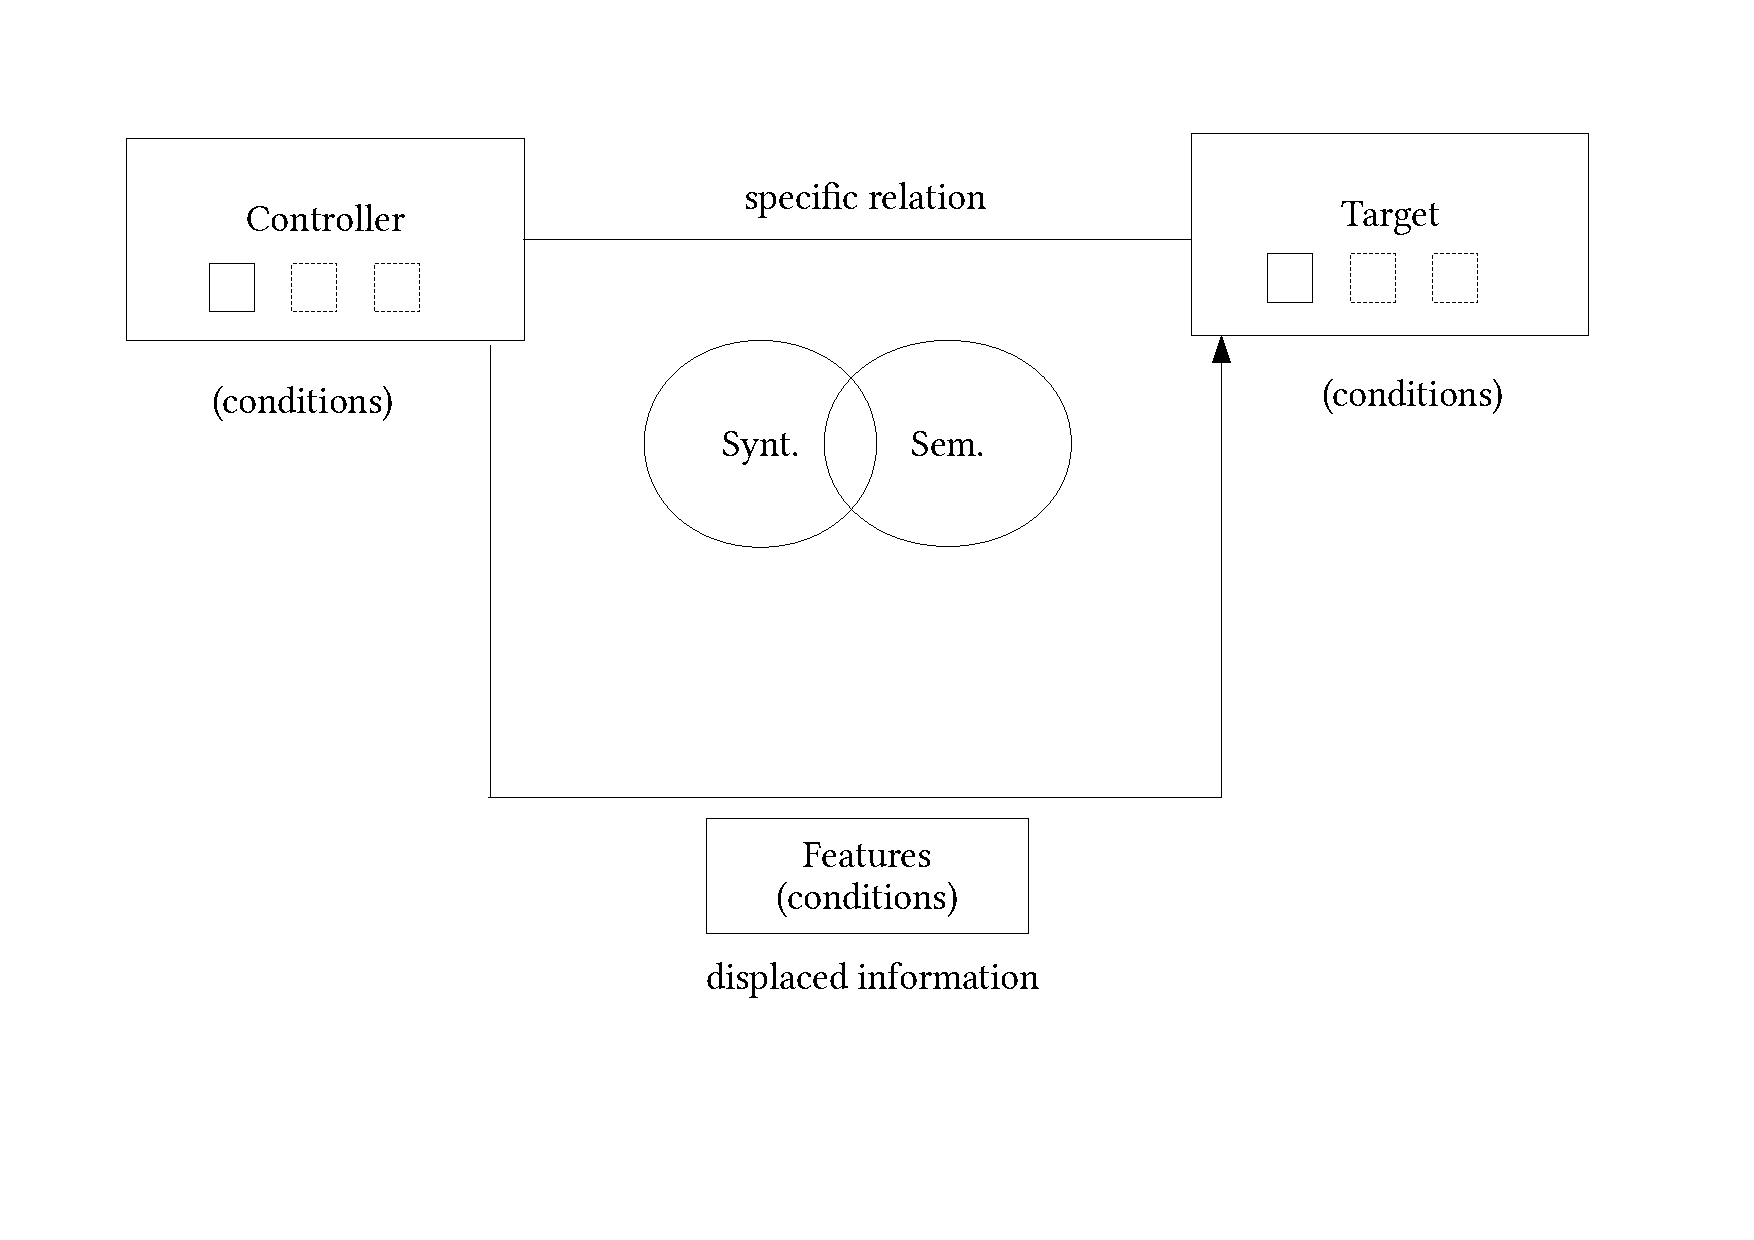
\includegraphics[width=\textwidth]{figures/14/fig3}
\label{fig:WDG:3}
\end{figure}

The visualization in \figref{fig:WDG:3} captures some core ideas of our definition of agreement. Controller and target can consist of several words (small boxes within a larger box). They are linked by a specific relation, which can be syntactic or semantic, and the information expressed by agreement and realized on the target is displaced information, in the sense that it does not originate in the target. It can consist of features or a feature or a condition on a feature.

Unlike Corbett, we think that the notion of relation is an indispensable defining term of agreement. Our definition is consistent in this respect with Lehmann, who requests ``a grammatical or semantic syntagmatic relation'' between controller and target (\citealt[203]{Lehmann1982}). However, we think it need not be syntagmatic, since the controller can be contextual. Coreferentiality is an example of a specific relationship that can hold between a controller and a target. Our claim is that there is always some specific relationship between target and controller in agreement. The relationship must be specific, because it must be unequivocal. This does not exclude occasional instances of ambiguity, but agreement is basically a one-to-one relationship or association, not a one-to-many or many-to-many relationship between controller and target. This entails that targets are sometimes complex in the sense that they consist of \spterm{formal groups}, a term that we take from Croft's (\citeyear[190]{Croft2001}) critique of the notion of constituent. A formal group can be a phrase or constituent, but it can also be another kind of syntactic grouping (which need not be a continuous string of words). Agreement is a means of indicating syntactic grouping (groups of controller and target or target groups or controller groups) parallel to, but not necessarily congruent with, constituency.

Sometimes a word displaying an agreement marker does not entertain any specific or exclusive relation with the controller if considered in isolation, but only when considered in terms of a formal group it is part of. This is evidence for syntactically complex targets. Consider (\ref{ex:WDG:44}) from \ili{Italian} with object agreement in the participle of \textit{dovere} `must' in the verbal formal group \textit{ho dovuti chiudere} `had to close' preceded by the object clitic which triggers the agreement. The object is semantically an object of the verb \textit{chiudere} `to close', but the whole sequence consisting of three verbs is a unit when it comes to argument structure. In terms of \cite{Rizzi1982}, the modal auxiliary and the lexical verb form a verbal complex. As further elaborated in \sectref{sec:WDG:7.4}, the verbal complex in (\ref{ex:WDG:44}) is an instance of a complex target or target group. The clitic, which is coreferential with `pralines and biscuits' in (\ref{ex:WDG:44}), is an object of the whole verbal complex, not just of `must', and as an object of the whole verbal expression it triggers object agreement, which happens to be realized on the modal verb, because the participle is the only form in the verbal complex where object agreement can be realized. Furthermore, \textit{[q]ueste praline e questi biscotti} `these pralines and biscuits' is an instance of a complex controller with gender resolution (in \ili{Italian} feminine and masculine is masculine); see \sectref{sec:WDG:7.3} for complex controllers.

\protectedex{%
\ea\label{ex:WDG:44}
\ili{Italian} (\ili{Indo-European}; \ili{Romance}; constructed, with inspiration of text examples)\\
\gll Queste	praline	e	questi	biscotti	li	ho dovut\textbf{i}	letteralmente	chiudere	sotto	chiave.\\
this.\textsc{f.pl}	praline(\textsc{f}).\textsc{pl}	and	this.\textsc{m.pl}	biscuits\textsc{(m).pl}	3\textsc{m.pl.acc}	have.\textsc{prs.1sg} must.\textsc{ptcp.pst}.\textbf{\textsc{m.pl}}	literal.\textsc{adv}	close.\textsc{inf}	under	key(\textsc{m}).\textsc{sg}\\
\glt `Those pralines and biscuits I had to keep literally under lock and key.'\\
\z
}%

The agreement patterns in (\ref{ex:WDG:44}) can be described as an \spterm{information transfer chain} (see \citealt{Waelchli2018}) consisting of at least ten steps: The masculine plural marker \textit{-i} (i) on the target word \textit{dovuti} (ii) is part of the target group \textit{dovuti chiudere} (iii), which receives masculine plural agreement from the pronoun \textit{li} (iv), serving as controller under the condition that it precedes the verb (cf.\ \textit{ho dovuto chiuder-li}, when the object clitic follows the verbal complex) (v), and is itself a target controlled by the controller group \textit{queste praline e questi biscotti} (vi), whose gender results from gender resolution between the word-forms \textit{praline} and \textit{biscotti} (vii), whose word-form values feminine plural and masculine plural (viii) result from number inflection of the feminine lexeme \textit{pralina} and the masculine noun \textit{biscotto} (xi), which receive their lexical gender by formal gender assignment (x).

Above we have said that the specific relationship can be of different kinds. This is the topic of the next subsection.

  \subsection{Specific relationships in agreement}
\label{sec:WDG:7.2}

It is not the purpose of this section to give an exhaustive treatment of all possible specific relationships that can hold in agreement. What we want to point out here is that coreference is not the only kind of specific relationship that can hold in agreement and that a specific relationship can be semantic (in that case agreement can be inter-sentential) or formal (in that case agreement is usually intra-sentential). The latter part of this section will be devoted to adjacency, which is an under-researched phenomenon often encountered in agreement. We will argue that adjacency may qualify as a specific relationship in agreement.

The clearest case of agreement blatantly violating Moravcsik's (\citeyear[363]{Moravcsik1978}) Coreferentiality Principle is gender in \ili{Archi} (\ili{Nakh-Daghestanian}, \ili{Lezgic}). \ili{Archi} has excessive agreement in the clause with the absolutive argument as controller. In (\ref{ex:WDG:45}) not only the verb `make' agrees with the absolutive argument of the clause, but the pronominal arguments in the ergative and dative cases and the adverb `quickly' do so too.

\ea\label{ex:WDG:45}
\ili{Archi} (\ili{Nakh-Daghestanian}, \ili{Lezgic}; \citealt[3]{Bond2016})\\
\gll Nena<\textbf{b}>u	do:ˁzu-\textbf{b}	χˁon \textbf{b}-ela<\textbf{b}>u	dit:a<\textbf{b}>u	χir	a<\textbf{b}>u\\
\textsc{1pl.incl.erg}<\textbf{\textsc{iii.sg}}>	be.big.\textsc{attr}-\textbf{\textsc{iii.sg}}	cow(\textsc{iii})[\textsc{sg.abs}] \textbf{\textsc{iii.sg}}-\textsc{1pl.incl-dat}<\textbf{\textsc{iii.sg}}>	quickly<\textbf{\textsc{iii.sg}}>	behind	<\textbf{\textsc{iii.sg}}>make.\textsc{pfv} \\
\glt `We quickly drove the big cow to us (home).'\\
\z

In our view, agreement here marks the whole clause as a formal group; put differently, the agreement target is the whole clause (see \sectref{sec:WDG:7.4} for complex targets). Agreement with the same noun class is realized wherever it can be morphologically marked in the clause. This is actually less excessive in \ili{Archi} than (\ref{ex:WDG:45}) suggests, because agreement can be spelled out only occasionally in the \ili{Archi} clause. Agreement appears only in about one third of the verbs, in the ergative only in the inclusive plural, in the dative only in first person pronouns, and only in 13 of 392 adverbs (\citealt[70]{Bond2016}). In clauses with two verbs with different absolutives, so-called biabsolutive constructions, there are two formal groups for agreement (\citealt[90--111]{Chumakina2016}).

The agreement relation in \ili{Archi} is a specific relationship in the sense that it is a unique relationship between the head of the absolutive NP (controller) and its clause (target). Since this is a syntactic dependency relationship, \ili{Archi} agreement is intra-sentential, as opposed to coreference, which is semantic and can be inter-sentential. However, coreference is not the only possible kind of specific semantic relationship in agreement.

\spterm{co-conceptuality} \textendash{} where controller and target express identity of concept, but not identity of reference \textendash{} is another important specific relationship in gender agreement. Unlike co-referentiality, there is usually no agreement in number, since number is a property of the referent, not of the lexical noun expressing the concept (except for pluralia tantum, see \citealt{Waelchli2017} for \ili{Latvian}). If we consider examples from the literature on anaphoric pronouns without explicit antecedents, such as \textit{Either no letter was sent, or \textbf{it} got lost} and \textit{Watch out for that snake. \textbf{They} are poisonous} (\citealt[211]{Bosch1988}), there is no relationship of co-reference between noun and pronoun. The anaphoric pronoun simply stands for something that is of the same kind as the noun (the same concept); \textit{it} is a letter and \textit{they} are snakes, irrespective of their reference and whether they are referential at all. The so-called ``donkey sentences'' also sort here. This term was first introduced by the medieval philosopher Walter Burleigh around 1328 based on the \ili{Latin} \textit{Omnis homo habens \textbf{asinum}} [donkey.\textsc{acc.sg.m}] \textit{videt illum} [\textsc{dem.acc.sg.m}] `Every man having a donkey sees it' (\citealt[269]{Seuren2009}). In languages with lexical gender, such as \ili{Latin}, there is usually agreement in gender in such cases of co-conceptuality.

Co-conceptuality is particularly important for independent adjectives and numerals and other independent elements as was discussed in \sectref{sec:WDG:4}. Like anaphoric pronouns, independent adjectives typically express some sort of anaphoric relationship, which, however, does not imply identity of reference, but identity of concept. This is illustrated in (\ref{ex:WDG:46}) from \ili{German}.

\ea\label{ex:WDG:46}
\ili{German} (\ili{Indo-European}, \ili{Germanic}): independent adjective expressing co-conceptuality\\
\textit{Das mit dem \uline{Hemd}} [shirt(\textsc{n})] \textit{leuchtet mir so langsam auch ein... ja, \textbf{ein weißes}} [\textsc{indf.nom.sg.n} white.\textsc{nom.sg.n}] \textit{wäre in der \ili{Tat} besser gewesen.}\\
{[}After a non-successful job application:{]} `The thing with the shirt starts becoming clear to me, too...yes, a white one would indeed have been better.'\\
http://www.bewerbung-forum.de [2018-11-06] \\
\z

\newpage 
It might be objected that (\ref{ex:WDG:46}) is a case of ellipsis of the head noun. However, the form of attributive adjectives or numerals with head nouns and of independent adjectives or numerals without head nouns is not always the same in all languages, which is an argument that independent adjectives and numerals are not attributive adjectives and numerals with ellipsis. In \ili{German}, the independent numeral `one' follows a different declension pattern (originally pronominal endings): (speaking of shirts) \textit{ein-\textbf{es} ist hellgrau} [one-\textsc{nom.sg.n.pron} be.\textsc{prs.3sg} light.gray] `one is light gray' as opposed to \textit{ein Hemd ist hellgrau} [one.\textsc{nom.sg.n} shirt be.\textsc{prs.3sg} light.gray] `one shirt is light gray'. \cite{Waelchli2017} discusses the case of Dundaga Latvian,\il{Latvian, Dundaga} where there is gender agreement only in NPs with head nouns, but not in independent adjectives (which only have number agreement; see example (\ref{ex:WDG:31}) in \sectref{sec:WDG:4.4}). As far as the Animacy Hierarchy is concerned, independent adjectives behave like pronouns. In (\ref{ex:WDG:47}) from \ili{German} there is semantic (referent-based) agreement with independent adjectives rather than lexical agreement. With attributive adjectives, semantic agreement is ungrammatical (\textit{das}[\textsc{n}] \textit{ältere Mädchen}(\textsc{n}), \textit{*die}[\textsc{f}] \textit{ältere Mädchen}(\textsc{n}) `the older girl').

\ea\label{ex:WDG:47}
\ili{German} (\ili{Indo-European}, \ili{Germanic}): co-conceptuality linked to coreference by means of part-whole relationship\\
\textit{\uline{Zwei Mädchen}} [girl\textsc{(n).pl}] \textit{im Alter von sieben und acht Jahren sind am Samstag in Schwarzenberg am Böhmerwald (Bezirk Rohrbach) von der Holzleiter eines Hochstandes gestürzt. \textbf{Die}} [\textsc{def.nom.sg.f}] \textit{\textbf{ältere} der beiden war ausgerutscht und hatte \textbf{die}} [\textsc{def.acc.sg.f}] \textit{\textbf{jüngere} mitgerissen.}\\
	`Two girls aged seven and eight years fell from the wooden ladder of a tree stand in Schwarzenberg am Böhmerwald (district of Rohrbach) on Saturday. \textbf{The elder one} of the two had slipped and had dragged \textbf{the younger one} with her.' \url{http://www.salzburg.com/nachrichten/oesterreich/chronik/sn/artikel/zwei-maedchen-in-ooe-von-hochstand-gestuerzt-und-verletzt-209318} [accessed 2017-06-05]\\
  \z

In the rest of this section we will focus on adjacency as a further potential specific relationship in agreement.

\spterm{adjacency} in agreement means that controller and target or target and controller immediately follow each other. Target and/or controller can consist of several words. Adjacency between controller and target is frequent in most languages with gender, which is natural, since agreement is often local. According to \cite{Corbett2006}, local agreement is more canonical than distal agreement. But most treatments of gender do not pay any particular attention to adjacency. We think that adjacency is an important issue in agreement that deserves particular attention because there are several languages where gender agreement is predominantly or exclusively adjacent.

Since adjacency is unequivocal, it has the potential of qualifying as a specific relationship between controller and target. Thus, it is a candidate for a type of specific relationship between controller and target on a par with coreference and other specific relationships.

It is well-known that linearity plays an important role in phonology, notably in sandhi phenomena, sound changes that take place at word- or morpheme-boundaries. As already mentioned in \sectref{sec:WDG:6.4}, some instances of gender agreement originate in sandhi. This adds a developmental perspective to the study of adjacency in gender agreement. In cases where sandhi is involved in the origin of gender agreement, adjacency may reflect preservation of an earlier phonological motivation.

The importance of sandhi phenomena in agreement is well-known from \ili{Celtic} languages. In all \ili{Celtic} languages, feminine nouns have ``mutated'' onsets following an article: \ili{Irish} \textit{bean} `woman(\textsc{f})', \textit{an bhean} `the woman'; \ili{Welsh} \textit{pont} `bridge(\textsc{f})', \textit{y bont} `the bridge' (\citealt[480]{Fife1998}). Here it looks as if the controller noun is at the same time the target. However, morpho-syntactically it is rather the article which is the target with the gender marker being realized phonologically on the following word. In the case of postposed adjectives, it is just the other way round. In \ili{Breton} \textit{ur verc'h vras} `a big girl' (\textit{merc'h} `girl', \textit{bras} `big'), \textit{vras} `big' looks as if it displays agreement with its initial mutation, but the mutation is in fact diachronically caused by the feminine noun preceding it (\citealt[480]{Fife1998}). (For the possessive pronoun in \ili{Welsh} see \citealtv{Waelchlithisyear}.)

Let us now turn to the discussion of languages in which target and controller in gender agreement almost always are adjacent. In \ili{Uduk}, a language with two noun classes termed class 1 and class 2, gender targets immediately precede gender controllers (see \citealtvo{Killianthisyear}). At the same time, coreference does not seem to play any major role. If there are two or more words in a noun phrase, the head noun and the modifier have genders of their own.%
\footnote{%
For one single exception involving prenominal modifiers, see \cite[128]{Killian2015}.
} %
Gender in \ili{Uduk} does not usually have the function of signaling that two words belong to the same constituent or are coreferential. The gender marker is simply triggered by the gender of the following word. In (\ref{ex:WDG:48}) the preposition \textit{kí} is followed by a class 1 noun (\textit{yìl} `year'). With a following class 2 noun it would be \textit{ká}. The modifier `small', however, is class 2, as are all modifiers derived from stative verbs with the suffix \textit{-gàʔ}. This is why the associative marker, which links words in the NP, takes a class 2 marker. Since the gender markers are clitics in some case forms (see \citealtvo{Killianthisyear}), the words on which the gender marker may appear make sometimes rather unexpected targets, such as the adverbial subordinator \textit{gòm} in (\ref{ex:WDG:48}).

\ea\label{ex:WDG:48}
\ili{Uduk} (\ili{Koman}; \citealt[382]{Killian2015})\\
\gll gòm=\textbf{à}	'cí	yĭsā̀	ʼbór-óʼd	áʼdī	kí	màsh	kī-Ø	yìl=à	gwăʼd-gàʔ\\
 for=\textbf{\textsc{cl2}}	ʼchild(\textbf{\textsc{cl2}})	\textsc{neg}	good:\textsc{ipfv-3sg}	\textsc{3sg}	\textsc{narr}	marry	with-\textbf{\textsc{cl1}}	year(\textbf{\textsc{cl1}})=\textsc{ass.cl2}	small-\textsc{nmlz(cl2)}\\
\glt `Because it's not good for the child to marry early.' \\
\z

\noindent It is not entirely obvious what the target is in this case. In one possible analysis, \textit{gòm} is the gender target, because this word bears the gender marker. In another possible analysis, which we prefer, the gender target is the clitic \textit{=à} which happens to require a host for phonological rather than morphosyntactic reasons.

While almost all gender agreement in \ili{Uduk} is adjacent, the \ili{Taa} languages \ili{West ǃXõo} [=\ili{West Xoon}] and \ili{East ǃXõo} [=\ili{East Taa}] (\ili{Tuu} [=Southern \ili{Khoisan}], \ili{Taa}) have several different kinds of agreement, only one of which exhibits adjacency. Agreement preceding the controller is necessarily adjacent, agreement within the NP with the NP head noun as controller is not. Adjacency agreement is illustrated in (\ref{ex:WDG:49}) with a compound. Its first part, which is not the head of the compound, triggers agreement on the preceding word. In \ili{Taa} languages, the gender of the whole compound often differs from the gender of the parts of the compound. In (\ref{ex:WDG:49}), \textit{ǁkx'oe nǁaen} [rain house.\textsc{pl}] `clouds' has gender \textsc{cl2a[sg]/cl2a[pl]}, but \textit{ǁkx'oe} `rain' (only singular) has gender 3 and \textit{nǁahe} \textsc{sg} (\textit{nǁaen} \textsc{pl}) `house' has gender \textsc{cl3[sg]/cl1[pl]}. Adjacent gender in \ili{Taa} languages is always controlled by the immediately following noun, which is the first part of the compound, \textit{ǁkx'oe} `rain(\textsc{cl3})' in (\ref{ex:WDG:49}), rather than the whole compound `cloud(\textsc{cl2a})'. In (\ref{ex:WDG:50}), there is an associative plural formed from a person name. The associative plural has gender 4. However, the adjacency agreement is triggered by the gender of the person name, which is gender 1.
\largerpage

% \protectedex{%
\ea\label{ex:WDG:49}
\ili{West ǃXõo} (\ili{Tuu}, \ili{Taa}; \citealt{Gueldemann2004}): adjacency and compound gender\\
\gll n 	si 	nǀa=\textbf{e} 	ǁkx'oe	nǁaen 	ka 	ǁari 	ka\\
\textsc{1sg} 	\textsc{ipfv} 	see=\textbf{\textsc{cl3}} 	[rain(\textbf{\textsc{cl3}}) 	house.\textsc{pl(cl1)](cl2a)} 	\textsc{rel.cl2a}	many 	\textsc{rel.cl2a}\\
\glt `I see many clouds.'\\
\z
% }%

\ea\label{ex:WDG:50}
\ili{West ǃXõo} (\ili{Tuu}, \ili{Taa}; \citealt{Gueldemann2006}): adjacency and associative plural\\
\gll nna	nǀa=\textbf{i}	Tom-tu	ku	ǀai	k=i	dertien	ku\\
\textsc{1sg:prf}	see=\textbf{\textsc{cl1}}	[Tom(\textbf{\textsc{cl1}})-\textsc{ass.pl](cl4)}	\textsc{rel.cl4}	stay	\textsc{oblique=cl1}	\textsc{toponym(cl1)}	\textsc{rel.cl4}\\
\glt `I have seen Tom and them who were at post 13.'\\
\z

Some clitic hosts, such as the question particle \textit{ǀV} in (\ref{ex:WDG:51}) (\textit{V} means that the vowel must come from agreement), never occur without a following gender clitic. There is thus no gender marking, if there is no clitic host. If (\ref{ex:WDG:51}) were not a question, there would not be any gender marker.

\ea\label{ex:WDG:51}
\ili{East ǃXõo} (\ili{Tuu}, \ili{Taa}; \citealt[18]{Traill1994})\\
\gll	ǀ=\textbf{ú}	tûu	à	sîl\\
	\textsc{q=\textbf{cl4}}	people(\textbf{\textsc{cl4}})	\textsc{tense}	come\\
\glt	`Did the people come?'\\
\z


A third language where adjacency plays an important role is \ili{Nalca}. Gender is triggered by the immediately preceding constituent. In (\ref{ex:WDG:52}) the noun \textit{heik} `hamlet' is followed by two case markers, dative plus comitative, which together express the notion of source. Case markers and gender markers are mutually dependent on each other and hence almost always co-occur in the case-number word following the noun. In (\ref{ex:WDG:52}), \textit{heik} `hamlet' is default noun \textit{e}-gender, which is why the first case-number word in (\ref{ex:WDG:52}) is default noun \textit{e}-gender. However, since the controller cannot control anything but the gender of the immediately following target, the second case-gender word is default phrase \textit{a}-gender (which is never triggered by a lexical noun). There is no adjacency condition on the demonstrative suffix, which is repeated in both case-number words.

\protectedex{%
\ea\label{ex:WDG:52}
\ili{Nalca} (Nuclear \ili{Trans-New Guinea}, \ili{Mek}; New Testament 40021001; \citealt{Waelchli2018})\\
\gll Heik	e-\textbf{nye}-k	a-\textbf{nye}-b	dara\\
hamlet	\textsc{dn-\textbf{dem}-dat}	\textsc{dp-\textbf{dem}-com/abl}	\textsc{top}\\
\glt `from this hamlet'\\
\z
}%

As argued by \cite{Waelchli2018}, gender in \ili{Nalca} partly derives from sandhi phenomena, which motivates adjacency diachronically.

In both \ili{Nalca} and \ili{Uduk}, person names are important gender controllers (see \citealtvo{Killianthisyear} for \ili{Uduk}). In the \ili{Oceanic} languages spoken on the island of Makira, gender classes have developed from an extension of person name markers, and, as discussed in \sectref{sec:WDG:6.4}, one of five classes in \ili{Owa} originates from sandhi phenomena. Person names rarely have attributes. Thus it is natural that person name markers and person names are typically adjacent.

Adjacency-based gender developing from person name markers is not particularly complex when it first develops. There is only one agreement target, person name markers, and gender need not be specified in the noun lexicon, since it is organized by the animacy hierarchy (see \sectref{sec:WDG:3}). Person name markers can then travel down the animacy hierarchy, first expanding to older kinship terms and to other words typically expressing unique reference, in \ili{Makira languages} also to the pronoun `who'. Both \ili{Mek} languages and \ili{Makira languages} illustrate complexification in terms of number of classes (in \ili{Mek} from two in \ili{Una} and \ili{Eipo} to four to six in \ili{Nalca}, depending on whether only classes with lexical controllers or all classes are counted, and in Makira from two in \ili{Arosi} to four in \ili{Kahua} and five in \ili{Owa}). \ili{Uduk} gender is considerably more complex in terms of gender assignment (see \citealtvo{Killianthisyear}) and it is not known how the system has developed. Gender in \ili{Taa} languages is the most complex among the languages discussed here and nothing is known about the origin of the system.

  \subsection{Complex controllers}
\label{sec:WDG:7.3}

Complex controllers, where the controller consists of more than one word, are well-known from gender resolution in coordination, but also inalienable possession, names consisting of several words, and nominalizations. They provide evidence for gender being assigned to a group of words rather than to a single word. In this section we will consider evidence from inalienable possession in \ili{Paumari}, from \ili{German} restaurant names and \ili{Taa} nominalizations. The section also discusses \ili{Nalca}, where complex controllers are pervasive.

The assumption of complex controllers is uncontroversial for gender resolution in coordination, as illustrated in (\ref{ex:WDG:44}) in \sectref{sec:WDG:7.1}. However, gender resolution is not restricted to coordination. Consider (\ref{ex:WDG:53}) from \ili{Paumari}, a language with two different gender systems: masculine/feminine and \textit{ka-} vs.\ non-\textit{ka}-noun classes. In \ili{Paumari}, there is gender resolution in inalienable possession in the \textit{ka-} vs.\ non-\textit{ka} gender system. ``If either the possessor, or the possessed noun (or both) belong to the \textit{ka-} class, a modifier takes the \textit{ka-} class marking, no matter which one of the two it modifies'' (\citealt[240]{Aikhenvald2010}). Put differently, \textit{ka-}/non-\textit{ka} gender in \ili{Paumari} inalienable possession is computed with formal criteria in the same way as in gender resolution in coordination. In (\ref{ex:WDG:53}) the possessor is \textit{ka} and the possessed noun is non-\textit{ka}. The adjective displays \textit{ka}-agreement whether it modifies the possessor or the possessed noun.%
\footnote{%
For similar phenomena in the related language \ili{Jarawara}, where the \textit{ka}/non-\textit{ka}-gender was lost, see \cite{Dixon2000} and \sectref{sec:WDG:3.4}.
} %
The possessor \textit{bodi} `mouth(\textsc{n.\textit{ka};f})' also takes \textit{ka-} because it agrees with \textit{ojoro} `turtle(\textsc{\textit{ka};f})'.

\ea\label{ex:WDG:53}
\ili{Paumari} (\ili{Arawan}, \citealt[240]{Aikhenvald2010}): gender resolution in inalienable possession\\
\gll	ojoro	ka-bodi-ni	\textbf{ka}-karaho\\
	turtle(\textsc{\textit{ka};f})	\textsc{\textit{ka}}-mouth(\textsc{n.\textit{ka};f})-\textsc{3sg.f.deriv}	\textbf{\textit{\textsc{ka}}}-big\\
\glt `big mouth of a turtle' or `mouth of a big turtle'\\
\z

Further evidence for complex controllers comes from cases where gender is assigned on the level of group of words rather than on the level of words, which can hold for names consisting of several words. \cite{Plank2015} discusses \ili{German} restaurant names, which often can be neuter irrespective of the gender of the head noun.%
\footnote{%
According to \cite{Plank2015}, recategorization with default-neuter for \ili{German} restaurants pragmatically indicates the distance of the name to gastronomy. Traditional names for restaurants, such as \textit{Die Sonne} [the.\textsc{f} sun(\textsc{f})] and \textit{der Ratskeller} [the.\textsc{m} council.cellar(\textsc{m})] are not neuter. Neuter gender for \ili{German} restaurants is not obligatory.
} %
The \ili{German} lexeme \textit{Orkan} `hurricane' is masculine. However, in (\ref{ex:WDG:54}), \textit{Orkan} is used as name for a restaurant and is neuter. (\ref{ex:WDG:55}) illustrates the same phenomenon with a name consisting of more than one word. \textit{Oma} `grandma' is feminine, but it is the whole expression \textit{Oma Plüsch} `grandma Plush' that is the restaurant name and as a restaurant name consisting of two words it is neuter.

\protectedex{%
\ea\label{ex:WDG:54}
\ili{German} (\ili{Indo-European}, \ili{Germanic}; \citealt[132]{Angerer2009})\\
\gll Hinter	der	wohl	schmalsten	Eingangstüre Regensburgs	verbirgt	sich	\textbf{das}	Orkan.\\
behind	\textsc{def.gen.sg.f}	probably	narrow.\textsc{superl.gen.sg.f}	entrance.door(\textsc{f}) Regensburg.\textsc{gen}	hide.\textsc{prs.3sg}	\textsc{rfl}	\textbf{\textsc{def.nom.sg.n}}	hurricane(\textsc{m})\\
\glt `The Orkan is hidden behind the probably narrowest door in Regensburg.'\\
\z
}%

\protectedex{%
\ea\label{ex:WDG:55}
\ili{German} (\ili{Indo-European}, \ili{Germanic}; tripadvisor.de [2018])\\
\gll \textbf{Das}	Oma	Plüsch	liegt	direkt	an	der	Donau.\\
\textbf{\textsc{def.nom.sg.n}}	grandma(\textsc{f})	Plüsch	lie.\textsc{prs.3sg}	directly	at	\textsc{def.dat.sg.f}	Danube(\textsc{f})\\
\glt `Oma Plüsch is located directly at the River Danube.'\\
\z
}%

Adjectives as parts of names commit restaurant names to the gender of their lexical head: \textit{der Bayerische Bahnhof} [the.\textsc{m.sg} Bavarian.\textsc{m/f/n.sg} railway\_station(\textsc{m})], even if the adjective cannot inflect: \textit{die Schweizer Grenze} [the.\textsc{f.sg} Swiss.\textsc{adj} border(\textsc{f})]. This only holds if the adjective is part of the name. With non-restrictive adjectives neuter is possible: \textit{das spießige Vier Jahreszeiten} [the.\textsc{n.sg} petty-bourgeois.\textsc{m/f/n.sg} four seasons.\textsc{pl}] (\citealt{Plank2015}). To state this in more general terms, if the lexical head is already combined with a potential target before the name is completed, the noun phrase has already committed itself to a gender, thus gender assigned to the name as a whole is no longer available. The same rule holds, for instance, for names of roses, which can be default-feminine unless they contain an adjective (\textit{die Helmut Schmidt}, \textit{die Gruß an Helgoland} [the.\textsc{f.sg} greeting(\textsc{m.sg}) to Helgoland], but \textit{der Gelbe Engel} [the.\textsc{m.sg} yellow angel(\textsc{m})]).%
\footnote{%
Sometimes the gender of names is paradigmatically inherited \textendash{} names of roses (\textsc{f}), apples (\textsc{m}), pears (\textsc{f}), beers (\textsc{n}), and wines (\textsc{m}) have the gender of their general noun as default. However, in case of restaurants (\textsc{n}), ships (\textsc{f}), motorcycles (\textsc{f}), and cars (\textsc{m}), the default-gender is not inherited from a general noun.
} %

While complex controllers in \ili{German} are limited to names, \ili{Nalca} has them all over. In \ili{Nalca} there is a general alternation between one of four lexical genders \textendash{} masculine \textit{be-}, feminine \textit{ge-}, phonologically assigned CV-gender \textit{ne-} (the controller has the structure CV or V), and default noun \textit{e}-gender \textendash{} and default phrasal gender \textit{a-}, which is never controlled by a lexical noun. The switch is syntactically determined. Having certain modifiers (``allies'') helps the noun impose its lexical gender, having certain other modifiers (``obstacles'') conditions the phrasal default. Most nouns cannot impose their lexical gender unless they have an attribute ally that helps them impose their gender, as in (\ref{ex:WDG:56}) about boys' initiation rites, where \textit{me} `boy, child' with lexical CV-gender \textit{ne-} triggers \textit{ne-} only if there is an adjective in the NP, but has default phrase \textit{a-} if it is bare in the NP.

\ea\label{ex:WDG:56}
\ili{Nalca} (Nuclear \ili{Trans-New Guinea}, \ili{Mek}; \citealt{Binzellnd}{}; \citealt[71]{Waelchli2018})\\
\gll \uline{me}	\textbf{a-ra}	gɛlɛlinga	sɔob-vka	bɔ-ba-lam-ek. \uline{Nauba}	\uline{me}	\textbf{ne-ra}	al-biyok	ba-lam-ok.	\uline{Mek}	\uline{me}	\textbf{ne-ra}	sɔob-oka	bɔ-ba-lam-ek.\\
child(\textsc{cv})	\textbf{\textsc{dp-top}}	unnoticed	enclose.in.netbag-\textsc{cvb}	carry-go-\textsc{hab/ipfv-pst.3pl} big	child(\textsc{cv})	\textbf{\textsc{cv-top}}	\textsc{3sg}-alone	go-\textsc{ipfv-pst.3sg} small	child(\textsc{cv})	\textbf{\textsc{cv-top}}	enclose.in.netbag-\textsc{cvb}	carry-go-\textsc{hab/ipfv-pst.3pl}\\
\glt `They carried the boy away secretly in a netbag. A big boy went by himself. A small boy they carried in a netbag.'\\
\z

There is a parallel in Mopán Maya,\il{Maya, Mopán} where gender also has developed from an extension of person name markers. Gender in Mopán Maya\il{Maya, Mopán} is marked only on one target, the ``gender marker'' proposed to the noun or adjective+noun, which distinguishes masculine \textit{aj} and feminine \textit{ix} (\citealt{Contini-Morava2018}). Only a minority of nouns have gender, most nouns take the article \textit{a} instead (which, unlike gender markers, is not compatible with possessive pronouns). Nouns that are not gendered when used in isolation may sometimes optionally have a gender marker if there is an attributive adjective. \cite[138]{Contini-Morava2018} give an example from a story where \textit{a ch\textquotesingle{}o\textquotesingle{}oj=o} [\textsc{art} rat=\textsc{echo}] `rat' is first introduced without gender and then occurs with adjectives and gender markers as \textit{aj noxi\textquotesingle{}  ch\textquotesingle{}o\textquotesingle{}oj=o} [\textsc{gm.m} big rat=\textsc{echo}] and \textit{aj tz\textquotesingle{}i\textquotesingle{} ch\textquotesingle{}o\textquotesingle{}oj=o} [\textsc{gm.m} small rat=\textsc{echo}] with a gender switch very similar to that in the \ili{Nalca} example (\ref{ex:WDG:56}). The difference is that \ili{Nalca} \textit{a-} default phrase gender is formally integrated in the gender system and the alternation is more systematic in \ili{Nalca}.

\largerpage
In some languages, sentential nominalizations can be gender controllers. \ili{Nalca} sentential nominalizations, if not followed by a noun, can take one of three phrasal suffixes and each of the three resulting constructions without a nominal head takes another gender. Two of the three suffixes are homonymous and are distinguished only by the gender they control (\citealt{Waelchli2018}): male nominalizations with suffix \textit{-nya} (\ref{ex:WDG:57}) take masculine gender \textit{be-} and thing-nominalizations with suffix \textit{-nya} (\ref{ex:WDG:58}) take neuter gender \textit{ne-} (which happens to have the same form as CV-gender in (\ref{ex:WDG:56})).

\ea\label{ex:WDG:57}
\ili{Nalca} (Nuclear \ili{Trans-New Guinea}, \ili{Mek}; New Testament, 44010021; \citealt[80]{Waelchli2018})\\
\gll {...} [ugun-da	na	e-le-nu-lum]-\textbf{nya}	\textbf{be}-ra,	na-ra	al-an ...\\
{} \textsc{2pl-top}	\textsc{1sg}\footnotemark{} 	search-\textsc{ipfv-obj.1sg-prs.2pl-\textbf{nmlz.m}}	\textbf{\textsc{m-top}}	\textsc{1sg-top}	\textsc{3sg-dem} {}\\
\glt `...I am he whom you are looking for!', lit.\ `I am he, the one [you are looking for me]'\\
\z
%
\footnotetext{In \ili{Nalca} nominalizations, O is often zero marked, but `thing' nominalizations tend to have a dative-marked O as in (\ref{ex:WDG:58}).}

\ea\label{ex:WDG:58}
\ili{Nalca} (Nuclear \ili{Trans-New Guinea}, \ili{Mek}; New Testament, 43006026; \citealt[80]{Waelchli2018})\\
\gll {...} [ugun-da	na-k	e-le-nu-lum]-\textbf{nya}	\textbf{ne}-ne-ra {...}\\
{} \textsc{2pl-top}	\textsc{1sg-dat}	search-\textsc{ipfv-obj.1sg-prs.2pl-\textbf{nmlz.n}}	\textsc{\textbf{n}-dem-top} {}\\
\glt `...you seek me not [because you saw signs]...', lit.\ `this fact that [you are looking for me]' \\
\z

\ili{Nalca} nominalizations are morphologically marked, but there is also a semantic component, which is strengthened by the homonymy of two different morphological markers. There is no competition with lexical gender as there are no lexical heads in the construction. The sentential nominalization with its morphological marker must immediately precede the gender target (adjacency agreement, see \sectref{sec:WDG:7.2}).

A similar construction is found in \ili{East ǃXõo}, where, however, nominalizations can only take one gender. The nominalization suffix \textit{-sà} can attach to the verb stem (\textit{!qāhe-sà} [hunt-\textsc{nmlz(cl2)}] `hunting') or to a verb phrase, the subject of the nominalization being expressed by a possessor in a \textsc{possessor }\textit{ǀV}+\textsc{gender.marker possessed} construction. The preposition \textit{ǀV} takes the gender of the immediately adjacent following controller. The only available controller is the nominalized verb phrase, which is a constituent without any lexical head from which the gender of the nominalization derives.

\ea\label{ex:WDG:59}
\ili{East ǃXõo} (\ili{Tuu}, \ili{Taa}; \citealt[30]{Traill1994}; \citealt[7]{Gueldemann2004})\\
\gll ùh	ń	bà	ǁṵ̄-n	ǀà	ǀùã	{ǀàũ ǁnàa}	ǀnēe-\textbf{sà}\\
\textsc{cl4}	\textsc{tense}	\textsc{aspect}	refuse-\textsc{1sg}	\textsc{poss.cl2}	hold/give.\textsc{cl2}	tobacco(\textsc{cl2})	to.3-\textbf{\textsc{nmlz(cl2)}}\\
\glt `They disapprove of my giving him tobacco.'\\
\z

To summarize, there is a diverse set of formal syntactic groups that can all function as complex controllers. These include NP-coordination (gender resolution), possessed and possessor in inalienable possession, names consisting of several words, nominalizations, and \textendash{} in \ili{Nalca} \textendash{} any kind of noun phrase. Since compounds are also groups of words, we can also add compounds taking compound gender, as in \ili{Khasi} (see \sectref{sec:WDG:6.3}), as a further type of formal groups serving as complex controllers.

  \subsection{Complex targets}
\label{sec:WDG:7.4}

Target groups or complex targets must be invoked whenever the agreement relation applies between the controller and a formal group of words. This is the case, for instance, if the target is a complex predicate consisting of several verbs (lexical verb and auxiliary) which share the same argument structure. This is most clearly visible if there is agreement with the object and the agreement is realized on an auxiliary as in (\ref{ex:WDG:44}) from \ili{Italian} discussed in \sectref{sec:WDG:7.1}.

\cite{Haspelmath1999} discusses the \ili{Italian} data together with two languages where agreement goes with the absolutive to which we turn now: \ili{Godoberi} (\ili{Nakh-Daghestanian}, Andic) and \ili{Hindi} and \ili{Urdu} (\ili{Indo-European}, \ili{Indo-Aryan}). In (\ref{ex:WDG:60}) from \ili{Hindi}/\ili{Urdu}, the feminine noun `bread' is the object of `eat', but all three verbs in the verb complex display agreement. This means that the three verbs together make up one complex target. (\ref{ex:WDG:61}) from \ili{Godoberi} shows so-called ``long distance agreement'', which \cite{Haspelmath1999} analyzes as an instance of clause-union. In our terms, the four verbs in (\ref{ex:WDG:61}) together constitute a formal group sharing the object argument and are a single complex target, with the neuter plural of the absolutive realized on three of them (`want' never takes agreement).

\ea\label{ex:WDG:60}
\ili{Hindi}/\ili{Urdu} (\ili{Indo-European}, \ili{Indo-Aryan}; \citealt[23]{Wunderlich1994}; \citealt[147]{Haspelmath1999})\\
\gll	Raam	ne	rot̩ii	khaa-n\textbf{ii}	caah-\textbf{ii}	thii.\\
	Ram	\textsc{erg}	bread\textsc{\textbf{(f)}[sg]}	eat-\textsc{inf.\textbf{f.sg}}	want.\textsc{pst-\textbf{f.sg}}	be.\textsc{pst.f.sg}\\
\glt	`Ram had wanted to eat bread.'\\
\z

\ea\label{ex:WDG:61}
\ili{Godoberi} (\ili{Nakh-Daghestanian}, Andic; \citealt[143]{Haspelmath1999})\\
\gll	ilu-ɬi	quči-be	\textbf{r}-al-u	\textbf{r}-uL-i 	q'°araʕ-anta	\textbf{ru}-k'-a.\\
	mother-\textsc{dat}	book\textsc{(n)-pl[abs]}	\textbf{\textsc{pl.n}}-read-\textsc{cvb.pst}	\textbf{\textsc{pl.n}}-finish-\textsc{inf}	want-\textsc{cvb.prs}	\textbf{\textsc{pl.n}}-be-\textsc{aor}\\
\glt 	`Mother wanted to finish reading the books.'\\
\z

\ili{Nakh-Daghestanian} languages are known for their extensive clausal agreement, which takes different forms in different languages. In \ili{Godoberi} all verbs of a unified clause together constitute an agreement target (see also the similar case of \ili{Archi} in \sectref{sec:WDG:7.2}).

Complex gender targets involving complex predicates also occur in \ili{Coastal Marind}. In (\ref{ex:WDG:62}) the patient \textit{ebta} `sago thatch' is an argument of the transitive verb \textit{takun} `make roof', but agreement is shown on the auxiliary \textit{balen} `finish (intr./tr.)'.%
\footnote{%
For similar phenomena involving person in another language in South New Guinea, \ili{Nen} (Morehead-Wasur), see \cite{Evans2015}.
} %

\ea\label{ex:WDG:62}
\ili{Coastal Marind} (\ili{Anim}, Marindic; Bruno Olsson, p.c.)\\
\gll ebta	takun	mbya	nak-ap-ba<\textbf{h}>in	\\
sago.thatch(\textbf{\textsc{iv}})	make.roof	\textsc{neg}	1.\textsc{a-contessive}-finish<\textbf{\textsc{iv.u}}>\\
\glt `I didn't finish making the sago thatch roofing.'\\
\z

In discussing agreement in case, \cite[222]{Lehmann1982} points out that viewing the head noun as controller of agreement is problematic notably when an NP lacks a head noun. This also holds for gender in independent headless NPs, such as \ili{Italian} \textit{Tu sei la più bella} `you are the most beautiful one (\textsc{f})' (see \sectref{sec:WDG:4}). Here it is obviously not the article controlling feminine gender on the adjective or vice versa, but the whole headless noun phrase in the predicate is a target group assigned feminine singular by a latent contextual controller.

If attributes in headless NPs form target groups, the question arises as to whether a series of target words within the same NP could generally be considered to constitute a target group. In many languages gender agreement with multiple targets in an NP is a way to signal that these elements all belong together in one formal group (which can be contiguous or non-contiguous). This would then mean that in NP agreement the head noun is the controller and the whole NP is the target. A potential problem is then that the head noun controlling the NP is also part of the NP. \cite[223]{Lehmann1982} suggests that this could be solved with the following condition ``If B is the head of an NP A, B is not said to agree.'' This may seem entirely ad hoc at first glance. However, if we take into account that agreement is displaced information, it is a priori excluded that the controller can be part of the target. Target groups are formal groups, but not all formal groups are syntactic constituents. The easiest solution is to say that in NP agreement, the target group is the NP minus the head noun. What we have said for NPs here also applies to clauses in the \ili{Daghestanian} languages \ili{Archi} and \ili{Godoberi} where the whole clause can be the agreement target (see \sectref{sec:WDG:7.2}).

A further case of complex targets are gendered clauses in \ili{Ngan\textquotesingle{}gityemerri} serving as relative clauses, discussed in \sectref{sec:WDG:4.3}.

\begin{table}[htb]
  \caption{Formal groups serving as complex controllers and complex targets in gender agreement}
\begin{tabular}{ll}
\lsptoprule
&	Formal groups manifest in gender agreement	\\
\midrule
Complex controllers	&	NP coordination	\\
&	Inalienable possession	\\
&	Names consisting of several words	\\
&	Nominalizations	\\
&	Compounds	\\
&	Complex noun phrases	\\
Complex targets	&	Complex predicates	\\
&	Clauses	\\
&	Noun phrases	\\
&	Gendered clauses (relative clauses)	\\
\lspbottomrule
\end{tabular}
\label{tab:WDG:16}
\end{table}

\tabref{tab:WDG:16} summarizes the kinds of formal groups involved in complex controllers and complex targets mentioned in \sectref{sec:WDG:7.3} and \sectref{sec:WDG:7.4}.

  \subsection{Features as mature conditions}
\label{sec:WDG:7.5}

Morphosyntactic features are a highly mature form of information transfer. In non-mature gender systems it is often difficult to identify a [\textsc{number}] feature. For instance, \ili{Ngan\textquotesingle{}gityemerri} has a noun class \textit{awa-} glossed `mob' for a group of people (\citealt[296]{Reid1990}), but number does not otherwise interact with gender. If we consider what makes gender a good feature, it is pretty much the same characteristics that are traditionally invoked for delimiting genders from classifiers: there is a closed set of values with up to twenty members (\citealt[215]{Dixon1982}), the same system of values applies to different targets, all nouns are controllers, and gender markers are bound elements on target words. All these properties are indications of maturity (see also \sectref{sec:WDG:6}). In our view, features are emergent and develop through grammaticalization, thus there is no reason to assume a universal set of morphosyntactic features. The existence of languages with two parallel concurrent gender systems, such as \ili{Paumari} (\citealt{Aikhenvald2010}) and \ili{Burmeso} (isolate; \citealt{Donohue2001}), is an argument against a universal set of features (see also \citealt{Dahl2000}, \citealt[252]{Corbett2017} and \citealtvo{Svaerdthisyear}, \citealtvo{Liljegrenthisyear}, and \citealtv{Sinnemaekithisyear}, for other languages with two parallel gender systems).

Further evidence that features are not all there is to displaced information in agreement comes from what \citealt{Corbett2006} calls conditions. Conditions are ``factors which are not themselves realized directly in agreement'' (\citealt[176]{Corbett2006}). As a rule of thumb, features, but not conditions, are usually glossed. Many examples of conditions pertain to the realm of animacy and related notions such as individuation. In \ili{Miya} (\ili{Afro-Asiatic}, West \ili{Chadic}), attributive demonstratives take plural agreement only if the controller is animate. Since the masculine-feminine gender opposition is neutralized in the plural in \ili{Miya}, this entails the peculiar pattern that in the plural masculine and feminine are realized only with inanimate controllers: \textit{nákǝn víyayúw-awàw} [this.\textsc{m.sg} fireplace\textsc{(m)-pl}] `these fireplaces' (\citealt[193]{Schuh1998}; \citealt[178]{Corbett2006}). Recall from \sectref{sec:WDG:7.4} that groups of verbs in some \ili{Nakh-Daghestanian} languages can form target groups, a phenomenon often referred to as ``long distance agreement''. In \ili{Tsez} (\ili{Nakh-Daghestanian}, Tsezic) ``long distance agreement'' is conditioned by topicality. A target group of several verbs agrees with the absolutive of the subordinate verb only if the S or O of the subordinate clause is a topic (\citealt{Polinsky1999}; \citealt[197]{Corbett2006}).

Conditions are conditions on agreement. As a consequence, if a condition turns into a feature, the result is usually a combination of two features in cumulative exponence. If features develop from conditions it is no coincidence that features often cumulate with each other. Since animacy is a very frequent type of condition, it is no coincidence that animate gender or other gender values reflecting animacy frequently cumulate with other agreement features, such as number (this is the topic of \sectref{sec:WDG:8}).

Corbett (\citealt*{Corbett2006}, chap.~6) distinguishes absolute conditions, factors that always determine a certain choice of agreement value (the two examples given so far in the previous paragraph), and relative conditions, factors that favor a certain optional choice of agreement value. We change the terms to \emph{obligatory} and \emph{optional}, which we think are more easily understandable. In \ili{Russian}, controllers consisting of two conjuncts are more likely to trigger plural agreement when animate than when inanimate, which is an instance of an optional (relative) condition on agreement (\citealt[179]{Corbett2006}).

When conditions develop into features, it is reasonable to assume that they are first optional. This suggests the following grammaticalization path (\ref{ex:WDG:63}):

\ea\label{ex:WDG:63}
Grammaticalization path from condition to feature\\
optional condition on agreement > obligatory condition on agreement > gender (= cumulative feature)\\
\z

Consider the example of (in)animate subgenders in \ili{Russian} and other \ili{Slavic} languages (\citealt[42]{Corbett1991}, \citealt*[118]{Corbett2006}; see also \sectref{sec:WDG:3.5}). In \ili{Russian}, only the major declension class for feminine nouns has dedicated accusative forms, and only in the singular. Masculine singular nouns and all plural nouns take the genitive form if animate and the nominative form if inanimate. In \ili{Serbian}-\ili{Croatian}-Bosnian, only the masculine singular is affected, so there are only two subgenders in the masculine. \ili{Slavic} (in)animate subgenders originate as a condition on case, but in \ili{Russian} animacy has gone quite a long way to become lexical gender, as the subgender of most nouns is fixed irrespective of their referent-based animacy (see \sectref{sec:WDG:3.5}). For instance, \textit{konkurent} `competitor' is always animate; however, \textit{duši} `souls(F)' (in feminines, the animacy distinction is visible only in the plural), The Pentagon and The White House are never animate. \ili{Russian} has undergone the development in (\ref{ex:WDG:63}). \cite{Huntley1980} surveys evidence from several \ili{Slavic} languages demonstrating how the category was extended from object function to use with other functions of the accusative with prepositions, and from definite human to human and animate. In \ili{Polish} the genitive singular form is further extended to individualized inanimates (Björn Wiemer, p.c.).

In \ili{Slavic} there was already gender (masculine, feminine and neuter) before the development in (\ref{ex:WDG:63}). The path in (\ref{ex:WDG:63}) is possible also when there is no gender originally. However, there must be some form of agreement already. An interesting example in this respect is \ili{Lakhota} (\ili{Siouan}) with plural actor and undergoer agreement on the verb with animate nouns, which \citetv{Sinnemaekithisyear}, following \cite[36--37]{Valin1977}, classifies as an instance of gender. Another possible interpretation is that the ``enclitic \textit{=pi} indicates plurality of all human subjects'' (\citealt[508]{Mithun1999}) and that there is no verbal agreement at all in \ili{Lakhota} verbs. The question as to whether animacy in \ili{Lakhota} can be interpreted as a feature is very much dependent on how number, which it conditions, is interpreted. A condition cannot turn into agreement if the category which it conditions is not agreement.

\ili{Pnar} attributive adjectives, discussed in \sectref{sec:WDG:4.3}, illustrate that an animacy distinction can emerge in a language with gender without connection to that gender system. Recall from \sectref{sec:WDG:4.3} (example (\ref{ex:WDG:29})) that one type of attributive adjectives in \ili{Pnar} optionally takes the preposed nominalizer \textit{wa}. However, with human head nouns, the nominalizer \textit{wa} is obligatory with this adjective type. This is an optional condition as far as non-human nouns are concerned, and an obligatory condition as far as human nouns are concerned.

We may conclude that features can evolve from conditions on agreement and that if there is a feature in agreement already, another one, especially if animacy-based, can more easily join it in cumulative expression (realized by the same marker).

  \subsection{Nominal gender targets and the decategorialization of nouns}
\label{sec:WDG:7.6}

Agreement usually has nominal controllers and non-nominal targets. Nominal is used here in the sense of a cover term for nouns, noun phrases and formal groups of nouns. However, nouns outside their prototypical discourse function of referring (\citealt[87]{Croft2001}) in modification or predication use tend to lose some of their nominal properties. \cite[711]{Hopper1984} call this decategorialization. Decategorialization of nouns is highly relevant for gender, since the possibility to serve as a target for gender may be a property of nouns undergoing decategorialization.

An important kind of nominal target is adnominal possessors. The double nature of possessors is most obvious in independent possessors which can either agree with the possessed or with the possessor (the latter is person indexing) and in some languages, such as \ili{German} (see, e.g., \citealtv{Waelchlithisyear}) and \ili{Biak}, they agree with both.%
\footnote{%
\ili{Biak} (\ili{Austronesian}, Cenderawasih Bay) distinguishes animates and inanimates only in the plural. Body parts that occur in pairs are often animate, as in \textit{tanduk v<y>e=s-ya} [horn \textsc{<3sg>poss=3pl.anim-spec}] `its horns (of one animal)' (\citealt[106]{Heuvel2006}). Excrements, such as `spit', are plural and inanimate: \textit{an~inf se=na} [\textsc{nmlz}~spit \textsc{3pl.anim.poss=3pl.inan.spec}] `their spit (of those people)' (\citealt[273]{Heuvel2006}).
} %
Adjectivized possessors are more inclined to agree with the head noun than nominal possessors. However, adjectivization does not always preclude possessors from being controllers for modifiers themselves, as in (\ref{ex:WDG:64}) from Upper Sorbian.\il{Sorbian, Upper} It is unexpected that the \ili{Sorbian} adjective can trigger agreement in (\ref{ex:WDG:64}), but given that this is the case, it is not unexpected that gender here is referent-based (since there is no lexical noun that could trigger the agreement).

\protectedex{%
\ea\label{ex:WDG:64}
Upper Sorbian\il{Sorbian, Upper} (\ili{Indo-European}, \ili{Slavic}; \citealt[27]{Schuster-Sewc1976}; \citealt[62]{Corbett2006})\\
\gll w	[naš-\textbf{eho}	nan]-ow-ej	chěž-i\\
in	our-\textbf{\textsc{gen.sg.m}}	father-\textsc{poss.adj-loc.sg.f}	house(\textsc{f})-\textsc{loc.sg}\\
\glt `in our father's house'\\
\z
}%

\spterm{nominal gender targets} (nouns or noun phrases that are gender targets) are a heterogeneous group of phenomena where a noun or noun phrase looks as if it was an agreement target of another noun or NP. (\ref{ex:WDG:65}) from \ili{German} is an example of a nominal gender target. Most \ili{German} nouns for professions have to mark gender derivationally (derivational gender). The predicate noun carries a redundant marking whose choice is determined externally, in (\ref{ex:WDG:65}) by the referent of the subject.

\protectedex{%
\ea\label{ex:WDG:65}
\ili{German} (\ili{Indo-European}, \ili{Germanic}): predicate professional noun marked for gender\\
\gll Angela	Merkel	ist	die	beste	Kanzler\textbf{in},	die	wir	je	hatten.\\
Angela	Merkel	be.\textsc{prs.3sg}	\textsc{def.nom.sg.f}	best.\textsc{nom.sg.weak}	chancellor.\textbf{\textsc{deriv.fem}}	\textsc{rel.acc.sg.f}	we.\textsc{nom}	ever	have\textsc{.pst.3pl}\\
\glt `Angela Merkel is the best chancellor we ever had'\\
\url{www.plattentests.de/mobile/forum.php?action=showThread&id=89713} [2018-10-10]\\
\z
}%

Despite its female derivational suffix \textit{-in}, \textit{Kanzlerin} in (\ref{ex:WDG:65}) denotes the whole set of male and female Chancellors of Germany (otherwise the set could not be restricted by `best'), among which there only was a single female one so far. The same holds when Margaret Thatcher in 2013 was called \textit{Großbritanniens umstrittenste Premierminister\textbf{in}} `Great Britain's most controversial prime minister' (www.spiegel.de › Politik › Ausland › Tories Apr 11, 2013).

While adjectives do not agree in predicative position in \ili{German}, superlative predicates mark gender agreement in the singular on the article. The superlative predicate necessitates a forced choice of gender, which is determined externally. In (\ref{ex:WDG:66}) there are two competing NPs with different lexical gender, differing also in their level of taxonomy. In \ili{German} there is usually agreement by co-conceptualization with the hyperonym in the construction type instantiated in (\ref{ex:WDG:66}), in \ili{Latvian} with the hyponym (\ref{ex:WDG:67}), and \ili{Italian} is mixed, as illustrated in (\ref{ex:WDG:68}--\ref{ex:WDG:69}).

\ea\label{ex:WDG:66}
\ili{German} (\ili{Indo-European}, \ili{Germanic}): agreement by co-conceptualization with hyperonym\\
\gll Von	allen	Tieren	ist	der	Löwe	\textbf{das} majestätischste.\\
from	all.\textsc{dat.pl}	animal\textsc{\textbf{(n)}.dat.pl}	be.\textsc{prs.3sg}	\textsc{def.nom.sg.m}	lion(\textsc{m})	\textbf{\textsc{def.nom.sg.n}} majestic.\textsc{superl}\\
\glt `Among all animals the lion is the most majestic one.'\\
\z

% \protectedex{%
\ea\label{ex:WDG:67}
\ili{Latvian} (\ili{Indo-European}, \ili{Baltic}): agreement by co-conceptualization with hyponym\\
\gll No	visiem	zvēriem	lapsa	ir	visgudrāk\textbf{ā}.\\
from	all.\textsc{dat.pl.m}	animal\textsc{(m).dat.pl}	fox\textsc{\textbf{(f)}.nom.sg}	be.\textsc{prs.3}	all.smart.\textsc{comp.\textbf{nom.sg.f.def}}\\
\glt `Among all animals, the fox is the smartest one.'\\
\z
% }%

\ea\label{ex:WDG:68}
\ili{Italian} (\ili{Indo-European}, \ili{Romance}): agreement by co-conceptualization with hyponym\\
\gll Tra	tutti	i	fiori	la	rosa	è	\textbf{la}	più	\textbf{bella}.\\
among	all.\textsc{pl.m}	\textsc{def.pl.m}	flower\textsc{(m).pl}	\textsc{def.sg.f}	rose\textsc{\textbf{(f)}.sg}	be.\textsc{prs.3sg}	\textbf{\textsc{def.sg.f}}	more	beautiful.\textbf{\textsc{sg.f}}\\
\glt `Among all flowers, the rose is the most beautiful one.'\\
\z

\ea\label{ex:WDG:69}
\ili{Italian} (\ili{Indo-European}, \ili{Romance}): agreement by co-conceptualization with hyperonym\\
\gll Tra	tutti	i	paesi	la	Svizzera	è	\textbf{il}	più	neutrale.\\
among	all.\textsc{pl.m}	\textsc{def.pl.m}	country\textsc{\textbf{(m)}.pl}	\textsc{def.sg.f}	Switzerland\textsc{(f).sg}	be.\textsc{prs.3sg}	\textbf{\textsc{def.sg.m}}	more	neutral.\textsc{sg}\\
\glt `Among all countries, Switzerland is the most neutral one.'\\
 \z

 Nominal targets are highly relevant for gender from a diachronic point of view since it is well-known that gender markers can grammaticalize from nouns (\citealt[225]{Heine1984}). Since grammaticalization from nouns to gender markers is gradual, there must be intermediate cases between noun targets and agreement proper with non-noun targets.

\ili{Yagua} (Peba-\ili{Yagua}) and other \ili{Amazonian} languages demonstrate how agreement with noun targets can gradually give rise to agreement by decategorialization of nouns. \ili{Yagua} has a large set of classificatory formatives, many of which can be shown to originate from nouns (\citealt[120]{Payne1986}), such as \textit{ja̧á̦} `water' which is also the classifier for liquid. In attributive constructions as in (\ref{ex:WDG:70}), the classifier can be repeated, which looks like agreement.

\protectedex{%
\ea\label{ex:WDG:70}
\ili{Yagua} (Peba-\ili{Yagua}; \citealt[126]{Payne1986})\\
\gll jitya̦a̦-\textbf{ja̧á̦}	vánuqui-\textbf{ja̧á̦}\\
breast-\textbf{\textsc{clf:liquid}}	hot-\textbf{\textsc{clf:liquid}}\\
\glt `hot milk'\\
\z
}%

Based on evidence from another \ili{Amazonian} language, \ili{Miraña}, which is not genealogically related to \ili{Yagua}, \cite[278--279]{Grinevald2004} argue that noun classes may grammaticalize from such constructions as (\ref{ex:WDG:70}) in \ili{Yagua} where classifiers are used as repeaters.

It is particularly interesting in \ili{Yagua} that different kinds of elements display different degrees of decategorialization. Attributes expressing qualities in \ili{Yagua} are nouns and not adjectives and can also carry a non-classifying nominalizer, as in \textit{mucata-y-sara} [boil-\textsc{intr-nmlz}] `boiled'. The major function of the classifier in modifiers is to nominalize the modifier and marking is actually rare, since many adjective-like concepts are inherently nominal and need not be nominalized (\citealt[127]{Payne1986}). However, with demonstratives and numerals, decategorialization is more advanced. Demonstrative and numeral roots cannot stand without suffixation of a classifier, but classifiers do not cause a change in word class (\citealt[127]{Payne1986}). Agreement is not obligatory, since the general inanimate classifier \textit{-ra} can be used on a demonstrative with any head noun.

When nominal targets develop into agreement proper, the agreement marker may originate from a noun, as in \ili{Yagua}, but it can also originate from a nominal derivation marker. \cite{Dressler1990} show that \ili{Italian} agent nouns in appositive use, such as \textit{una risposta rivelatrice} [one.\textsc{sg.f} answer\textsc{(f).sg} reveal.\textsc{agn.f.sg}] `a revealing answer', \textit{uno sguardo rivelatore} [one.\textsc{sg.m} glance\textsc{(m).sg} reveal.\textsc{agn.m.sg}] `a revealing look' agree in gender, which testifies to their adjectivization (see also \citealt[75--76]{Luraghi2015} for examples from other \ili{Indo-European} languages).

A development from nominal targets to agreement proper also occurs in cases of gendered clauses turning into relative clauses, as in \ili{Ngan\textquotesingle{}gityemerri} (\citealt{Reid1997}) discussed in \sectref{sec:WDG:4.3}.

Decategorialization of nouns also occurs in the development of person name markers as in \ili{Iraya} (\ili{Austronesian}, North Mangyan; data from the New Testament) \textit{laki Howan} `John' (from \textit{lalaki} `man') and \textit{bayi Mariya} `Mary' (from \textit{babayi} `woman'), \textit{laki Satanas} `the devil'. For the development of nouns and NPs to anaphoric gender markers see \citetv{Waelchlithisyear}. As shown by \cite{Mithun1986}, object noun incorporation may develop into a marker of verb classification. In the Northern \ili{Iroquoian} languages, the incorporated elements are nominal, as in (\ref{ex:WDG:71}):

\ea\label{ex:WDG:71}
\ili{Cayuga} (\ili{Iroquoian}, Northern \ili{Iroquoian}; \citealt{Mithun1986}): noun incorporation in classificatory use\\
\gll So:wá:s	akh-\textbf{náhskw}-aę'.\\
dog	I-\textbf{domestic.animal}-have\\
\glt `I have a (pet) dog.'\\
\z

In the Southern \ili{Iroquoian} language \ili{Cherokee}, only relics of noun incorporation are left in the form of distinctions of a closed set of choices for a few verbs (`to give a living thing/liquid/a long, rigid object/a flexible object/else') (\citealt[392]{Mithun1986}). According to \cite{Mithun1986}, verb classifiers may express noun classification. \cite{Passer2016a}, however, emphasizes the differences between (supposed) verb classifiers and nominal classification based on a diverse sample of thirteen languages. Even though it is a matter of debate how far verb classifiers can reach in becoming classifiers, they certainly belong to the complex of phenomena where decategorialization of nouns is involved in the development of some sort of asymmetric coreference relationship, even though it is not the core function of verb classifiers to classify nouns.

  \subsection{Target-controlled gender and idiomatization of gender agreement}
\label{sec:WDG:7.7}

The basic idea of the notion of agreement is that the feature value is selected by the controller. However, in some cases, the target contributes to the choice or selects the value entirely, which, similarly to nominal targets treated in \sectref{sec:WDG:7.6}, contributes to make agreement fuzzy.

\ili{Mohawk} (\ili{Iroquoian}) has four genders: masculine, feminine-indefinite, feminine-zoic, and neuter. Neuter differs from feminine-zoic only by not allowing for dual and plural number. Gender is expressed cumulatively with number and person in verbal prefixes. According to \cite[155]{Mithun2014}, relatively few verb stems can be used with either animate or inanimate arguments. ``[V]erbs for growing, catching, burying, and having a proper name require grammatically animate patients, that is, they routinely occur with Zoic Patient prefixes'' (\citealt[155]{Mithun2014}). The verb for getting ripe, however, requires neuter gender. The gender for corn, for instance, is zoic when it is described as growing or short and neuter when it is ripe or dry (\ref{ex:WDG:72}):

\ea\label{ex:WDG:72}
\ili{Mohawk} (\ili{Iroquoian}, Northern \ili{Iroquoian}; \citealt[154]{Mithun2014})\\
\gll o-nenhst-\textsc{e}'	ken'=ok 	ni-\textbf{konti}-hneni-es-on's\\
\textsc{n}-corn-\textsc{noun.suffix}	small=just	\textsc{partitive-\textbf{3zoic.pl.agt}}\textbf{.length}-be.long-\textsc{distr}\\
\glt `The corn (i.e., corn stalks) are (\textsc{zoic}) very short.'\\
\z

In \ili{Mawng}, there are five genders, masculine, feminine, land, vegetation, and edible, which, among other things, are distinguished for S and O arguments in verbal prefixes (A arguments distinguish only masculine vs.\ non-masculine) (\citealt[984]{Singer2012}). However, many verbs tend to have different meanings with different gender prefixes. At the same time there are few overt nouns (\citealt[117]{Singer2018}). Each gender has several semantic domains associated with it. For instance, liquids are land gender, plant food is edible gender, most animals are masculine, and crabs are feminine. Hence, the \ili{Mawng} verb \textit{wa} `consume' usually means `drink' with land gender, `eat plant food' with edible gender, `eat animal food' with masculine gender, and `eat crab' with feminine gender. In other instances, gender marking on verbs is even more idiomatic. For instance, the \ili{Mawng} verb \textit{-apti} `have, hold' tends to have land gender when used in the meaning `understand'. Explicit objects are often missing and most nouns for knowledge are land gender, but \textit{mayali} `knowledge' in (\ref{ex:WDG:73}) is vegetation gender. With this noun, \mbox{\textit{-apti}} `understand' can either take controller-induced vegetation gender or target-induced land gender:

\ea\label{ex:WDG:73}
\ili{Mawng} (Iwajdian Proper; \citealt[972]{Singer2012})
\gll K-\textbf{ang}-apti-Ø	ma-lijap	mayali\\
\textsc{prs-3n\_m>\textbf{3land}}-understand-\textsc{n\_pst}	\textsc{vegetation}-little	knowledge(\textbf{\textsc{vegetation}})\\
\glt `She understands a little bit of knowledge.'\\
\z

When asked to express `drink blood' with the noun \textit{maningul} `blood (vegetation gender)', a native speaker prefers target-induced land gender (\citealt[970]{Singer2012}), since liquids are usually land-gender.

Controller-induced gender is nothing else but lexical gender (see \sectref{sec:WDG:3}). Target-induced gender is the verbal equivalent of referent-based gender. Target-induced gender and referent-based gender are both opposed to lexical gender. If the term verbal gender were not already taken (\textit{genus verbi} = voice), we might use this label here for the classification of events rather than referents. \cite[978]{Singer2012} draws the parallel to classificatory noun incorporation in \ili{Mawng}'s neighbor \ili{Bininj Kun-Wok} (\ili{Gunwinyguan}) (see \sectref{sec:WDG:7.6} for noun incorporation in \ili{Iroquoian}).

\ili{Mawng} also has many cases of so-called lexicalized agreement (agreement with an argument that does not exist; \citealt{Singer2011}). For instance, the verb \mbox{\textit{-marranyi}} `wave (at \textsc{obl})' always has third person land gender in the prefix where direct object is marked, but never has an identifiable direct object. According to \citet[640]{Singer2011} lexicalized agreement is also found in a number of other Northern Australian languages spoken near to \ili{Mawng}, such as \ili{Tiwi} (isolate) and \ili{Gaagudju} (isolate). It also occurs in \ili{Southern Tiwa} (\ili{Kiowa-Tanoan}; \citealt[84]{Frantz1995}, ``empty arguments'') and in \ili{Ket} (Yeniseian). However, \ili{Ket} pseudo-actant markers (\citealt[79]{Vajda2003}) in, among other things, involuntary causatives and stative resultatives, differ from \ili{Mawng} in that they always can be interpreted as (default) neuter gender. Despite the complexity of the \ili{Ket} verb morphology, this is actually not that much different from dummy subjects in \ili{Germanic} languages such as \ili{English} \textit{\textbf{it} rains}.

If we extend the notion of lexicalized agreement to free pronouns, idioms with pronouns such as \ili{English} \textit{to make it} `to succeed' or \textit{to rough it} `to live without usual conveniences' (famous through Mark Twain's travel book \textit{Roughing It}) can also be considered idiomatized agreement. An example with a masculine idiomatized pronoun from a \ili{Germanic} language variety is Bernese \ili{Swiss German} \textit{er git ihm!} [he give.\textsc{prs.3sg} him] `he makes an effort, hurries up' (\citealt[125]{Greyerz1997}) with a semantic shift `hit a male person in a fight' > `make an effort'. An example of a gender relic in an idiom in \ili{Germanic} is the specification of time in more conservative varieties of Standard \ili{Swedish} with the feminine personal pronoun \textit{hon} `she':

\ea\label{ex:WDG:74}
\ili{Swedish} (\ili{Indo-European}, \ili{Germanic}; \citealt[276]{Teleman1999}): feminine gender relic with time idiom\\
\gll Hur	mycket	är	klockan/\textbf{hon}?	\textendash{}	\textbf{Hon}	är	väl	bortåt	tre.\\
how	much	be.\textsc{prs}	clock.\textsc{def.sg.cm}/\textbf{she}	{} \textbf{she}	be.\textsc{prs}	well	towards	three\\
\glt `How much is the time/``she''? \textendash ``She'' is around three, I guess.'\\
\z

Idiomatization involving gender agreement may take many different shapes. In the \ili{Torricelli} language \ili{Walman} (\citealtvo{Dryerthisyear}), masculine is mainly restricted to human males, some larger animals and a few quasi-animate natural phenomena. In a few idioms, however, nouns that are usually feminine or pluralia tantum are masculine, notably \textit{olokol} `mountain(\textsc{plt})' and \textit{anako} `sky(\textsc{f})' in idioms for `to thunder' and \textit{won} `chest(\textsc{f})' in idioms expressing emotions.

\largerpage
If gender is only retained in idioms, it disappears as a grammatical category. In this, gender is not different from any other grammatical category. In \ili{Iwaidja} (Iwaidjan Proper), which is related to \ili{Mawng}, gender is lost entirely and in \ili{Garig-Ilgar} (Iwaidjan Proper), it is reduced to a two-value system (masculine vs.\ non-masculine) (\citealt[115]{Evans2000}). Relics of object gender agreement can only be found in idioms (\citealt{Evans2000} calls them ``pseudo-argument affixes''). Neuter gender (=\ili{Mawng} land gender) and vegetable gender in \ili{Garig-Ilgar} and \ili{Iwaidja} still appear with a few verb roots, such as `consume' and `know' in idiomatic expressions in contexts where it is productive in \ili{Mawng} (\citealt[116]{Evans2000}; \citealt[643]{Singer2011}). This can be compared to the many idioms in \ili{Swedish} that retain case endings, as \textit{till handa} `at hand' and many other examples with an old genitive plural ending \textit{-a}.

  \subsection{Summary}

Agreement is prototypically a relationship between nouns and noun-associated forms. The prototypical discourse function of nouns is to express referents and nouns have a tendency to decategorialize if they are used in other functions, such as predication and modification. Decategorializing nouns and noun phrases gradually lose their ability to refer by themselves and some of their marking can then be reanalyzed as displaced information of referring expressions elsewhere in discourse. This displacement of information need not be syntactic, but can also be paradigmatic. There is not always an overt controller, which makes it impossible to view agreement as a purely syntactic process.

In this section we have seen that agreement is much more complex than just a syntactic relationship between two words. The relationship can be semantic and agreement can be inter-sentential. Both controllers and targets may be complex and consist of several words. To the extent that agreement is syntactic, its function is to indicate formal groups, and these formal groups can be of three different kinds: controller groups, target groups and the grouping of controller and target. Even though agreement has the potential of indicating discontinuous groups with considerable distance between the elements, agreement is often local and it is not uncommon for controller and target to be adjacent. In several cases from widely different languages, gender agreement requires adjacency, which is an underresearched phenomenon. Much of the fuzziness of agreement derives from the fuzziness of coreference, the most important specific relationship that can hold between controller and target. However, as we have seen in \sectref{sec:WDG:7.2}, coreference is by far not the only kind of relationship between controller and target.


\section{Cumulation of gender with number, case and person}
\label{sec:WDG:8}

Gender marking systems are more often than not conflated with the encoding of other morphosyntactic features such as number, case, and person. In \sectref{sec:WDG:8.1}, we consider cumulation with number, in \sectref{sec:WDG:8.2} cumulation with case and/or person. \sectref{sec:WDG:8.3} puts cumulation into the wider context of the formalization of gender.

  \subsection{Gender and number}
  \label{sec:WDG:8.1}

Patterns of interaction between gender and number seem to be particularly prominent in the functioning of gender systems, and, in fact, number is claimed to be ``the category most often realized together with gender'' (\citealt[189]{Corbett1991}). \cite{Creissels2008} formulate an Africa-specific generalization on the nature of this relation. They claim that African languages devoid of gender tend to have less grammaticalized strategies for the marking of nominal plurality, whereas in languages with gender, number distinctions tend to be obligatory and expressed both through nominal and non-nominal marking, often in cumulation with gender. \cite{DiGarbo2014} and \cite{DiGarbo2018a} bring empirical support to this claim by investigating patterns of exponence of gender and number values in two partially overlapping samples.%
\footnote{%
See also \citetvo{Gueldemannthisyear} for a thorough discussion of co-exponence of gender and number in \ili{Niger-Congo} gender systems.
} %
\cite{DiGarbo2014} is based on a sample of 100 African languages (84 with gender, 36 without). The sample used by \cite{DiGarbo2018} is based on the gendered subset of the dataset in \cite{DiGarbo2014}, and thus consists of 84 languages, all of which have gender. In line with \cite{Creissels2008}, the study by \cite[134]{DiGarbo2014} reveals that, in the languages of Africa, pervasive patterns of encoding on noun-associated forms almost always involve both gender and number, and that, in the absence of gender, number marking tends to remain optional and to operate at the phrasal level (one marker per noun phrase). The study also concludes that cumulative exponence of gender and number is by and large the most pervasive pattern of encoding in both nominal and non-nominal (noun-associated forms) domains of gender marking. Out of a sample of 84 languages, only the North-Central \ili{Atlantic} language \ili{Wamey} is found to display non-cumulative encodings of gender and number, both on nouns and on all relevant noun-associated forms. In this language, however, non-cumulative exponence of gender and number is the result of a recent innovation whereby the plural prefix of gender 1/2 (to which human nouns are typically assigned) became the default plural marker, generalized to all nouns and gender- and number-inflecting forms, independently of the animacy of the noun referent (\citealt[187]{DiGarbo2018a}). A similar development is attested in the Kinshasa variety of \ili{Lingala} (\ili{Atlantic-Congo}, Central-Western \ili{Bantu}), but only in the nominal domain. In \ili{Kinshasa Lingala}, nouns can receive double plural marking: by means of a cumulative gender/number marker and the plural prefix \textit{ba-}, which, as in the case of \ili{Wamey}, originally was the plural prefix for nouns of gender 1/2, most typically human, but which is now used as a generalized plural marker, with human and non-human nouns alike (\citealt[188]{DiGarbo2018a}). In addition to investigating the distribution of cumulative exponence of gender and number, \cite{DiGarbo2018a} also survey the occurrence of gender syncretism in the context of non-singular number values. The results show that syncretism of gender in the context of number is also very widespread in the languages of the sample (attested in 67 out of 84 languages), and that its occurrence always presupposes cumulative exponence of gender and number values.

These findings offer an interesting parallel to earlier results by \cite{Carstairs1987}, who finds a similar relationship between syncretism and cumulative exponence in the domain of case and number marking: case distinctions are more likely to be syncretized in the context of plural number than any number value in the context of any case distinction. In addition, these patterns of syncretism always presuppose cumulative exponence between the two features. \cite{Carstairs1987} interprets these findings as pointing to the existence of functional asymmetries between case and number. \cite[205--206]{DiGarbo2018a} suggest that the same reading could be applied to the results on gender and number. When non-cumulative exponence of gender and number emerges from the reanalysis of earlier cumulative systems of encodings (as in the case of \ili{Wamey} and \ili{Kinshasa Lingala}), this is likely to be linked to the development of new (and initially semantically motivated) strategies for the marking of nominal plurality. Similarly, the distribution of patterns of syncretism involving gender and number is strongly asymmetrical, with gender \textendash{} and not number \textendash{} being the morphosyntactic feature that is most likely to be syncretized.

There are various ways in which an asymmetric relationship between gender and number makes sense from a functional point of view. On the one hand, number has a more obviously semantic core function than gender. On the other hand, if gender preferably tends to develop in markers that already express another grammatical category, then the functional asymmetry between gender and number must also be interpreted in a developmental perspective. This is well in line with Nichols' (\citeyear[142]{Nichols1992}) hypothesis that ``agreement triggers noun classification (rather than vice versa)''. Here are some examples where it has been argued that gender markers have developed in close connection to number markers.

In various \ili{Berber} and \ili{Semitic} languages, the feminine \textit{t} also has singulative and diminutive functions. \cite[221]{Mettouchi2000} argues that the diminutive and singulative (partitive) function of the \textit{t-} marker in \ili{Berber} is diachronically prior to the feminine function (see also \sectref{sec:WDG:5.2}). Similarly, it has been suggested that the \ili{Arabic} gender system was not sex-based originally. \cite[86]{Moscati1964} speaks of ``a more complex system of classes within which the category of number has to be included as well''.

\largerpage
The \ili{Khasian} languages have innovated feminine pronouns for second and third person singular (\citealt[184]{Daladier2011}), which at least partly seem to derive from the second and third plural forms not distinguishing gender with different vocalism for singular and plural forms (\ili{Khasi} \textsc{2pl} \textit{phi}, \textsc{2sg.f} \textit{pha}, [vs.\ \textsc{2sg.m} \textit{me}], \textsc{3pl} \textit{ki}, \textsc{3sg.f} \textit{ka}, [vs.\ \textsc{3sg.m} \textit{'u}]).

Interesting is also the case of \ili{Yagua} mentioned by \citetv{Waelchlithisyear}, where a woman who has given birth to a child or children is referred to with dual number. \cite[42]{Payne1985} does not consider \ili{Yagua} to have gender, but \ili{Yagua} is obviously an example of a language where sex can condition the use of number.

  \subsection{Gender and case and person}
\label{sec:WDG:8.2}

Given the pervasiveness of number as the the category type most obviously connected with gender, any other category type will look meager in comparison. Moreover, case cannot be expected to be equally prominent because case is more restricted cross-linguistically than number. However, we think that case is also very relevant for the cumulative character of gender and this mainly for two reasons.

First, gender in anaphoric function in free and bound pronouns tends to exhibit some form of suppletion or neutralization according to grammatical relation (that is, grammatical case, if case is not restricted to dependent marking, but also includes indexical head marking on verbs), as shown by \citetv{Waelchlithisyear} specifically for feminine gender (but there is no reason to believe that feminine is exceptional in this respect). In this function, case occurs together with gender most typically in personal pronouns and pronominal affixes. Hence, here we deal with cumulation of gender with person and case rather than with case only. In addition, one person, the third, is clearly more dominant than others, and, within third person, the third person singular is more dominant than the plural, which in turn brings us back to the dominance of number as the feature with which gender interacts the most.

Second, there are several instances where gender displays systematic syncretism patterns with case, which can sometimes be shown to go back to the very origin of gender. In other instances, the origins of the patterns remain unexplained.

\largerpage
A well-known source of animacy in gender is differential case marking. In \sectref{sec:WDG:3} and \sectref{sec:WDG:7.5} we have discussed the example of \ili{Slavic}, where animacy in gender has developed from differential object marking. \cite[456]{Luraghi2011} argues that the neuter vs.\ non-neuter distinction in \ili{Indo-European} has developed from differential subject case marking. In both \ili{Slavic} and Proto-\ili{Indo-European}, the origin of gender from case entails a cumulation of gender and case marking, with case in actor and undergoer roles neutralized in the less animate gender. In both \ili{Slavic} and Proto-\ili{Indo-European}, there is already case agreement within the NP when gender develops. In \ili{Indo-European}, forms from two different demonstrative stems, animate (*\textit{so}) and inanimate (*\textit{to}), were integrated into an already existing case agreement system (\citealt[456]{Luraghi2011}).

Two instances where the origin of pervasive syncretism patterns between case and gender are not known are \ili{Algonquian} and \ili{Uduk}. \ili{Algonquian} languages have systematic syncretism between singular obviative and inanimate plural (where proximate and obviative are not distinguished; see \tabref{tab:WDG:15} in \sectref{sec:WDG:6.4}). In \ili{Uduk}, there is a syncretism of class 1 ergative case and class 2 accusative and associative cases (see \sectref{sec:WDG:5.2} and \citealtvo{Killianthisyear}).

In some languages of New Guinea, notably in \ili{Nalca} (\ili{Mek}) and in \ili{Abau} (\ili{Sepik}), gender and case are expressed in the same word adjacent to the head noun. \citetvo{Svaerdthisyear} speaks of ``case marker hosts''. In \ili{Mek}, it can be shown that gender was originally restricted to a few postpositions distinguishing case functions and was secondarily extended to other postpositions in \ili{Nalca} by analogy (\citealt{Waelchli2018}).

What links gender together with case in several of the instances discussed so far is animacy (see also \sectref{sec:WDG:3} and \sectref{sec:WDG:3.2}). While connections between gender and case due to animacy effects can be expected to be related predominantly to grammatical case, there are also interesting connections between gender and local cases. In some languages, locatives are well-connected with gender systems, in others they are completely outside of it. In many \ili{Bantu} languages, locatives are integrated in gender systems (see, e.g., \citealt{Bresnan1989} for \ili{Nyanja} [=\ili{Chicheŵa}]). In \ili{Meskwaki}, however, the locative case lacks gender or number distinctions (\citealt[12]{Thomason2003}). In several of the \ili{Oceanic} languages spoken on the Island of Makira, a place gender is developing from the local preposition \textit{i} (see \sectref{sec:WDG:6.4}). These languages thus can help us understand how locative and gender can be intertwined. In \ili{Owa}, \textit{i} can still be interpreted as a preposition when used in isolation, but in the ``sentence medial'' form, used among other things before objects and following prepositional verbs, nouns of the location class (mainly place names) must take \textit{ki} (<\textit{k}+\textit{i}), which is \textit{k-} plus class marker: \textit{tanga-a k-i Jerusalem} [to-\textsc{3sg} \textsc{medial-loc} J.] `to Jerusalem' as opposed to \textit{tanga-a k-o Herod} [to-\textsc{3sg medial-m} H.] `to Herod'. Therefore, \cite[26]{Mellow2013} lists zero for ``sentence initial'' and \textit{ki} for ``sentence medial'' article forms of the location-noun class.


  \subsection{Cumulation and the degree of formalization of gender}
  \label{sec:WDG:8.3}

In this section we will argue that there is a correlation between cumulation of gender with other grammatical categories and the degree of formalization of gender, as represented by obligatoriness of gender agreement and noun classification, as well as by number of agreement targets. The degree of formalization in gender and classifier languages has been investigated by \cite{Passer2016b}. Passer compiles two indexes consisting of seven features each, measuring the ``Dimension of Form'' and the ``Dimension of Transparency'' of gender and classifier systems. These indexes are used to investigate the degree of grammaticalization of systems of nominal classification (classifiers and gender; for gender, which he defines very narrowly, he uses the term ``concord''). Passer argues that conventionalization (reducing transparency) and formalization can be conceived of as independent pathways of systems of nominal classification. With its 37 systems from 36 languages, Passer's sample is not particularly large, but it has the advantage that it has world-wide scope, is stratified and also comprises both gender and classifier systems. Passer takes for granted that the Form features and the Transparency features form two dimensions, but the extent to which the features cluster can actually be tested on the basis of Passer's database. \figref{fig:WDG:4} shows a hierarchical clustering of a comparison of the ranking of the 14 features and the two indexes with squared Spearman's Rho (which is equally sensitive to positive and negative correlations; varclus() in the R Hmisc library described in \citealt{Harrell2001}).

\begin{figure}
\caption{Clustering of Passer's (\citeyear{Passer2016b}) Form (x) and Transparency (y) features}
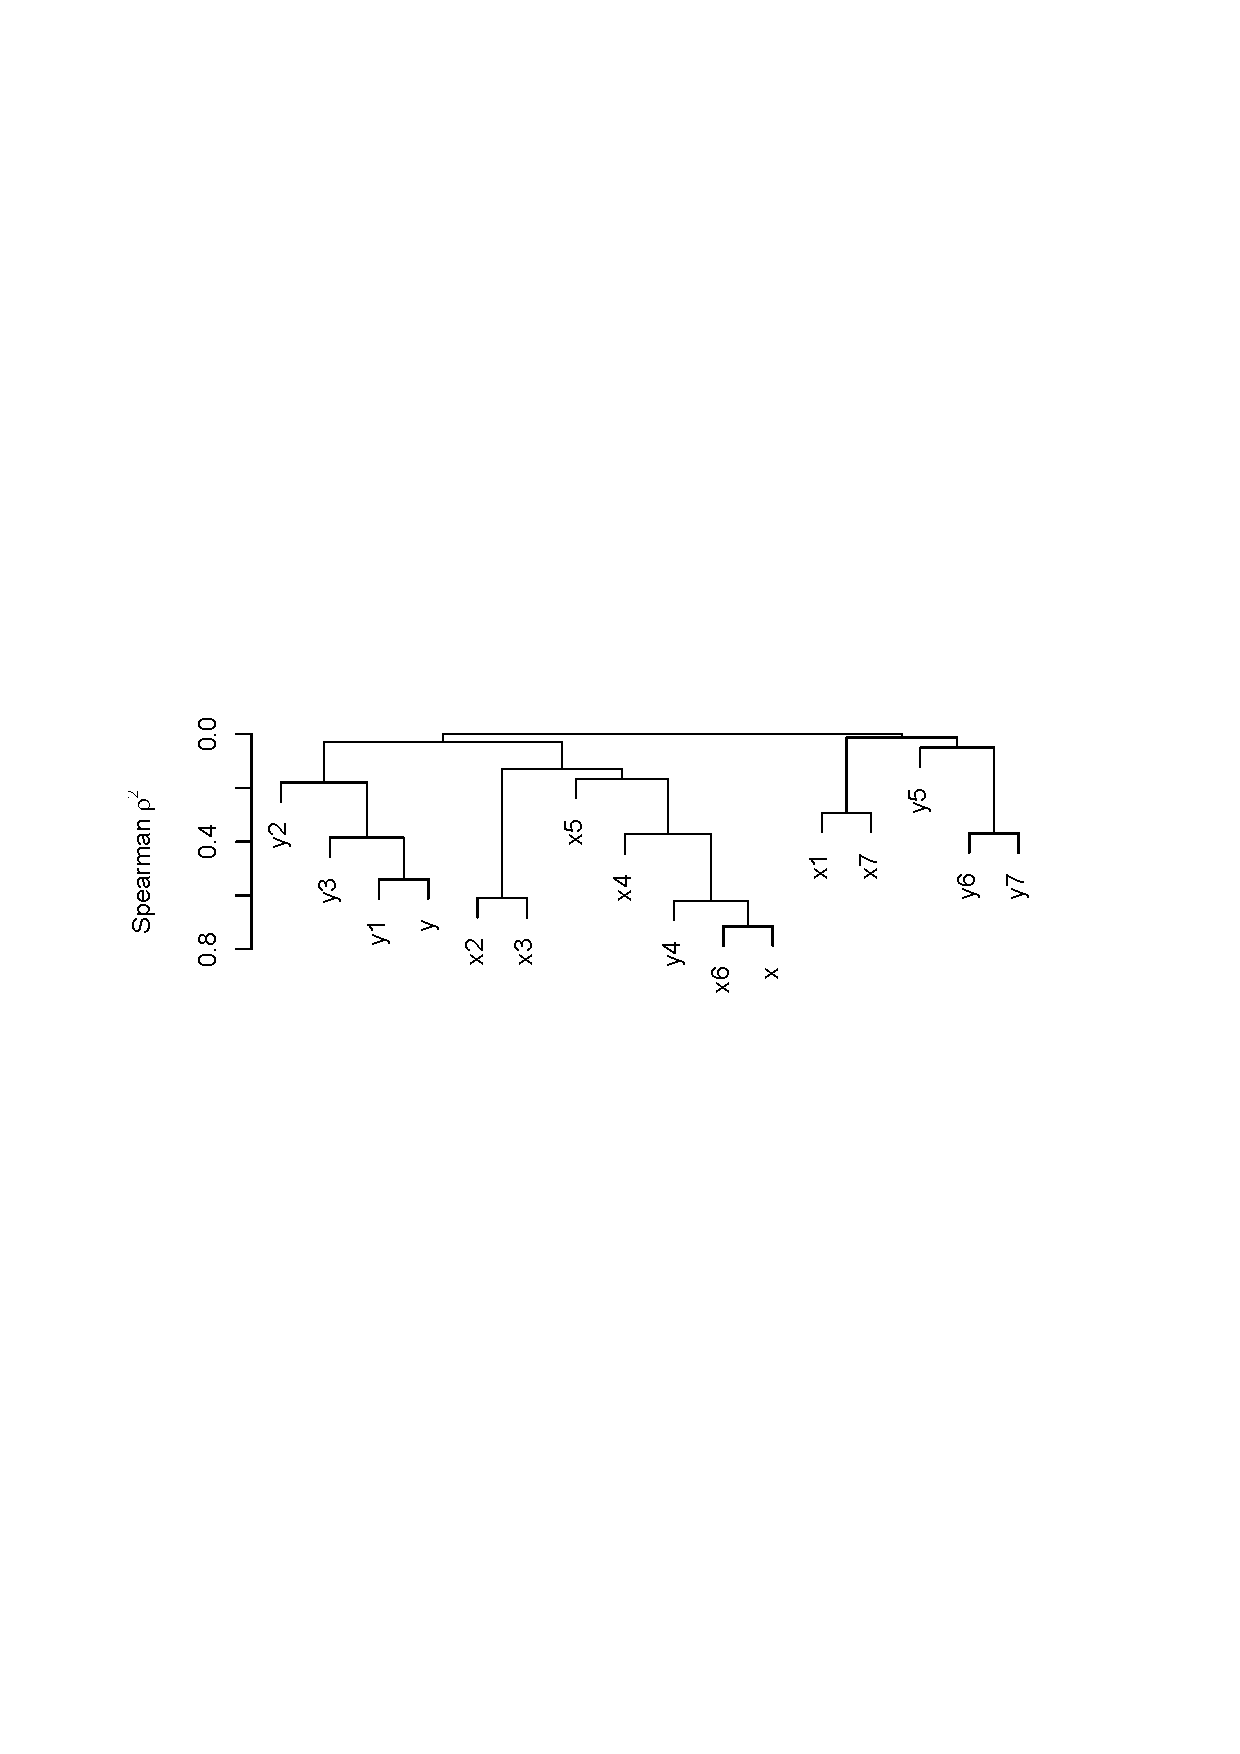
\includegraphics[width=\textwidth]{figures/14/fig4}
\begin{flushleft}
  \small Legend: x total formalization value, x1 inventory size, x2 host number (targets within NP), x3 locus operandi (targets outside of the NP), x4 obligatoriness, x5 boundedness, x6 multiple marking on various types of targets in the NP, x7 exhaustivity of classification, y total transparency value, y1 degree of semantic assignment, y2 number of different assignment rule types, y3 number of assignment rules, y4 \textsc{independence from other grammatical categories}, y5 discreteness of markers, y6 redundancy, y7 flexibility
\end{flushleft}%
\label{fig:WDG:4}
\end{figure}

\figref{fig:WDG:4} suggests that there are actually more than two dimensions and that the total indexes do not reflect all of their components equally well. The three first transparency features (y1--3), and apparently also the whole y-index, measure similar things, viz.\ how transparent assignment is, ranging from semantic to opaque. Degree of formalization (x) seems indeed to be an important issue, but, as it turns out, y4 (in)dependence of other grammatical categories \textendash{} even though arguably indicating transparency \textendash{} actually correlates with multiple marking on various types of targets in the NP (x6), obligatoriness (x4), and boundedness (x5), which seems to indicate that it is a characteristic property of a grammaticalized category of gender to exhibit interdependence with other grammatical categories.

We do not want to suggest here that gender does not exist if it does not cumulate with number, case, or person. However, where there is gender and no cumulation, gender tends to have a low degree of formalization. Notably, gender has a tendency not to be obligatory and not to be marked on multiple agreement targets, if it does not cumulate with other categories. Let us consider a few cases in point.

Within \ili{Sino-Tibetan}, \ili{Limbu} (\citealt[21]{Driem1987}) and other \ili{Kiranti} languages (\citealt[508]{Ebert2003a}) have a very limited masculine-feminine gender opposition on attributive adjectives (one target type). The suffixes, masculine  \textit{-pa/ba} and feminine \textit{-ma}, although they can be shown to be of nominal origin (\textit{ma} and \textit{pa} also mean `mother' and `father', for instance, in \ili{Camling}; \citealt[535]{Ebert2003b}), are common derivational suffixes in adjectives throughout \ili{Tibeto-Burman} languages. In \ili{Classical Tibetan} (\ili{Sino-Tibetan}, Bodish), adjectives have nominal suffixes (\mbox{\textit{-pa/}}\mbox{\textit{-ma/}}\mbox{\textit{-po/}}\mbox{\textit{-mo}} or \textit{-ka}): \textit{chen-po} `large', \textit{legs-pa} `good', \textit{gsha-ma} `worthy'; ``a few adjectives may express the natural gender of their referent by alternating the masculine \textit{pa/po} and feminine \textit{ma/mo} suffixes, but most adjective forms are fixed'' (\citealt[373]{DeLancey2003}). Not all adjectives, where the markers occur, do agree and agreement is not obligatory even in those adjectives where it occurs.

The \ili{Hindu Kush Indo-Aryan} languages \ili{Khowar}, \ili{Kalasha}, and \ili{Dameli} (\citealtvo{Liljegrenthisyear}) distinguish animacy in the root of the copula. Number and person are marked through suffixes attached to the animate/inanimate roots, and thus do not cumulate with the morpheme where animacy is marked.

Mopán Maya\il{Maya, Mopán} masculine and feminine gender (originating from person name markers) have only a single marking target. Only a minority of nouns are gendered and the gender marker can sometimes be omitted (\citealt[133]{Contini-Morava2018}).

In \ili{Ngan\textquotesingle{}gityemerri} (discussed in \sectref{sec:WDG:4.3}, included in Passer's sample), gender does not cumulate and not all nouns are classified in noun classes.

In languages where gender has been borrowed, gender is often not in cumulation with another grammatical category and not obligatory. For instance, \ili{Chamorro} has borrowed the \ili{Spanish} masculine and feminine gender markers as \textit{-o/u} and \textit{-a} along with \ili{Spanish} words which results in a semi-productive sex-based type of gender system without cumulative exponence (\citealt{Stolz2012}; \citealtv{DiGarbothisyear}).

However, before hasting to conclusions, it is important to note that degree of formalization has played an important role in delimiting gender from classifiers. Notably, obligatoriness is a traditional feature used for distinguishing between classifiers and gender (e.g., \citealt[160]{Dixon1982}: ``a grouping of all the nouns of a language [...] so that there is some overt indication of the class of a noun within any sentence in which it occurs''). According to these criteria, most of the languages discussed in this section would count as lacking gender. By applying these criteria, there is thus a danger of excluding by definition languages where gender has limited degree of formalization (see also \citealtv{Waelchlithisyear}). Yet, we have chosen to make the connection between gender and cumulation explicit in our definition of gender, which contains the statement that gender typically exhibits cumulative exponence with number, case, and/or person (see \sectref{sec:WDG:1}). However, this does not mean that categories lacking cumulation with other categories should be excluded from the study of grammatical gender.

  \subsection{Summary}

To sum up, cumulation of gender with number, case and/or person is pervasive across the languages of the world. In addition, in a few cases we are able to establish through diachronic comparison that cumulative exponence with other morphosyntactic features can be reconstructed, and thus exists from the very origin of the history of a language- and/or family-specific gender system. This can most likely be explained with the fact that gender tends to develop from pre-existing grammatical systems. For instance, gender may arise as a condition on the distribution of a specific number value (as in animacy-constrained plural marking) or case distinction (as in differential argument marking). More research is needed to explore the diachronic relationship between gender and number, case, and/or person, but it is fair to say that interdependence of gender with these other grammatical category types is the rule rather than the exception. This typological finding is in need of diachronic explanation in each individual instance.

Cumulative exponence is a violation of the Principle of One-Meaning--One-Form (one and the same affix is associated with two or more grammatical meanings) and the Principle of Independence (the encoding of gender distinctions is dependent on number, case, and/or person values) and thus qualifies as a phenomenon that fosters complexity (see \sectref{sec:WDG:2}). The fact that gender typically has cumulation with other nominal morphosyntactic features naturally means that gender is usually complex.

\section{Lexical plurality and grammatical gender}\label{sec:WDG:9}

\subsection{Introduction}\label{sec:WDG:9.1}
In many languages, certain nouns tend to be inherently specified for number, that is, to display lexicalized number values. This fact has been claimed to blur the boundaries between the gender and number domain. The gender systems of the Papuan languages \ili{Coastal Marind} and \ili{Walman}, described by \citetvo{Olssonthisyear} and \citetvo{Dryerthisyear} are a case in point, which we discuss in this section in the light of the larger typological context.

The label pluralia tantum is typically used in the literature to refer to nouns that only exist in the plural-marked form, as in \ili{English} \textit{scissors}, \textit{trousers}, \textit{leftovers}, and \textit{supplies}.%
\footnote{%
For a recent, typologically informed, classification of types of pluralia tantum nouns, see \cite{Corbett2018}.
} %
Broadly speaking, pluralia tantum nouns fall within the wider domain of \spterm{lexical plurality}. The term encompasses a variety of semantic and formal phenomena, both morphological and syntactic, which stem from the fact that plurality is a lexicalized property of a given noun, or, simply put, part of what there is to know about it (\citealt[2]{Acquaviva2008}). In this section we use the labels \spterm{lexical plurals} and \spterm{lexical plural nouns} as general terms to refer both to pluralia tantum nouns, that is, nouns with fixed plural number, as well as to nouns that are inherently plural, but that are not necessarily marked as plural.

Previous studies both on the spoken and signed modality (\citealt{Koptjevskaja-Tamm2001}; \citealt{Meer2015}; \citealt{Boerstell2017}) show that some broader semantic domains may be identified as recurrent attractors of lexical plurality across languages, while languages differ considerably with respect to the specific concepts that tend to be associated with lexical plurality. In \tabref{tab:WDG:17} we list some major semantic domains \textendash{} they need not necessarily exclude each other \textendash{} that have been shown to be most typically associated with lexical plurality. We illustrate each semantic domain with one exemplar concept with an \ili{English} label. Notice that the concept chosen to exemplify a particular semantic domain need not to be a lexical plural of \ili{English}, which is indicated by small caps.

\begin{table}[h]
\caption{Semantic domains associated with nominal lexical plurality across languages\label{tab:WDG:17}}
\begin{tabularx}{\textwidth}{Q>{\scshape}l}
\lsptoprule
Semantic domain 	& \normalfont	Exemplar concept\\
\midrule
Abstract\footnote{Abstract nouns can be either count or non-count and it is reasonable to suspect that it is the latter type that is especially likely to be attracted by the lexical plurality domain. We are grateful to Östen Dahl for this suggestion.}	&	anger\\
Collectives 	&	cattle\\
Dual entities/Internally complex concept 	&	glasses \\
Disease 	&	measles\\
Festivities and time intervals 	&	season\\
Liquids and masses 	&	saliva\\
Locations 	&	woods\\
Situations/activities involving more than one participant 	&	fight\\
\lspbottomrule
\end{tabularx}
\end{table}


Concepts typically expressed by lexical plurals differ in whether they are countable or non-countable, a distinction that not necessarily neatly aligns with the domains in \tabref{tab:WDG:17}. Countable units may refer to what we may think of as singular entities. The \ili{English} nouns \textit{leftovers} and \textit{supplies} have a mass noun reading and it is not possible to talk about one item of them. Liquids and masses are usually non-countable, but also abstract concepts often belong to this category. Conversely, we can talk about \textit{a pair of scissors/trousers}, which, in this respect, behave as count nouns. Languages differ as to whether they use special constructions to count multiple instances of a particular entity denoted by countable lexical plural nouns (as in \ili{English} \textit{one pair of scissors/trousers}), a topic which is not further addressed here.

As mentioned above, in spoken languages, nouns that are lexically plural typically only occur in the plural form. A parallel situation is found in the signed modality where lexical plurality is associated with double-handed signs, what \cite{Boerstell2017} refer to as \spterm{articulatory plurality}. Similarly to the spoken modality, where pluralia tantum nouns are typically marked by regular, productive number morphology, double-handed articulation is used in \ili{sign languages} to mark non-lexical, compositional plurality with various types of signs (Carl Börstell, p.c.).

\subsection{Lexical plurality and grammatical gender: a crosslinguistic overview}\label{sec:WDG:9.2}

If a language has number agreement, lexical plural nouns typically trigger plural agreement, and the formal marking patterns are typically indistinguishable from those triggered by morphological plurals. While this would seem to be a rather unproblematic fact, it turns out that in languages with grammatical gender and large classes of lexical plural nouns, lexical plurality may come to interact so closely with the morphosyntactic encoding of gender that the two domains (gender and number) may appear to be merged into one. This is the situation that we encounter in two of the Papuan languages investigated in the first volume of this work, \ili{Coastal Marind} \citep{Olssonthisyear} and \ili{Walman} \citep{Dryerthisyear}. Let us briefly summarize the \ili{Coastal Marind} and \ili{Walman} situations (for more extensive analyses, we refer to the individual chapters).

There are four genders in \ili{Coastal Marind}: masculine, feminine, and two inanimate genders, which Olsson refers to as gender I, II, III, and IV. While gender I and II vary according to number (singular and plural), the two inanimate genders are number-invariant. In addition, the plural marker used for the two animate genders (I and II) and the marker of gender IV are the same, and this syncretism is systematic across all agreement targets, even through the patterns of suppletion that regulate argument indexing on verbs. While male humans are gender I and female humans gender II, there are no strong tendencies that help predict which inanimate nouns should be assigned to gender III and which other ones to gender IV. Nevertheless, some regularities can be detected. For instance, some of the semantic domains that are typically associated with lexical plurality tend to cluster in gender IV (e.g., internally complex objects, diseases, heterogeneous objects). This, together with the fact that the plural marker of the animate genders is systematically syncretic with the marker of gender IV, suggests that there might be an even tighter relationship between gender IV and nominal plurality. According to Olsson, this relationship can be understood in diachronic terms. He speculates that at least some of the gender IV nouns are the diachronic descendants of a large class of pluralia tantum nouns which, as such, used to trigger semantically motivated plural agreement, the same plural agreement pattern triggered by animate masculine and feminine nouns. Such an originally coherent class of pluralia tantum nouns later expanded ``resulting in a large, semantically heterogeneous residue gender, with a small core that still reflects the `plural semantics' of the original pluralia tantum grouping'' (\citealtvo{Olssonthisyear}, p.~219).


\newpage 
\ili{Walman} has two clear-cut gender values, masculine and feminine. In addition, together with the diminutive, \citetvo{Dryerthisyear} describes lexical plural nouns as a gender-like phenomenon. Lexical plurals in \ili{Walman} are not marked as plural, but can be described as syntactically pluralia tantum nouns because, independently of whether their denotational meaning is singular or plural, they always trigger plural agreement. Semantically, the range of meanings expressed by lexical plural nouns in \ili{Walman} strongly overlaps with the semantic groupings identified in the typological literature on the topic: objects consisting of multiple parts, dual entities (especially body parts coming in pairs), mass nouns. While there can be mismatches (not all mass nouns are, for instance, pluralia tantum), the semantic makeup of this class of nouns is highly consistent. According to Dryer, what could justify describing the \ili{Walman} pluralia tantum nouns as an independent gender value, alongside masculine and feminine, is the sheer number of lexemes in this class: 81 instances of lexical plurals are attested in Dryer's corpus, as opposed to 40 instances of masculine nouns.

Interactions between lexical plurality and grammatical gender similar to those attested in \ili{Coastal Marind} and \ili{Walman} are also found in other New Guinean languages. An interesting parallel to \ili{Coastal Marind} is, for instance, the \ili{Ok} language \ili{Mian}. In \ili{Mian}, along with the masculine and feminine genders there are two inanimate genders: neuter 1, which is sensitive to number distinctions, and neuter 2, which is number-invariant and whose marker is the same as the plural of neuter 1 (for a detailed description of the gender system of \ili{Mian}, see \cite{Fedden2011}. \citetvo{Olssonthisyear} notes that in \ili{Mian} the overlap between neuter 2 nouns and the semantic domains typically associated with lexical plurality is even stronger than in \ili{Coastal Marind}.%
\footnote{%
Depending on the genealogical classification adopted, \ili{Anim} and \ili{Ok}, the language families to which \ili{Coastal Marind} and \ili{Mian}, respectively, belong, may be also seen as distantly related members of the Trans New Guinea phylum (see \sectref{sec:WDG:11.1}).
} %
In his survey of gender systems in the languages of New Guinea, \citetvo{Svaerdthisyear} mentions the case of another New Guinean language, \ili{Ama} (\ili{Left May}), where lexical plurals systematically align with one gender value in a way that is at least partially reminiscent of the \ili{Coastal Marind} system. There are three genders in \ili{Ama} \textendash{} masculine, feminine, compound \textendash{} and nouns that are semantically connected with lexical plurality (in particular, nouns denoting objects having many parts and mass nouns) are always assigned to the compound gender (\citealt[68]{Arsjoe1999}). In sum, the language-specific and cross-linguistic data presented in separate contributions to the two volumes of this work show that a number of genealogically unrelated New-Guinean languages have classes of nouns, which fall in between representing a proper gender value and an unusually large class of nouns with fixed plural number/lexicalized plurality. The spread of this pattern within New Guinea and its role as a possible characteristic feature of the gender systems of this area would deserve to be further investigated.

There are a few typological parallels to the New Guinean languages discussed above, where, other things being equal, lexical plurality has an impact on patterns of encoding in the domain of gender and number agreement. One such parallel is \ili{Cushitic} languages, or at least a subset of them. \ili{Cushitic} languages are a branch of the \ili{Afro-Asiatic} family, spreading from Eritrea all the way down to Tanzania and consisting of approximately 40 languages, further divided into four subgroups: \ili{Agaw}, \ili{Beja}, East \ili{Cushitic}, and South \ili{Cushitic}. Nominal number marking in \ili{Cushitic} is typically not obligatory. Speakers can leave nouns unmarked for number or use a variety of derivational suffixes and/or morphophonological strategies to mark a noun as singular or plural. In the literature on \ili{Cushitic} languages, number-unmarked nouns are referred to as nouns with general number or as transnumeral nouns, whereas the derivational singular and plural morphemes are labeled as singulative and plurative. \ili{Cushitic} languages typically have sex-based gender systems with a masculine-feminine distinction. Yet, some languages of the family are described as having three genders, with the third gender class beyond masculine and feminine being traditionally referred to as ``the plural''. There are two main scenarios under which some \ili{Cushitic} languages have been analyzed as displaying a tripartite gender system with a distinction between masculine, feminine and plural gender.

Under the first scenario, languages have agreement patterns that are used to signal that the controller is plural, but that are not used with all plural controllers. This is, for instance, the case of the East \ili{Cushitic} language \ili{Baiso}. The gender and number agreement system of \ili{Baiso} has been described in detail by \cite{Corbett1987} and \cite{Corbett2000}. In the following, we provide a brief overview of its most relevant properties.

\ili{Baiso} has two gender distinctions in the singular, masculine and feminine. Verbs agree in gender and number with the subject. With the majority of plural-marked nouns, the agreement pattern triggered by the verb is the same as the one triggered by masculine singular nouns, irrespective of whether the noun is masculine or feminine. This is illustrated in examples (\ref{ex:WDG:75}) and (\ref{ex:WDG:76}), which show gender and number agreement with masculine singular and plural nouns, and feminine singular and plural nouns, respectively.

\protectedex{%
\ea\label{ex:WDG:75}
\ili{Baiso} (\ili{Afro-Asiatic}, East \ili{Cushitic}; \citealt[181]{Corbett2000}): gender and number agreement with masculine nouns\\
\begin{xlist}
\ex
\gll	lúban 	hudure \\
lion(\textbf{\textsc{m}}).\textsc{general} 	slept.\textbf{\textsc{m}} \\
\glt	`The lion slept.' \\
\ex
\gll 	luban-\textbf{jool} 	hudure \\
	lion-\textbf{\textsc{pl}} 	slept.\textbf{\textsc{m}} \\
\glt	`The lions slept.' \\
\end{xlist}
\z
}%

\ea\label{ex:WDG:76}
\ili{Baiso} (\ili{Afro-Asiatic}, East \ili{Cushitic}; \citealt[182]{Corbett2000}): gender and number agreement with feminine nouns\\
\begin{xlist}
\ex
\gll 	kimbír 	hudurte \\
	bird(\textbf{\textsc{f}}).\textsc{general} 	slept.\textbf{\textsc{f}} \\
\glt	`The bird slept.' \\
\ex
\gll 	kimbir-\textbf{jool} 	hudure \\
	bird-\textbf{\textsc{pl}} 	slept.\textbf{\textsc{m}} \\
\glt	`The birds slept.' \\
\end{xlist}
\z

In addition to the two verb forms exemplified in (\ref{ex:WDG:75}) and (\ref{ex:WDG:76}), \ili{Baiso} has a third verb form, which is only used when the subject (i.e., the controller noun) is the third person plural pronoun, a noun marked by the paucal suffix or one of the underived nouns listed in \tabref{tab:WDG:18}. Because it is used with third person plural pronouns, this third verb form is traditionally glossed as \textsc{pl}, ``plural''. The use of the plural verb form with two paucal-marked nouns (one masculine and one feminine) is illustrated in (\ref{ex:WDG:77}).

\ea\label{ex:WDG:77}
\ili{Baiso} (\ili{Afro-Asiatic}, East \ili{Cushitic}; \citealt[181--182]{Corbett2000}): plural agreement\\
\begin{xlist}
\ex
\gll 	luban-\textbf{jaa} 	hudureene\\
lion-\textbf{\textsc{pauc}} 	slept.\textbf{\textsc{pl}} \\
\glt		`A few lions slept.' \\
\ex
\gll 	kimbir-\textbf{jaa} 	hudureene\\
bird-\textbf{\textsc{pauc}} 	slept.\textbf{\textsc{pl}} \\
\glt		`A few birds slept.' \\
\end{xlist}
\z

\begin{table}
\caption{Underived nouns selecting plural agreement in Baiso, adapted from \cite[9]{Corbett1987}\label{tab:WDG:18}}
\begin{tabularx}{\textwidth}{lX}
\lsptoprule
Semantic groupings 	&	Nouns 	\\
\midrule
Body parts 	&	\textit{ilkoo} `tooth, teeth'; \textit{kalaljaa} `kidneys'; \textit{luk̟k̟aa} `foot, feet, leg(s)'; \textit{ilo̟ o} `eye(s)'; \textit{ogorroo} `hair'; \textit{moo} `hips, lumber region' 	\\
Collectives 	&	\textit{saé} `cattle' 	\\
Mass nouns 	&	\textit{eenoo} `milk'; \textit{soo} `meat'; \textit{udú} `faeces' 	\\
Objects coming in pairs 	&	\textit{keferoo} `sandals' 	\\
\lspbottomrule
\end{tabularx}
\end{table}

The eleven nouns in Table 18 always select the plural verb form. The noun for `kidneys', \textit{kalaljaa}, can be described as a ``paucal tantum'' noun as it is only attested in the paucal-marked form (\citealt[9]{Corbett1987}). The suffix \textit{-oo}, in which many of the nouns listed in the table end, is a productive plural suffix in several \ili{Omo-Tana} languages, a subgroup within East \ili{Cushitic} to which \ili{Baiso} also belongs. However, \textit{-oo} is not a productive plural suffix in \ili{Baiso} (\citealt[19]{Corbett1987}). Within \ili{Cushitic} studies, the agreement pattern illustrated in (\ref{ex:WDG:77}) has been analyzed as the morphosyntactic realization of a third gender, the plural gender (\citealt[146]{Mous2008}). The analysis is motivated by the fact that the nouns listed in \tabref{tab:WDG:18} select plural agreement even though they are morphologically underived for number. For these nouns, plurality is a lexically specified feature as masculine and feminine are for other nouns. \cite{Corbett1987} and \cite{Corbett2012} describe the peculiar agreement preferences of the nouns listed in \tabref{tab:WDG:18} as lexical exceptions and reject the analysis of plural as a gender value. Semantically these nouns tend to denote collectives (`cattle'), entities that are prone to occur as pairs (`kidneys'), or masses (`meat'). They always select plural agreement because they are semantically and lexically plural. \cite[121--127]{DiGarbo2014} develops this line of reasoning one step further and describes \ili{Baiso} as a language with a split system of number agreement. While the majority of nouns that undergo regular morphological plural marking do not trigger dedicated plural agreement but an agreement pattern that is syncretic with the one triggered by masculine singular nouns, as in examples (\ref{ex:WDG:75}) and (\ref{ex:WDG:76}), dedicated plural agreement is used only with a closed set of controllers: plural pronouns, paucal-marked nouns, the lexical plurals and a handful of plural-marked nouns that tend to denote small groups. \cite{DiGarbo2014} speculates that the split number agreement system attested in \ili{Baiso} is semantically motivated and that the controllers of dedicated plural agreement rank higher on a scale of semantic plurality than derived plural nouns.

There is yet another profile of languages within \ili{Cushitic} that has been analyzed as displaying a tripartite gender system with plural as a gender value along with masculine and feminine. These are languages that have dedicated patterns of plural agreement that are used with all plural controllers: third person plural pronouns, derived plurals (that is, nouns that are morphologically marked as plural), and nouns that are unmarked for number but nevertheless control plural agreement. In these languages, gender distinctions are always neutralized in the plural. In addition, in these languages nouns that are number-unmarked but that always trigger plural agreement constitute a rather large lexical class. This large class of inherently plural nouns encompasses both typically lexical plural concepts and concepts that are not associated with lexical plurality, somewhat similarly to nouns of gender IV in \ili{Coastal Marind}. An example of such a language is \ili{Konso}, an East \ili{Cushitic} language spoken in Ethiopia. \ili{Konso} displays subject agreement on the verb, which has three different inflectional forms depending on whether the subject argument is masculine (\ref{ex:WDG:78}a), feminine (\ref{ex:WDG:78}b) or plural (\ref{ex:WDG:78}c and d). The masculine and feminine forms are used if the subject is singular, the plural form is used if the subject is a plural-marked noun (\ref{ex:WDG:78}c) or a noun that is lexically specified as plural (\ref{ex:WDG:78}d). Definite markers, which are suffixed to nouns, only distinguish between singular and plural. The plural form of the definite marker is used both with overtly plural-marked nouns and with nouns that are lexically specified as plural.

\ea\label{ex:WDG:78}
\ili{Konso} (\ili{Afro-Asiatic}, East \ili{Cushitic}; adapted from \citealt[36--37]{Tsegaye2017}): gender and number agreement\\
\begin{xlist}
\ex
\gll 	ʛmayta-\textbf{siʔ} 	i=kutiʔ-\textbf{ay}\\
old.man-\textbf{\textsc{def.sg}} 	3=sit.down-\textbf{\textsc{pfv.3m}} \\
\glt	`The old man sat down.' \\
\ex
\gll	aleeta-\textbf{siʔ} 	i=piʔ-\textbf{t}-i \\
hut-\textbf{\textsc{def.sg}}	3=fall-\textsc{\textbf{3f}-pfv} \\
\glt	`The hut fell.' \\
\ex
\gll 	laha-ɗɗ-\textbf{siniʔ} 	i=muk-i-\textbf{n} \\
ram-\textsc{pl-\textbf{def.pl}} 	3=sell-pass-\textsc{ipfv.fut-\textbf{3pl}} \\
\glt	`The rams will be sold.' \\
\ex
\gll	filaa-\textbf{siniʔ} 	i=pat-i-\textbf{n}\\
comb-\textbf{\textsc{def.pl}} 	3=be.broken-\textsc{pfv-\textbf{pl}} \\
\glt	`The comb disappeared.' \\
\end{xlist}
\z

\cite{Orkaydo2013} and \cite{Tsegaye2017} analyze the plural agreement pattern, as realized on verbs and definite markers, as the morphosyntactic manifestation of a gender value. According to this analysis, plural-marked nouns are also considered to be plural in gender. The main arguments that \cite{Orkaydo2013} and \cite{Tsegaye2017} present in support of the plural as a gender-value analysis in \ili{Konso} are: (i) the large number of nouns that are underived for number and only trigger plural agreement%
\footnote{%
\cite[318--330]{Orkaydo2013} lists 471 \ili{Konso} nouns. Out of these, 92 are classified as being inherently plural (or, following his analysis, plural in gender), 134 as feminine, and 245 as masculine.%
} %
and (ii) the fact that not all of these nouns are semantically analyzable as instances of lexical plurals.%
\footnote{%
By inspecting the meanings of the 92 nouns classified by \cite[318--330]{Orkaydo2013} as inherently plural we found that more than half of them (about 50) have denotational meanings that align with the most typical semantic domains of lexical plurality (e.g., mass nouns, body parts coming in pairs, names of activities requiring multiple participants).
}%

The possibility of positing an independent gender value for lexical plural\slash pluralia tantum nouns has also been defended for \ili{Russian} by \cite{Zaliznjak1977}. \ili{Russian} has a tripartite gender system with a masculine-feminine-neuter distinction that is further subject to a number of animacy-based conditions. Gender distinctions are neutralized in the plural. Pluralia tantum nouns always trigger plural agreement, irrespectively of whether they refer to singular or plural entities. This is illustrated in (\ref{ex:WDG:79}).

\ea\label{ex:WDG:79}
\ili{Russian} (\ili{Indo-European}, \ili{Slavic}; \citealt[237]{Corbett2012}) \\
\gll odn-\textbf{i} 	san-\textbf{i}\\
one-\textbf{\textsc{pl.nom}} 	sledge-\textbf{\textsc{pl.nom}} \\
\glt `one sledge' \\
\z

\noindent In virtue of the properties illustrated in (\ref{ex:WDG:79}), according to Zaliznjak, pluralia tantum nouns in \ili{Russian} are better analyzed as representing one independent agreement class, and thus one independent gender value.

\cite[237--238]{Corbett2012} notices that \emph{plural-as-a-gender-value} analyses have only been proposed for languages where gender distinctions are systematically neutralized in the plural. This is the case for \ili{Russian} and indeed this is also the case for \ili{Coastal Marind}, \ili{Walman}, \ili{Baiso} and \ili{Konso}. In languages where gender distinctions are maintained in the plural, lexical plurals are usually distributed across different gender values, but still share the properties of carrying only plural morphology and/or of only triggering plural agreement. This is for instance the case of \ili{Italian}, where the plurale tantum noun \textit{pantaloni} `trousers' is masculine and selects only masculine plural agreement while the plurale tantum \textit{forbici} `scissors' is feminine and selects only feminine plural agreement as in \textit{i pantaloni} `the.\textsc{f.pl} trousers' and \textit{le forbici} `the.\textsc{m.pl} scissors'. Analyzing \ili{Italian} pluralia tantum nouns as belonging to separate gender values would then mean positing at least two different lexical plural genders in the language, one formally overlapping with the masculine plural and one with the feminine plural. \cite[237--238]{Corbett2012} uses this argument to reject the cross-linguistic validity of \textit{plural-as-a-gender-value} analyses. Conversely, he stresses that in languages where gender distinctions are neutralized in the plural, lexical plural nouns are de facto outside the system of gender distinctions because this system is only active in the context of singular number, which they are devoid of. The exceptional agreement preferences of these nouns are thus to be analyzed as a consequence of them being irregular from the point of view of number and not of gender.

While we agree that having or not having gender distinctions in the plural is a relevant typological parameter to take into account when assessing the type of encodings that lexical plurality may trigger in the domain of gender and number agreement, we believe that language-specific analyses where lexically plural nouns are described as making up a gender value of their own \emph{should not} be a priori considered to be fallacious. The descriptive adequacy of language-specific categories should always be distinguished from what is generalizable across languages with the support of typologically adequate comparative concepts (\citealt{Haspelmath2010}). Arguing, and demonstrating, that lexical plural nouns in some gendered languages exhibit gender-like properties does not amount to say that the lexical plural nouns of all languages with gender should be analyzed as instances of an independent gender value. In languages like \ili{Coastal Marind} and \ili{Konso}, the lexicalization of the plural number value and the presence of large classes of nouns with fixed plural number, which only trigger plural agreement, clearly blurs the distinction between the gender and number domain.


  \subsection{Extreme lexicalization of number values in Kiowa-Tanoan}
\largerpage[1.5]
In addition to the cases mentioned in \sectref{sec:WDG:9.2}, the gender system of yet other languages may be described as being entirely based on the lexicalization of number values.\footnote{%
This subsection was written by Bruno Olsson. We are very thankful to Bruno for his general contribution to our discussion of gender and lexical plurality.}
\clearpage 

The most extreme cases of lexicalization of number values are arguably found in the languages of the \ili{Kiowa-Tanoan} family of North America, illustrated here with \ili{Kiowa} data from \cite[310]{Sutton2014} and \cite[78]{Watkins1984}. \ili{Kiowa} distinguishes singular, dual and plural numbers through a combination of suffixation on nouns and indexing prefixes on verbs. Nouns occur in two forms: the unmarked basic form and the inverse form, derived by suffixation. For every noun in the language it must be specified whether the noun occurs in the basic or the inverse form when reference is made to one, two or three or more entities (the labels basic and inverse are specific to the \ili{Kiowa}-Tanoan descriptive tradition and should not be confused with similar labels in other grammatical traditions). For example, \textit{tógúl} `young man' is used in the basic form for reference to one or two young men, whereas the inverse form \textit{tógúˑdɔ́} must be used for reference to three or more young men. This contrasts with the noun \textit{ˀɔnsóˑ} `feet', which occurs in its basic form when reference is made to two or more feet, but in the inverse form \textit{ˀɔnsôy} when reference is made to a single foot. For other nouns the basic form refers to two instances of the referent, as with \textit{ˀálɔˑ} `(pair of) apples', whose inverse form \textit{ˀálɔˑbɔ} is used to refer to one apple or three or more apples. A fourth type of nouns lacks the inverse form and occurs in the basic form regardless of the cardinality of the referents.

Each noun in the language exhibits the basic-inverse alternation according to one of these four patterns. In the \ili{Kiowa-Tanoan} literature the four patterns are referred to as noun classes and numbered I-IV (following \citealt{Wonderly1954}). Nouns in the four superclasses are further divided into subclasses according to their combinatorics with verb prefixes indexing person/number of core arguments. The intransitive third person paradigm consists of four prefixes: singular Ø-, dual \textit{ę̀-}, plural \textit{gyà-} and inverse \textit{è-}. The inverse verb prefix occurs whenever the inverse form of the noun is used, and the singular and dual disambiguate the number reference of nouns in their basic form. It is the behavior of the plural prefix that reveals the need for subclasses. For example, some class II nouns (`bucket', `saw', `arrow') trigger the plural prefix when reference is made to three or more entities, while other class II nouns (`bed sheet', `peg, stake', `peyote, cactus') trigger the singular prefix when reference is made to three or more entities; these two patterns form subclasses IIa and IIb. When the full range of indexing patterns is taken into account, the total number of subclasses is between 7 (e.g. \citealt{Watkins1984}) and 9 (\citealt{Harbour2008}; the difference in granularity depends on whether some marginal patterns are counted as their own subclasses or not).

\largerpage
It is clear from Wonderly et~al.'s (\citealt*{Wonderly1954}) use of the term \textit{noun classes} that researchers realized early on that the \ili{Kiowa-Tanoan} system of number marking amounts to a form of noun classification. Nichols' (\citeyear[141]{Nichols1992}) conclusion that ``noun classification appears to have arisen out of number agreement in the \ili{Kiowa-Tanoan} family'' explicitly couches this in diachronic terms (an interpretation repeated by \citealt[377]{Aikhenvald2000} and \citealt[451]{Luraghi2011}).

The parallel with languages such as \ili{Coastal Marind}, \ili{Walman}, \ili{Konso} and \ili{Baiso} is most evident in the class of \ili{Kiowa} nouns that trigger invariant plural prefixation on the verb regardless of the cardinality of the referent (class IVc in \citealt{Watkins1984}). According to \cite[46]{Harbour2008} this class consists of objects composed of several parts (`trousers', `book', `necklace', `tepee', `headdress'; the multi-part semantics are also noted by \citealt[270]{Merrifield1959}, ``a single item is looked upon as having several constituent parts''), granular mass nouns (`flour', `salt', `sand') and abstracts (`problem', `dance', `word, language'), which echoes the pluralia tantum-like semantics of the nouns discussed for \ili{Coastal Marind}, \ili{Walman}, \ili{Konso} and \ili{Baiso}. The important difference is that \ili{Kiowa} takes the lexicalization much further, and requires that every noun in the language be specified for its ``inherent number''. For some of the \ili{Kiowa} noun classes this can be expressed straightforwardly as an inherent number value, so that \ili{Kiowa} \textit{kʰɔ́ˑdé} `trousers' (class IVc) is inherently plural, and \textit{ˀálɔˑ} `(pair of) apples' (class III) is inherently dual. For other classes the pattern is more complicated, as with \textit{tól} `peg, stake' (class IIb) which triggers singular verb prefix when the cardinality of the referent is 1, the dual prefix with cardinality 2, but the singular also when cardinality is 3 and higher.

We think that the \ili{Kiowa-Tanoan} systems of ``inherent number'' must be considered gender according to the Hockettian conception of gender as ``classes of nouns reflected in the behavior of associated words''. This also seems to be the contention of Harbour, who \textendash{} working in the Chomskyan tradition \textendash{} equates the \ili{Kiowa} noun classes with \ili{Indo-European} gender, with the main difference residing in their semantic basis: the former is based on number and the latter on sex. For our purposes, the important point is that \ili{Kiowa-Tanoan} languages represent the extreme end of a spectrum in which the organization of nominal number in a language can be more or less gender-like. Further towards the other end of the spectrum we find languages such as \ili{Coastal Marind}, \ili{Walman}, \ili{Konso} and \ili{Baiso}, in which lexicalized number (in this case, plurality) appears to have blurred the line between gender and number to a much lesser degree.

  \subsection{Summary}
We believe that a particularly promising direction of research on the interaction between gender and lexical plurality lies in diachrony and, in particular, in examining how the encoding of lexical plurality affects the evolution of gender and number agreement systems. \citetvo{Olssonthisyear} suggests that a plausible explanation for the peculiar configuration of gender IV in \ili{Coastal Marind} is that this agreement class evolved from a smaller nucleus of pluralia tantum nouns (which selected plural agreement because semantically plural) and only gradually came to include non-plural types of nouns. A similar hypothesis could be tested on \ili{Konso} and other \ili{Cushitic} languages exhibiting large classes of lexical plural nouns. Another promising area of investigation in this domain would be taking a closer look at languages like \ili{Baiso}, where only certain types of agreement controllers, among which the lexical plurals, trigger the use of dedicated plural agreement, whereas the majority of morphologically plural nouns trigger agreement patterns that are syncretic with either masculine or feminine singular agreement. These languages, where, synchronically, there seems to be a split in the agreement patterns associated with nominal plurality, offer an interesting test case for hypotheses about the evolution and grammaticalization of number agreement, a topic that goes beyond the scope of the present volume.


\section{System evolution}
\label{sec:WDG:10}

  \subsection{Introduction}

\textit{System} is probably the most commonly unexplained term in the literature on grammatical gender and thus arguably rather void of meaning. However, in this section, we will argue that the notion of system is highly important from a developmental point of view. Furthermore, the relationship between complexity and system needs to be sorted out. The \ili{Latin} adjective \textit{complex} `weaved together' and the \ili{Ancient Greek} noun \textit{sústēma} `(what is) standing together' are very close in their original meanings. It is thus not surprising that complexity is often understood in linguistics as system complexity, which somehow wrongly takes for granted that complexity is necessarily connected to systems, especially if complexity is understood in terms of description length.

A very simple way of defining system in linguistics is to say that it is an opposition of at least two markers, and in this sense gender is always organized in terms of systems. However, this simple definition does not capture many of the systematic properties of mature gender. Gender connects different parts of language structure (one might say that it is always a multiple-interface phenomenon): syntax, semantics, and morphology are always involved. Lexicon is fundamentally involved to the extent that gender is lexical. Even phonology is sometimes involved, notably if there is phonological gender assignment. Mature gender systems imply a high degree of internal organization and, from a developmental perspective, it is interesting to consider how such complex systems can emerge.

In \sectref{sec:WDG:10.2} we introduce the notion of co-evolution (a set of more than one diachronic change, which are at least partly dependent on each other), which is crucial for processes of system emergence. In \sectref{sec:WDG:10.3} we discuss various approaches dealing with contextualization of variability where variation that is not accounted for is remotivated. In \sectref{sec:WDG:10.4} we will argue that co-evolution in both rise and reduction of gender can take the form of cascades of anomalies.

  \subsection{Co-evolution}
  \label{sec:WDG:10.2}

Diachronic processes, such as sound change, analogy, reanalysis, grammaticalization, and semantic shift, are often viewed as individual changes. One sound, morpheme, construction or meaning turns into another sound, morpheme, construction or meaning. However, changes can also co-occur in a sequence of connected events. The probably best-known example are push and drag chains of several sound changes that co-determine each other, such as the great vowel shift in \ili{English}. Since gender consists of systems of at least two markers, individual diachronic processes are usually not sufficient for the modelling of the emergence and evolution of gender. Of course, it cannot be excluded that several changes that may result in a gender system co-occur accidentally, but more often than not there will be some sort of co-evolution of several changes in the evolution of gender.

Even a maximally simple gender system, such as the \ili{Japanese} (Japonic) grammatical anaphors, \textit{kanojo} `she' (from the attributive form of the obsolete distal demonstrative in its attributive form \textit{kano} plus the Sino-\ili{Japanese} form \textit{jo} for `woman') and \textit{kare} `he' (from the independent form of the obsolete distal demonstrative; see \citealt{Ishiyama2008} and \citealtv{Waelchlithisyear}), is difficult to imagine without some sort of co-evolution. It is true that the loss of the distal demonstrative series \textit{kano/kare} is a shared development that is important for rendering both forms opaque, but the forms are still heterogeneous. One is a complex NP, the other one is just a simplex demonstrative form. The development of \textit{kare} to masculine `he' presupposes a semantic shift of narrowing to masculine, and this process is hard to imagine without co-evolution of a parallel feminine form that makes that narrowing possible.

It is thus not surprising that the general literature on grammaticalization, which focuses on individual cases of grammaticalization, says very little about the origin of gender. \cite{Heine2002} only list a few cases such as \textsc{man} (`man', `male', `person') > \textsc{third person pronoun} in \ili{ǁAni} (\ili{Khoe}-Kwadi, \ili{Khoe}), \ili{Lendu} (Central \ili{Sudanic}, Lenduic), and \ili{Zande}.


  \subsection{Contextualization of variability}
  \label{sec:WDG:10.3}

In a system, there are markers and a division of labor among them. It is a reasonable assumption that the markers (often of rather heterogeneous origin) are there first and that the division of labor is put into place in a second step. Here we will discuss two approaches that can help us understand how this can happen: Lass' (\citealt*{Lass1990}) concept of exaptation and the experimental research on iterated artificial language learning by Kirby and Smith and collaborators (\citealt{Kirby2008}; \citealt{Smith2010}).

\cite{Lass1990} borrows the term \spterm{exaptation} from biology where it means the ``opportunistic co-optation of a feature whose origin is unrelated or only marginally related to its later use'' (\citealt[80]{Lass1990}), such as when the dinosaur ancestors of birds happen to have feathers which later turn out to be useful for flying. Linguistic exaptation is the development by which junk that is kept (instead of being relegated) is later used for some other purpose. \cite{Lass1990} discusses the following two examples. (i) \ili{Indo-European} distinguished perfect and aorist in the past, a distinction which was lost in \ili{Germanic}, where the perfect and aorist stem forms were redeployed as singular and plural past stems in strong verbs. (ii) The \ili{Dutch} alternation between suffix \textit{-e} and Zero in attributive adjectives expressing gender and number agreement was redeployed in \ili{Afrikaans} as an expression of various classes of adjectives (among other things, simple versus complex/compound adjectives).

\cite{Smith2010} use iterated learning modelled in an experiment as a tool for investigating the cultural evolution of language. One group of participants is presented with some stimuli they have to learn and the next group of participants has to learn the language reproduced by the first group and so on in several ``generations''. The equivalent of Lass' ``junk'' is free variation in the input. In Smith \& Wonnacott's (\citealt*{Smith2010}) experiment, learners were presented with nouns denoting animals with the two artificial plural words \textit{fip} and \textit{tay} distributed entirely randomly in the input for the first ``generation''. This junk, or pattern of free variation between two plural marking strategies, was redeployed in iterative learning. Smith \& Wonnacott's (\citealt*{Smith2010}) call this \spterm{probability-matching behavior}: the learners reproduce markers more or less with the same proportion of frequency that the markers have in the input. However, as a consequence of transmission over several generations, the distribution of markers is made predictable by linking it to particular conditions, in this case the use of markers is made predictable by lexical conditioning. ``A typical fifth-participant language exhibits [...] predictable variability [...] for instance, \textit{fip} used to mark plurality on \textit{cow} and \textit{pig}, \textit{tay} used to mark plurality on \textit{rabbit} and \textit{giraffe}'' (\citealt[447]{Smith2010}). The learners thus developed some sort of lexical gender. While the token frequency of markers changes very little, there is a change from zero predictability to full or almost full predictability. As a consequence, conditional entropy drops, and if entropy is considered a measure of complexity, complexity drops. (Even though system complexity increases as we go from one grammatical distinction, number, to two, number and gender).

Lass' and Smith \& Wonnacott's examples have in common that there is a co-evolution of many changes. Parallel changes take place in all \ili{Germanic} strong verbs, all \ili{Afrikaans} attributive adjectives and all nouns denoting animals in the experiment. Unmotivated alternations are conditioned, which makes the alternation predictable (lower complexity as meaning and form are better aligned) at the cost of a lower independence (higher complexity according to the Principle of Independence), while the number of markers remains constant.

In \sectref{sec:WDG:7.5} and \sectref{sec:WDG:8} we have seen that gender may emerge as a condition on an already existing grammatical category. This may seem strange if viewed as a complexification in terms of the Principle of Indepencence without any obvious benefit since grammatical gender does not seem to provide any communicative benefit. However, rise of gender is better understandable if we assume that the stage before there was gender contained some markers whose use was largely unpredictable. In more general terms, we can assume that the stages that precede the development of gender contain anomalies where some formal distinctions are poorly motivated. This can, for instance, be due to sound change, to decategorialization of nouns, or to anaphoric NPs having become opaque (as in \ili{Japanese}).

  \subsection{Reduction and rise of gender as cascades of anomalies}
  \label{sec:WDG:10.4}

Gender system evolution often involves a sequence of changes where the first change introduces increasing complexity in the form of unpredictable variability and subsequent changes restore order. Such an initial change introducing idiosyncratic patterning can be regular sound change. A well-studied example is the loss of gender agreement in the predicative adjective (but not in the attributive adjective) in \ili{German} (\citealt{Fleischer2007a}, \citealt{Fleischer2007b} and the literature surveyed there). Old High \ili{German} and \ili{Old Saxon} had two competing inflectional paradigms of adjectives, one with endings originating from the pronominal paradigm and one with nominal endings. The nominal endings happened to be reduced to zero by regular sound change in all three genders in the nominative singular and in the nominative neuter plural. The idiosyncratic distribution created by phonological erosion is reflected quite accurately in \ili{Old Saxon} in predicative use (\textsc{sg} 0\%, \textsc{m.pl} 99\%, \textsc{f.pl} 95\%, \textsc{n.pl} 29\%; \citealt[Table~9]{Fleischer2007a}). In Early \ili{Old High German}, two opposite tendencies can be observed in predicative use. On the one hand, inflection tends to be lost in the forms where it was preserved. On the other hand, inflection is also partly reintroduced by analogy to the forms where it was not lost by sound law. Inflected forms spread most easily to the neuter plural and to a lesser extent also to the feminine singular, which happened to have the same pronominal ending as the neuter plural (\textsc{n.sg} 0\%, \textsc{m.sg} 1\%, \textsc{f.sg} 8\%, \textsc{n.pl} 64\%, \textsc{f.pl} 79\%, \textsc{m.pl} 80\%; \citealt[Table~11]{Fleischer2007a}). While the uninflected forms were generalized in predicative use in Middle High \ili{German} and Modern \ili{German}, the inflected forms were generalized in Highest \ili{Alemannic} dialects with support of language contacts with \ili{Romance} languages (\citealt{Fleischer2007b}). In attributive use, the inflected pronominal forms with gender and number agreement were generalized in all varieties of \ili{German}.

In the development simulated by \cite{Polinsky2003} for the transition from \ili{Latin} to Old \ili{French}, ``the major push for the restructuring of the gender system came from phonological changes (loss of vowel length, loss of word-final segments)'' (\citealt[385]{Polinsky2003}). Neuter merged with masculine in the singular and with feminine in the plural (as preserved in \ili{Romanian}). In early Old \ili{French} text, \ili{Romanian}-like neuter nouns had been reduced to about 4.6\% as compared to 21.1\% neuter in Classical \ili{Latin}.

There are also cascades of changes where an anomaly is remedied by restructuring which entails another anomaly which again calls for restructuring which in its turn is an anomaly and so on. Such a cascade of changes is responsible for a strange pattern in some Tamian \ili{Latvian} dialects in northern Kurzeme where demonstratives do not agree in gender anymore (only in number and case) and always take the masculine form (\ref{ex:WDG:80}).
\largerpage

% \protectedex{%
\ea\label{ex:WDG:80}
Kandava Latvian\il{Latvian, Kandava} (\ili{Indo-European}, \ili{Baltic}; \citealt{Graudina1958}; \citealt[65]{Rudzite1964}; \citealt[144]{Waelchli2018})\\
\gll un	tas	cũkgans	a	\uline{visàm}	\textbf{tiẽm}	\uline{cũkam}	tur	i	palic:s.\\
and	that.\textsc{nom.sg.m}	swineherd\textsc{(m).nom.sg}	with	all.\textsc{dat.pl.\uline{f}}	that.\textsc{dat.pl.\textbf{m}}	swine\textsc{(\uline{f}).dat.pl} there	be.\textsc{prs}.3	stay.\textsc{pst.ptcp.act.nom.sg.m}\\
\glt `and this swineherd had remained there with all those pigs'\\
\z
% } %

The starting point is a regular sound change (triggered by language contact with the \ili{Finnic} contact language \ili{Livonian}) where short vowels in final syllables of words longer than one syllable are lost. This causes gender neutralization (of masculine and feminine) in the accusative plural in nouns. Demonstratives are monosyllables and monosyllables are not affected by the sound change entailing neutralization. However, the neutralization is extended to them by analogy. The masculine accusative plural form in demonstratives is generalized also with feminine controllers. Since there is a syncretism of feminine plural accusative and nominative, the use of masculine forms instead of feminine is extended also to the nominative plural, which causes the gender opposition in the demonstrative plural forms to be maintained only in the dative (attested in the dialect of Zlēkas). This is a new anomaly, the dative is less frequent than the nominative; thus masculine is further expanded to all plural forms in the demonstrative (attested in Puze and Pope). Demonstratives are the only target in these varieties that inflects for gender only in the singular and not in the plural. This is still an anomaly. In the dialect of Dundaga,\il{Latvian, Dundaga} the generalized use of masculine forms in demonstratives is further extended to all case-number forms of the demonstrative (see \citealt{Waelchli2017}).

\cite{Waelchli2018} considers the rise of gender in \ili{Nalca} from the point of view of system emergence. The development in \ili{Nalca} implies a large number of minor changes of different kinds (grammaticalization, analogy, and reanalysis) that all must have taken place within a short period of time. There are instances of grammaticalization (female person name marker \textit{ge} from \textit{gel} `woman'), instances of reanalysis (\textit{nimi ara} [men \textsc{top}] > \textit{nim e-ra} [men \textsc{dn-top}]), and instances of analogical extension such as when gender is extended to the comitative postposition (\textit{be-b/ge-b/ne-b/e-b/a-b} instead of just \textit{ab} as in other \ili{Mek} languages). Most of these developments are highly language-specific and are triggered by local anomalies that give to rise to new anomalies which again trigger further changes. As a whole, the development in \ili{Nalca} is a highly specific development, which gives rise to a gender system with highly specific properties. However, since gender systems often exhibit highly specific properties, it can be assumed that complex system emergence of the kind that it can be reconstructed for \ili{Nalca} may have taken place in other gender systems as well.

\section{Areal and genealogical patterns and external factors}
\label{sec:WDG:11}
\largerpage

In this section, we will discuss patterns in gender that go beyond language-internal implications. \sectref{sec:WDG:11.1} deals with genealogical and areal patterns. \sectref{sec:WDG:11.2} addresses external factors in the ecology of languages.

  \subsection{Areal and genealogical patterns}
  \label{sec:WDG:11.1}

If we take the nine language families in the world with more than a hundred languages (according to \citealt{Hammarstroem2018}), gender can arguably be reconstructed for the proto-language in three of them (\ili{Atlantic-Congo}, \ili{Afro-Asiatic} and \ili{Indo-European}), which testifies to the diachronic stability of gender. However, in all three families there are also a considerable number of languages that have lost gender. And, at least if we adopt a broad definition of gender, the remaining six large language families (\ili{Austronesian}, \ili{Sino-Tibetan}, Nuclear \ili{Trans-New Guinea}, \ili{Pama-Nyungan}, \ili{Otomanguean}, \ili{Austroasiatic}) all have some languages with gender, and in all six families, gender must have emerged more than once. What contributes to the impression that gender is genealogically stable is its entrenchment in specific morphological marking patterns, which makes gender an interesting feature to look at for traditional historical linguistics. As \cite[303]{Nichols2003} puts it, ``[f]or genders, with their clear formal exponents, it is very obviously not the abstract typological feature but particular form-function pairings that are transmitted from ancestor to daughter language''.

However, old morphological material does not necessarily guarantee wide distribution across a large language family. A case in point is gender in \ili{Classical Tibetan} and \ili{Kiranti} languages discussed in \sectref{sec:WDG:8.3}, where masculine \textit{-pa/po} and feminine \textit{-ma/mo} are common derivational suffixes in adjectives throughout \ili{Tibeto-Burman} languages, so it cannot be excluded that gender in \ili{Sino-Tibetan} might be old.

There is probably a bias toward discussing stable gender in historical linguistics more often than instable gender. This is understandable since only morphologically entrenched stable gender is useful for establishing genealogical groupings of languages. There are so far no general surveys of the development of gender across \ili{Austronesian}, \ili{Sino-Tibetan}, Nuclear \ili{Trans-New Guinea}, \ili{Otomanguean} or \ili{Austroasiatic} (for Australian languages, however, see \citealt[449--514]{Dixon2002}), and no general surveys for the loss of gender across \ili{Atlantic-Congo}, \ili{Afro-Asiatic} or \ili{Indo-European}.

Classifiers are more prone to areal diffusion than grammatical gender (see \citealt[730--731]{Seifart2010} and the references given there). However, this does not mean that language contact is irrelevant for gender. \cite[300]{Nichols2003} argues that gender is a cluster phenomenon in the sense that it is most easily preserved where languages with gender are neighbors of (usually) related languages with gender. Put differently, gender is ``of high stability only when reinforced by gender systems in neighboring languages'' (\citealt[303]{Nichols2003}) and languages that lose gender are typically neighbors of each other. This does not only hold for gender in general, but also for particular gender agreement targets, as the preservation of gender in predicative adjectives in Highest \ili{Alemannic} \ili{German} dialects due to contacts with \ili{Romance} languages discussed in \sectref{sec:WDG:10.4} (\citealt{Fleischer2007b}).

The findings of \citetvo{Liljegrenthisyear} on the distribution of gender in \ili{Hindu Kush Indo-Aryan} are well in line with Nichols' (\citeyear{Nichols2003}) suggestion. Liljegren identifies areal patterns both in the loss of gender, but also in the emergence of a new gender opposition based on animacy. Liljegren also highlights the diachronic dimension. The two \ili{Chitral} group languages, \ili{Khowar} and \ili{Kalasha}, which have lost the \ili{Indo-Aryan} masculine-feminine opposition and developed a new gender system based on animacy are likely to reflect a first wave of \ili{Indo-Aryan} settlers in the Hindu Kush area. Languages with concurrent sex- and animacy-based systems are spoken in the vicinity of \ili{Chitral} languages.

Areal patterns in the development of gender within clusters of languages of the same family can also be identified in other areas. Within the \ili{Austroasiatic} \ili{Khasian} branch, \ili{War-Jaintia} is clearly more distantly related to \ili{Khasi} than \mbox{\ili{Lyngngam}} based on evidence from lexical data (\citealt[6]{Nagaraja2013}). However, the similarities of gender systems rather follow areal patterns where the westernmost language \ili{Lyngngam} (\citealt{Nagaraja1996}) has the most rudimentary system among the \ili{Khasian} languages (see also \citealtv{DiGarbothisyear}). In Northern Australia, the \ili{Ngan\textquotesingle{}gityemerri} \ili{Nangikurrunggurr} (\ili{Southern Daly}) nominal classification system is more similar to that of \ili{Marithiel} (\ili{Western Daly}) than to that of \ili{Murriny Patha}, even though \ili{Murriny Patha} (\ili{Southern Daly}) is a closer genealogical relative. Marrithiyel and \ili{Ngan\textquotesingle{}gityemerri} ``share the larger, central classes, have a number of formally cognate classifiers, and display the same range of agreement patterns'' (\citealt[233]{Green1997}). In central New Guinea, \ili{Anim} and \ili{Ok} have very similar gender systems (see \citealtvo{Olssonthisyear}). They are so similar in form and function that they are likely cognates (\citealt[118]{Usher2015}). However, lexical comparison does not suggest any close genealogical relationship of \ili{Anim} and \ili{Ok} (E.~Suter, p.c.). According to \cite{Seifart2007}, the systems of nominal classsification in \ili{Huitotoan} and \ili{Boran} are so strikingly similar, that entirely independent development is unlikely, but no common proto-system can be reconstructed.


  \subsection{External factors}
  \label{sec:WDG:11.2}

As argued by \citetvo{Dahlthisyear} it is not easily possible to establish any correlations between grammatical gender and ecological parameters, such as population size or degree of contact and there is no positive correlation with morphological complexity (\citealtvo{Nicholsthisyear}). This contrasts with evidence from other typological features where extralinguistic ecological factors are clearly reflected in typological distributions (\citealt{Lupyan2010}; \citealt{Sinnemaeki2014b}). \cite{Sinnemaeki2018} do not find any significant relationship between the number of gender distinctions (including whether or not a language has gender) and sociolinguistic variables, whereas degree of inflectional synthesis in the verb is clearly sensitive to population dynamics. It is, of course, possible that number of genders does not accurately represent the complexity of gender and that other properties of gender systems must be used (for which large scale data sets are not availabe) to establish a relationship with factors of population dynamics. However, \cite{Blasi2017} do not find any evidence for adaptive patterns in gender marking even when looking at adjectival modifiers and personal pronouns in creole languages. The results from the large-scale quantitative studies conducted so far thus suggest that, if there are correlations between gender typology and sociolinguistic factors, they are rather subtle, so that they are unlikely to be covered in large typological databases.

A problem with large typological databases is that they often do not take into account dialects. The number of genders in \ili{Bininj Kun-Wok} ranges from four in the central \ili{Kunwinjku} dialect to zero in \ili{Kune}, with Gun-djeihmi having three genders. According to \cite{Evans1997}, considerable differences in grammatical gender across dialects of \ili{Bininj Kun-Wok} reflect social relationships with speakers of neighboring languages. In the \textit{WALS} database, the number of genders listed for \ili{Bininj Kun-Wok} is simply ``four''. As \cite[105]{Evans1997} puts it, deep regularities cannot always be seen in the shallow perspective of one dialect. \cite{Karatsareas2014} shows that not all varieties of Koineic \ili{Greek} are equally conservative, especially not the different varieties of \ili{Greek} in Asia Minor. In \ili{Greek} in Asia Minor the number of genders ranges from three (like in Modern \ili{Greek} in Greece) in Pontic Greek\il{Greek, Pontic} (but with major restructuring of the system) to zero in Cappadocian Greek.\il{Greek, Cappadocian} \cite{Karatsareas2009} argues that the loss of gender in Pontic Greek\il{Greek, Pontic} results from an interplay of heavy language contact with \ili{Turkish} and language-internal analogical levellings. Interestingly, dialects of \ili{Ancient Greek} in Asia Minor not surviving to the present were already undergoing restructuring of their gender systems due to substrate from \ili{Anatolian} languages, which had only two genders (common and neuter) (\citealt[176]{Brixhe1994}). As in \ili{Greek}, in \ili{Latvian} gender restructuring of very different kinds occur in peripheral dialects with intensive language contact, in this case with \ili{Finnic} (\ili{Livonian} and \ili{Estonian}) (see \citealt{Waelchli2017}). Like \ili{Greek} varieties in Asia Minor, the Tamian \ili{Latvian} dialects are highly endangered.

\largerpage
There is thus evidence from a fair number of particular cases that a large proportion of non-native speakers and/or intensive language contacts with languages lacking grammatical gender can entail massive restructuring in gender systems which can, but need not, entail a reduction of the number of genders (see also \citealt[24]{Trudgill2011}). In a study of 36 languages distributed among 15 sets of closely related languages, \cite{DiGarboinpreparation} finds that in Eurasia radical reduction, loss and emergence of gender agreement tend to cluster around language family edges, which is consistent with the findings of \cite{Nichols2003}. ``Loss of gender agreement tends to prevail under circumstances in which the demographically dominant and/or more prestigious language lacks grammatical gender. On the other hand, borrowing of gender agreement patterns may be favored when the demographically dominant and/or more prestigious language has grammatical gender'' (\citealt{DiGarboinpreparation}, see also \citealtv{DiGarbothisyear}). Prestige of languages with gender also plays a role in cases of language planning as reflected in the gender system of the Makanza variety of \ili{Lingala} that was designed by missionaries (\citealt{Meeuwis2013}; see also \citealt{DiGarboinpreparation} and \citealtv{DiGarbothisyear}). \cite{DiGarboinpreparation} launches the hypothesis that gender marking may actually have important ties to the way in which speakers and speech communities construe their linguistic identity in opposition to that of their neighbors. A case in point is the mixed language \ili{Michif} which preserves both the gender system of \ili{French} and the gender system of \ili{Cree} (\citealt{Bakker1997}; \citealt{DiGarboinpreparation}).


\section{Conclusions}
\label{sec:WDG:12}

In this chapter we have addressed grammatical gender and its complexity (as defined in \sectref{sec:WDG:2}) from a dynamic perspective. We found that dynamic comparative concepts of the form \textit{From X to Y}, as summarized in \tabref{tab:WDG:19}, are highly useful to describe the typology of gender. Often it is the case that less mature gender is a source for more mature complex gender, which contributes to the view that complexity in gender is something that can grow over time.

\begin{table}[htb]
  \caption{Less mature gender as source for more mature gender\label{tab:WDG:19}}
\resizebox{\textwidth}{!}{\begin{tabular}{lll}
\lsptoprule
  Simpler earlier stage can develop into a...	&	...more mature stage	&		\\
\midrule
Referent-based gender >	&	Lexical gender	&	\sectref{sec:WDG:3}	\\
Marker in independent use >	&	Gender in adnominal use	&	\sectref{sec:WDG:4}	\\
One-to-one assignment >	&	Many-to-one assignment	&	\sectref{sec:WDG:6.2}	\\
Semantic gender assignment >	&	Opaque gender assignment	&	\sectref{sec:WDG:6.3}	\\
Semantic assignment (``covert'' gender) >	&	Formal assignment (``overt'' gender)	&	\sectref{sec:WDG:6.4}	\\
Morphological assignment or sandhi >	&	Phonological assignment	&	\sectref{sec:WDG:6.4}	\\
Classes of single items >	&	Classes of larger sets	&	\sectref{sec:WDG:6.6}	\\
Condition on another feature >	&	Gender feature	&	\sectref{sec:WDG:7.5}	\\
Apposition and nominal gender targets >	&	Non-nominal gender targets	&	\sectref{sec:WDG:7.5}	\\
Non-idiomatic gender >	&	Idiomatic use of gender	&	\sectref{sec:WDG:7.7}	\\
\lspbottomrule
\end{tabular}}
\end{table}

Our starting point was a dynamic definition of gender in \sectref{sec:WDG:1}, repeated here for convenience.

%\begin{samepage}
\begin{quote}
Definition of gender adopted in this chapter:\\
Gender is a grammatical category type with a semantic core of animacy and/or sex reflecting classes of referents, which have a propensity to turn into classes of noun lexemes. It is overtly marked on noun-associated forms. It typically exhibits cumulative exponence with number, case, and/or person. Gender is organized in the form of systems.
\end{quote}
%\end{samepage}

This definition goes beyond the traditional Hockettian definition, which is based on two critieria: noun classes and agreement. Our definition is dynamic in the sense that it expresses the fact that gender is an evolving category type, where gender has a semantic core of animacy and/or sex and exhibits hierarchical patterning according to the animacy hierarchy above some cutoff point in the animate segment of the hierarchy (\sectref{sec:WDG:3}). The semantic core and the hierarchical patterning reflect referent-based gender. Gender becomes lexical only as a secondary development. Put differently, the organization of gender in terms of noun classes is a mature phenomenon. Incipient gender need not have noun classes and in the process of gender loss, lexical gender can be lost before referent-based gender is lost. In several language groups, gender can be shown to originate from top segments of the animacy/individuation hierarchy and then move further down the hierarchy as it further develops. Gender thrives in symbiosis with nouns, but does not usually originate as noun classes. When associated with nouns, gender tends to lexicalize. Gender assignment can be semantic, formal, and/or opaque (\sectref{sec:WDG:5} and \sectref{sec:WDG:6}). Gender has mechanisms to restore semantic assignment for animate referents if gender assignment for animate referents has become opaque (\sectref{sec:WDG:6.3}). In some languages, gender assignment can be flexible. Through flexible gender assignment speakers modify the construal of noun referents, targeting properties such as size and/or countability (\sectref{sec:WDG:5}).

Gender is a special case of nominal marking on noun-associated words where the number of values is larger than one. But there are also many cases of nominal marking with value one without opposition of gender values. Omission of head nouns in NPs and subsequent explicit nominal marking of non-headed NPs seems to be an important driving force for the accumulation of nominal morphology as the marking of independent modifiers can be transferred to modifiers in headed NPs (\sectref{sec:WDG:4}).

Agreement is complex in the sense that it can involve syntactically complex controllers and syntactically complex targets and in the sense that the relationship between controller and target can be of various kinds: syntactic and strictly intra-sentential, semantic and inter-sentential, or purely contextual in the case of latent controllers. There is always a specific relationship between controller and target in agreement, but this specific relationship need not necessarily be coreference. Features are a highly mature form of agreement and features may develop from conditions. Gender requires displacement (realization on another element than the one triggering it) in order to be considered a grammatical category. Overt marking of gender on nouns is distinct from gender as a grammatical category, and relates to derivation rather than agreement (\sectref{sec:WDG:7}).

Gender systems almost always imply cumulation with number, case and/or person. This is so pervasive that we have decided to include this peculiarity in the definition of gender. Number and case also play an important role for the emergence of gender systems. In general, it seems to be the very essence of gender that it interacts with other grammatical domains, such as number, person, case, and evaluation. To the extent that interaction with other grammatical categories is counted as complexity according to the Principle of Independence, gender is almost always complex. Gender is thus arguably complex by definition. Cumulation with number, case and/or person has not been taken into account sufficiently in the literature pointing out the similarities between gender and classifiers. Classifiers are similar to gender in that they are classes of referents or classes of noun lexemes. However, classifiers do not tend to interact with number and case in the way gender does (\sectref{sec:WDG:8}).

As gender, number can be entrenched in the lexicon in the form of classes of pluralia tantum, and pluralia tantum can further develop into gender values. It is, of course, possible to exclude pluralia tantum from gender by definition, but it is not clear whether this is useful since it is the very essence of gender to be connected to other grammatical categories, and among them number is the most important one (\sectref{sec:WDG:9}).

Gender is organized in terms of systems that connect different parts of language structure (lexicon, syntax, morphology, semantics, phonology) in order to efficiently and orderly assign values to markers. Although the origin of many gender systems is unknown, different kinds of diachronic approaches are indispensable for understanding how gender emerges and evolves as systems (\sectref{sec:WDG:10}).

Gender is stable diachronically in the sense that it is highly entrenched in specific morphosyntactic marking. Gender displays areal patterns especially in groups of closely related languages. Especially in non-mature stages, gender seems to spread across closely related languages or languages with similar typological profiles. Gender is often lost or restructured in languages with intensive contacts with languages lacking gender or displaying different gender systems. There is no obvious general relationship between the typology of gender and language ecology, but larger proportions of non-native speakers and higher population size seem to go together with restructuring in gender marking (\sectref{sec:WDG:11}).

Gender, noun classes and agreement are among the most discussed topics in the linguistic literature, but there are still many open questions which could only be touched upon in this chapter or are not addressed at all. As the literature is growing, there is also a need of integrative surveys, even if only partial ones, like this chapter. We hope that this chapter, and the two volumes as a whole, will stimulate further descriptions of gender in particular languages and dialects, new large-scale typological studies, and more comprehensive surveys of the research than this chapter provides.

\section*{Acknowledgments}
We would like to thank Östen Dahl, Pernilla Hallonsten Halling, Martin Haspelmath, Don Killian, Bruno Olsson, and three anonymous reviewers for numerous highly useful and thought-provoking comments, which helped us improve this chapter in multiple ways. We are also grateful to Maria Koptjevskaja-Tamm and Björn Wiemer for answering our questions about \ili{Slavic} languages, and to Sebastian Nordhoff, Felix Kopecky and Martin Haspelmath for their advice and assistance when preparing the final version of the text. Most of all we would like to thank Bruno Olsson, the editor of this chapter, who has done much more for this chapter than you ever might expect from an editor.

\section*{Symbols and special abbreviations}

\noindent The abbreviations and symbols listed below are not found in the Leipzig Glossing Rules:
\medskip

\noindent
\begin{tabularx}{\textwidth}{lX}
  \{ \}	&	gender with which the morphological form is more commonly associated	\\
{[} {]}	&	non-overt element	\\
\end{tabularx}\\
\begin{tabularx}{\textwidth}{lX}
( )	&	inherent category	\\
I, II, III, \ldots	&	Genders I, II, III, etc.\\
\end{tabularx}

 
\begin{tabularx}{.48\textwidth}{lQ} 
\scshape a	 & 	actor\\
\scshape act	 & 	active\\
\scshape act	 & 	actualis ({Coastal~Marind})\\
\scshape agn	 & 	agentive noun\\
\scshape agt	 & 	grammatical agent\\
\scshape anim	 & 	animate gender\\
\scshape aor	 & 	aorist\\
\scshape ass	 & 	associative case (\ilit{Uduk})\\
\scshape attr	 & 	attributive (\ilit{Archi})\\
\scshape cl	 & 	class\\
\scshape cl1 \normalfont etc.	 & 	class 1 etc.\\
\scshape cm	 & 	common gender; common  noun marker (not person    name marker: \ilit{Tagalog})\\
\normalfont Cmpl	 & 	complement clause\\
\scshape comp	 & 	comparative\\
\scshape cv	 & 	CV gender (\ilit{Nalca})\\
\scshape deriv	 & 	derivation\\
\scshape detr	 & 	detransitivizing ``emphatic'' form of verb   (\ilit{Bari})\\
\scshape echo	 & 	prosodic echo vowel\\
\scshape emph	 & 	emphatic clitic or particle\\
\scshape dim	 & 	diminutive\\
\scshape dn	 & 	default noun gender  (\ilit{Nalca})\\
\scshape dp	 & 	default phrase gender   (\ilit{Nalca})\\
\scshape gen	 & 	genitive; possession   (\ilit{Pnar})\\
\normalfont Gen	 & 	noun possessor\\
\scshape gm	 & 	gender marker  (Mopán Maya)\il{Maya, Mopán}\\
\scshape hab	 & 	habitual\\
\scshape hum	 & 	human\\
\scshape inan	 & 	inanimate gender\\
Int	 & 	interrogative\\
\end{tabularx}
\begin{tabularx}{.48\textwidth}{lQ}
\scshape int	 & 	interrogative   (\ilit{Coastal Marind})\\
\scshape iter	 & 	iterative mood   (\ilit{Meskwaki})\\
\scshape \itshape ka	 & 	\textit{ka}-class (\ilit{Paumari})\\
%\scshape land	 & 	land gender\\
%\scshape leaf	 & 	leaf\\
%\scshape liquid	 & 	liquid\\
\scshape lnk	 & 	linker\\
\scshape make	 & 	light verb `make'  (\ilit{Oksapmin})\\
\scshape n\_	 & 	non-\\
\scshape n1	 & 	neuter 1 (\ilit{Mian})\\
\scshape n2	 & 	neuter 2 (\ilit{Mian})\\
\scshape narr	 & 	narrative\\
\normalfont Neg.indef	 & 	negative indefinite  pronoun\\
\scshape neut	 & 	neutral orientation  (\ilit{Coastal Marind}) \\
\scshape nf	 & 	non-finite (\ilit{Pnar} \sectref{sec:WDG:4.3})\\
\scshape n\_m	 & 	non-masculine\\
\scshape nomin	 & 	nominal marker\\
%\scshape noun.suffix	 & 	noun suffix\\
%\scshape NP	 & 	noun phrase\\
\normalfont Num	 & 	numeral\\
\scshape n.uni	 & 	non-uniqueness\\
\scshape obv	 & 	obviative\\
\scshape pauc	 & 	paucal\\
\scshape plt	 & 	plurale tantum\\
\scshape pn	 & 	proper name marker\\
\normalfont Poss	 & 	possessive pronoun\\
\scshape poss	 & 	possessive (affix)\\
\scshape pred	 & 	predicator (\ilit{Mian})\\
\scshape pron	 & 	pronominal inflection\\
\scshape real	 & 	realis\\
\scshape refl.poss	 & 	reflexive possessive\\
\normalfont Rel	 & 	relative clause\\
\scshape spec	 & 	specific\\
\scshape superl	 & 	superlative\\
%\scshape tree	 & 	tree-classifier\\
\scshape u	 & 	undergoer\\
\scshape uni	 & 	uniqueness\\
%\scshape vegetation	 & 	vegetation\\
\scshape weak	 & 	weak declension\\
%\scshape wooden	 & 	wooden\\
%\scshape zoic	 & 	zoic\\
\\
\end{tabularx}
 

%%% Translations of the New Testament
\nocite{Iraya1991}
\nocite{KahuaBible2011}
\nocite{NalcaNT}
\nocite{UnaNT2007}

{\sloppy\printbibliography[heading=subbibliography,title={Translations of New Testaments used},keyword=bible]}
% \endrefsegment

{\sloppy\printbibliography[heading=subbibliography,notkeyword=this,notkeyword=bible]}

\section*{Appendix: List of topics with short definitions and where these are treated in the chapter}
\label{WDG:appendix}
{\sloppy%
\begin{description}
% %   \setlength{\parskip}{-5pt}
\item [Absolute complexity:] complexity as an objective property of grammatical domains (\sectref{sec:WDG:2.1}).
\item [Absolute condition:] also obligatory condition: condition that always determines a certain choice of agreement value (\sectref{sec:WDG:7.5}).
\item  [Adjacency:] controller and target or target and controller follow each other immediately. A possible specific relationship in agreement (\sectref{sec:WDG:7.2}).
\largerpage
\item  [Adnominal use (of nominal morphology):] marker on an adnominal modifier or dependent in an NP with a noun head or NP marker in a NP with a noun head (\sectref{sec:WDG:4.1}).
\item  [Adnominal modifier:] modifier in an NP with a head noun, such as attributive adjective, relative clause with a head noun, attributive demonstrative and attributive numeral (\sectref{sec:WDG:4.1}).
\item  [Agentivity:] semantic connection between animacy and inanimate objects, responsible for the fact that agentive nouns are more likely to take an animate gender (\sectref{sec:WDG:3.3} (i)).
\item  [Agreement:] an asymmetric specific relation between a controller and a target involving displaced information. Agreement is syntactic to the extent that it involves words or groups of words as targets and controllers, but the relation between controller and target can be semantic (as in inter-sentential agreement). Controllers can be latent (contextual, semantic) (\sectref{sec:WDG:7.1}).
%
\item  [Agreement Hierarchy:] more distal controllers are more likely to trigger semantic agreement along a hierarchy attributive < predicate < relative pronoun < personal pronoun (\citealt[226]{Corbett1991}) (\sectref{sec:WDG:3.6}).
\item  [Anaphor, {\normalfont pl.}\ anaphora:] linguistic element that is lacking clear independent reference and picks up reference through connection with another element.
\item  [Animacy distinctions:] the linguistic encoding of the ontological difference between living and non-living beings.
\item  [Animacy hierarchy:] certain patterns of language structure (e.g., plural marking, differential object marking) are more likely to emerge/be synchronically restricted to humans and or highly animate entities only. Based on these effects, types of entities can be arranged on a hierarchy of degree of animacy: speaker > addressee > 3rd person > kinship terms > other humans > “higher” animals > “lower” animals > discrete inanimates > nondiscrete inanimates (\citealt{Smith-Stark1974}; \citealt{Corbett2000}; \citealt{Haspelmath2013}).
\item  [Apposition:] two nominal constituents in the same case role and not in a predicative relationship and not in a relationship of subordination (none of the two is the head of the other one) (\sectref{sec:WDG:4.3}).
\item  [Areal pattern:] distribution of linguistic properties across languages in a geographical area that cannot be explained by obvious genealogical relation of languages (\sectref{sec:WDG:11.1}).
\item  [Articulatory plurality:] lexical plurality expressed with double-hand signs in \ili{sign languages} (\sectref{sec:WDG:9.1}).
\item  [Associated gender:] noun receiving its gender through a link with another noun (\sectref{sec:WDG:3.4}).
\item  [Augmentative:] grammatical construction that, in its basic meaning, expresses that a given entity is bigger than its standard size (\sectref{sec:WDG:5.2}).
\item  [Canonical Approach:] theoretical and methodological approach to the typological study of morphosyntactic features developed by Greville Corbett. The approach is based on the idea that, for every morphosyntactic phenomenon, there exists a space of crosslinguistic variation and that attested language-specific systems are situated in this space in ways that more or less correspond to a certain identified base of comparison (\citealt[2]{Audring2018}) (\sectref{sec:WDG:1}).
\item  [Case:] marker of grammatical relation or oblique semantic role, often cumulating with gender (\sectref{sec:WDG:8.2}).
\item  [Classifiers:] cover term for numeral classifiers, noun classifiers, and possessive classifiers, and some further minor types of classifiers (\sectref{sec:WDG:1}).
\item  [Co-conceptuality:] a specific relationship in agreement where controller and target express identity of concept (but not identity of reference) (\sectref{sec:WDG:7.2}).
\item  [Co-evolution:] a set of more than one diachronic change that are at least partly dependent on each other (\sectref{sec:WDG:10.2}).
\item  [Complex controller:] the agreement controller consists of several words (\sectref{sec:WDG:7.3}).
\item  [Complex:] (i) non-trivial in structure, so that an exhaustive description cannot be short. But also (ii) consisting of several elements and (iii) heterogeneous, consisting of various, but related phenomena (\sectref{sec:WDG:1}).
\item  [Complex target:] the agreement target consists of several words. These constitute a formal group (\sectref{sec:WDG:7.4}).
\item  [Compound gender:] the gender of a compound is different from the gender of its head (\sectref{sec:WDG:6.2}).
\item  [Concurrent gender systems:] two or more than two gender systems that are largely independent of each other within the same language (\sectref{sec:WDG:1}).
\item  [Condition:] factor provoking the choice of an agreement value, can be absolute or relative (\sectref{sec:WDG:7.5}).
%
\item  [Contrastive focus:] emphasis of a choice of argument as opposed to another or other possible choices, induces transparency in gender-marked anaphoric pronouns by activating the descriptive content of gender (\sectref{sec:WDG:3.6}).
\item  [Controller:] formal or contextual element triggering the choice of a marker of a grammatical category (such as gender or number) (\sectref{sec:WDG:7.1}).
\item  [Coreferentiality:] a specific relationship in agreement where controller and target have identity of reference (\sectref{sec:WDG:7.2}).
\item  [Covert marking of gender:] extent to which nouns lack formal gender assignment (\sectref{sec:WDG:6.4}).
\item  [Cumulation:] expression of two or more grammatical categories in the same morpheme (\sectref{sec:WDG:8}).
\item  [Decategorialization of nouns:] nouns losing some of their prototypical properties, notably when used in non-referential contexts (e.g., predicatively) (\sectref{sec:WDG:7.6}).
\item  [Declension class:] morphological paradigm (according to number, case, and/or any other nominal grammatical category) characterizing a subset of nouns (\sectref{sec:WDG:1}, \sectref{sec:WDG:6.4}).
\item  [Default:] rest category for gender assignment, usually thought of as last resort (\sectref{sec:WDG:6.5}).
\item  [Derivational gender:] gender in nominal targets expressed on nouns by derivational morphology (\sectref{sec:WDG:3.4}, \sectref{sec:WDG:7.6}).
\item  [Description length:] from an information theory perspective, one of the ways of measuring system complexity. The longer its description, the more complex the system (\sectref{sec:WDG:2.1}).
\item  [Descriptive complexity:] (or Kolmogorov complexity), the information required to describe a system (the longer the description the more complex the system) (\sectref{sec:WDG:2.1}).
\item  [Differential case marking:] a grammatical relation is indicated by different case forms or appositions, often depending on animacy and/or definiteness (\sectref{sec:WDG:8.2}).
\item  [Differential object marking:] the grammatical relation object is indicated by different case forms or appositions, often depending on animacy and/or definiteness (\sectref{sec:WDG:3.5}).
\item  [Diminutive:] grammatical construction that, in its basic meaning, expresses that a given entity is smaller than its standard size. Additional meanings associated with diminutive constructions are: affection, partitive, female (see \citealt{Jurafsky1996} for a full list) (\sectref{sec:WDG:5.2}).
\item  [Displacement (of information):] the word or context triggering the choice of a grammatical value of a marker does not originate in the word on which the category is marked (\sectref{sec:WDG:6.4}).
\item  [Dynamic approach:] viewing a set of related phenomena as something that can emerge, evolve and disappear in accordance with certain diachronic pathways of development and assuming that these developments are crucial for the understanding of the phenomena (\sectref{sec:WDG:1}).
\item  [Ecology of languages:] the interaction between any given language and its natural and/or social environment (\citealt{Haugen1972}) (\sectref{sec:WDG:11.2}).
\item  [Feature:] a fully paradigmaticized grammatical category type expressed by systematic morphological marking. Typical examples of features are: gender, number, case, person, and tense (\citealt{Corbett2012}) (\sectref{sec:WDG:7.5}).
\item  [Formal assignment:] morphological and/or phonological gender assignment and opposed to semantic gender assignment (\sectref{sec:WDG:5.1}, \sectref{sec:WDG:6.4}).
\item  [Formal group:] several words together constituting a syntactic unit (can but need not be a constituent; \citealt[190]{Croft2001}) (\sectref{sec:WDG:7.1}).
\item  [Gender:] gender is a grammatical category type with a semantic core of animacy and/or sex reflecting classes of referents, which have a propensity to turn into classes of noun lexemes. It is overtly marked on noun-associated forms. It typically exhibits cumulative expression with number, case, and/or person. Gender is organized in the form of systems (\sectref{sec:WDG:1}).
\item  [Gender assignment:] rationale determining the gender of a noun (can be semantic or formal) (\sectref{sec:WDG:5}).
\item  [Gender recategorization:] the phenomenon whereby gender assignment is not fixed but subject to variation based on reference construal. Synonymous with: \emph{flexible/manipulable gender assignment}. But also used for reconceptualization of same referent in discourse (\sectref{sec:WDG:3.7}).
%
\item  [Gender resolution:] the gender of a complex controller is determined by means of interaction between the genders of at least two of its parts (\sectref{sec:WDG:7.3}).
\item  [Gendered clause:] subordinate clause (often an independent relative clause) bearing a gender marker (\sectref{sec:WDG:4.3}).
\item  [Gender value:] one gender from the set of genders in a gender system (\sectref{sec:WDG:1}).
\item  [Grammatical anaphor:] anaphor intermediate between pronoun (third person pronoun) and noun (noun in anaphoric function like \textit{that man}) (\sectref{sec:WDG:4.3}).
\item  [Headedness reversal:] a semantic modifier or dependent of a phrase is its formal head (\sectref{sec:WDG:4.3}).
\item  [Hierarchical patterning:] organization of the structure of a grammatical category according to a hierarchy (\sectref{sec:WDG:3}).
\item  [Hybrid noun:] noun that can trigger two or more different gender values (but often only one of them is lexical gender) (\sectref{sec:WDG:3.6}).
\item  [Hypercharacterization:] diachronic process whereby a marker is added that overtly indicates a category that the element already had before (\sectref{sec:WDG:6.4}).
\item  [Idiomatization of gender:] a particular use of gender is restricted to idioms or an idiom (\sectref{sec:WDG:7.7}).
\item  [Independent modifier:] modifier in an NP without a head noun, such as free relative clause, pronominal demonstratives and pronominal numerals (\sectref{sec:WDG:4.1}).
\item  [Independent nominal morphology:] grammatical marking in an NP without a head noun (\sectref{sec:WDG:4.1}).
\item  [Indexation:] an index is a bound or free grammatical marker \textendash{} prototypically a marker of person \textendash{} that denotes the argument itself. One argument can be marked several times by different indexes, which are then in a relationship of coreference (\sectref{sec:WDG:7.1}).
\item  [Individuation hierarchy:] version of the animacy hierarchy subdividing inanimates into tangible objects, abstracts and mass nouns (\citealt{Sasse1993}) (\sectref{sec:WDG:3.2}).
\item  [Information transfer chain:] displacement of information in agreement in several steps, e.g., from gender assignment to noun lexeme to word-form to complex controller to complex target to word within target to gender marker realized on that word (\sectref{sec:WDG:7.1}).
\item  [Inherited gender:] the possessor determines the gender of a noun or NP (\sectref{sec:WDG:3.4}).
\item  [Inter-sentential agreement:] controller and target in agreement are or can be in different sentences (\sectref{sec:WDG:7.1}).
\item  [Intra-sentential agreement:] controller and target in agreement occur within the same sentence (\sectref{sec:WDG:7.1}).
\item  [Inventory complexity:] the number of distinctions in a grammatical system (\sectref{sec:WDG:2.1}).
\item  [Latent controller:] a contextual controller that is not realized in syntax (\sectref{sec:WDG:7.1}).
\item  [Lexical gender:] classes of noun lexemes distinguished on noun-associated forms (\sectref{sec:WDG:3.1}).
\item  [Local agreement:] agreement within the noun phrase (\sectref{sec:WDG:4.1}).
\item  [Mature phenomenon:] a phenomenon with a non-trivial prehistory (\citealt[2]{Dahl2004}) (\sectref{sec:WDG:1}).
\item  [Many-to-one gender assignment:] the same gender value is the outcome of several assignment rules (\sectref{sec:WDG:6.2}).
\item  [Morphological gender assignment:] the gender value of a controller is determined by some of its inherent morphological properties (e.g., its declension class) (\sectref{sec:WDG:5.1}, \sectref{sec:WDG:6.4}).
\item  [Neutral gender:] agreement form used for agreement with non-noun controllers, such as infinitive phrases, clauses, interjections and quoted phrases (\sectref{sec:WDG:6.5}).
\item  [Nomifier:] cover term for gender and classifiers (\sectref{sec:WDG:1}).
\item  [Nominal gender targets:] nouns or noun phrases that are gender targets (typically decategorialized nouns) (\sectref{sec:WDG:7.6}).
%
\item  [Nominal morphology:] cover term for non-lexical markers within the noun phrase (\sectref{sec:WDG:4.1}).
\item  [Non-noun controllers:] a controller in agreement that is not a noun, see neutral gender (\sectref{sec:WDG:6.5}).
\item  [Noun-associated form:] an adnominal modifier (article, demonstrative, adjective, or numeral), or a verbal argument index, or an anaphoric pronoun (\sectref{sec:WDG:1}).
\item  [Noun class:] same as gender, but emphasizing classes of noun lexemes (\sectref{sec:WDG:1}).
\item  [Noun incorporation:] compound of a noun (usually in object function) and its verbal head. Has classifying potential to the extent the incorporated nouns are hyperonymic (\sectref{sec:WDG:7.6}).
\item  [Nominal target:] agreement is imposed on a noun or noun phrase (\sectref{sec:WDG:7.6}).
\item  [Number:] grammatical category marking number of referents (singular, plural, dual, non-singular etc.), frequently cumulating with gender (\sectref{sec:WDG:8.1}).
\item  [One-to-one gender assignment:] every gender assignment rule applies to another gender value (\sectref{sec:WDG:6.2}).
\item  [Opaque gender assignment:] non-formal gender assignment that is not general but characterized by numerous exceptions (\sectref{sec:WDG:5.1}, \sectref{sec:WDG:6.3}).
\item  [Overt marking of gender:] extent to which nouns exhibit formal gender assignment (\sectref{sec:WDG:5.1}, \sectref{sec:WDG:6.4}).
\item  [Person:] grammatical category indicating whether or not a referent is a speech act participant and which one (speaker or addressee), marked in free or bound personal pronouns (also called indexes). It may be sensitive to honorific distinctions. Person frequently cumulates with gender (\sectref{sec:WDG:8.2}).
\item  [Person name marker:] marker indicating that an element is a name of a person, can be a general person name marker or distinguish male and female names; also called proprial article, but not all person name markers are articles and “proprial” and “proper name” does not specify that the markers tend to be dedicated to person names rather than place names (\sectref{sec:WDG:3.5}).
\item  [Phonological gender assignment:] the gender value of a controller is determined by some of its inherent phonological properties (\sectref{sec:WDG:5.1}, \sectref{sec:WDG:6.4}).
\item  [Plurale tantum, {\normalfont pl.}\ Pluralia tantum:] literally, noun that only exists in the plural, but more broadly noun exhibiting lexical plurality (plural is a lexicalized property of a noun) (\sectref{sec:WDG:9}).
\item  [Principle of Contrast:] captures the observation that in systems with opaque gender assignment nouns in a semantic field preferably have a dominant gender, but some salient nouns in the field tend to contrast with them and take an opposite gender (\sectref{sec:WDG:6.3}).
\item  [Principle of Fewer Distinctions (also Principle of Economy):] measure of inventory complexity stating that the fewer distinctions made the less complex the domain (\sectref{sec:WDG:2.1}).
\item  [Principle of One-Meaning–One-Form (also Principle of Transparency):] measure of transparency whereby the less complex grammatical phenomenon is one where there is a one-to-one correspondence between meaning and form (\sectref{sec:WDG:2.1}).
\item  [Principle of Independence:] measure of complexity whereby the less complex grammatical domain/pattern of encoding is the one that is NOT dependent on another grammatical domain/pattern of encoding (\sectref{sec:WDG:2.1}).
\item  [Power:] semantic connection between animacy and inanimate objects concerning objects endowed with some inherent potential of agency (\sectref{sec:WDG:3.3} (iv)).
\item  [Pronominal articles:] use of personal pronouns (third person and occasionally others) with noun phrases often with some restriction to referential, specific or animate (\sectref{sec:WDG:3.5}).
\item  [Pronominal gender systems:] gender systems with pronouns as the only agreement target (\sectref{sec:WDG:3.2}).
\item  [Purview:] semantic connection between animacy and inanimate objects concerning objects that belong to or relate to a human or animate referent, are perceived as human or animate in size, shape, or function, or are spoken about by humans (\citealt{Gerdts2013}) (\sectref{sec:WDG:3.3} (iii)).
%
\item  [Reconceptualization of referents (also called recategorization):] switch of gender in a sequence of coreferential expressions due to association with different gender controllers with different gender (\sectref{sec:WDG:3.7}).
\item  [Referent-based gender:] Dahl’s (\citeyear{Dahl2000a}) “referential gender”. Classes of referents distinguished on noun-associated forms (\sectref{sec:WDG:3.1}).
\item  [Relative condition, also optional condition:] factor that favors a certain optional choice of agreement value (\sectref{sec:WDG:7.5}).
\item  [Relevance:] the meaning of an element is relevant to another to the extent its semantic content interferes with the meaning of the other element (\citealt{Bybee1985a}) (\sectref{sec:WDG:6.4}).
\item  [Repeater:] classifier with the same form as the noun classified (\sectref{sec:WDG:4.3}).
\item  [Sandhi:] phonological processes across word boundaries (\sectref{sec:WDG:6.4}).
\item  [Salience:] semantic connection between animacy and inanimate objects based on the fact that discourse prominence of referents can be viewed as an aspect of animacy (\sectref{sec:WDG:3.3} (ii)).
\item  [Semantic agreement:] agreement with a referent-based controller (i.e., referent-based gender), often not local, can be inter-sentential. Follows the Agreement Hierarchy (\sectref{sec:WDG:3.6}).
\item  [Semantic gender assignment:] the gender value of a controller is determined by some of its semantic properties, can be lexical gender or referent-based gender (\sectref{sec:WDG:5.1}).
\item  [Specific relationship in agreement:] property rendering the relation between controller and target unequivocal, e.g. coreference, co-conceptualization, certain kind of syntactic dependency, adjacency (\sectref{sec:WDG:7.2}).
\item  [System:] minimally an opposition of at least two markers; however, often much more organized. If the notion is restricted to the more complex cases: highly organized language-specific complexes with both paradigmatic and syntagmatic components that play an important role in the architecture of grammar (however that architecture is modeled). Systems must constantly and actively be dealt with in production and comprehension, which presupposes a high degree of adaptability to previously non-encountered discourse contexts (\sectref{sec:WDG:1}).
\item  [System evolution:] cover term for all kinds of changes in the structure of systems and in particular including changes that entail the emergence of a system (\sectref{sec:WDG:10}).
\item  [Target:] element or group of elements on which an agreement marker is realized (\sectref{sec:WDG:7.1}).
\item  [Target-controlled gender:] the target restricts the choice of the gender value or contributes to the choice of gender value in another way (at the same time as there is displacement) (\sectref{sec:WDG:7.7}).
\item  [Unification:] assumption that features of elements in an agreement relation are combined, which results in a symmetric interpretation of agreement. With unification, certain kinds of feature mismatches are tolerated and can be accounted for. Our approach does not provide feature mismatches, but accounts for the relevant phenomena with information transfer chains with several chain links (\sectref{sec:WDG:7.1}).
\item  [Uniqueness:] a set of referents with a single member. Since animates are often unique (especially when referred to by person names), uniqueness is a semantic connection between animacy and inanimate objects (\sectref{sec:WDG:3.3} (iv)).
\end{description}}
\end{document}
